\documentclass[11pt,a4paper]{amsart}
\usepackage[a4paper,margin=20mm]{geometry}
\usepackage{amsmath,amssymb,amsthm,graphicx,xcolor,fontspec}
\usepackage{hyperref}
\DeclareOldFontCommand{\cal}{\relax}{\mathcal}
\AtBeginDocument{\def\shorttitle{Nominal equational rewriting and narrowing}}
\usepackage{iftex}

%%%%%%%%%%%%%%%%%%%%%%%%%%%%%%%%%%%%%%%%%
\usepackage{amsmath,amssymb,soul}
%\usepackage[colorlinks=true, allcolors=blue]{hyperref}

\usepackage{bussproofs,caption,graphicx,float,tikz}
\usepackage{pdfpages}
\usepackage{algorithm}
\usepackage{mdframed}
\usepackage{mathpartir,enumerate}
\usepackage{algpseudocode,amsthm,tcolorbox}
\usepackage[colorinlistoftodos]{todonotes}
\usepackage{blindtext,multicol,stmaryrd}

\usepackage[english]{babel}

\usetikzlibrary{arrows.meta}
\usepackage{xy} 
\xyoption{all} 
\xyoption{knot}
\xyoption{arc}
\xyoption{import}
\xyoption{poly}

\usepackage{tikz}
\usetikzlibrary{arrows}
\usepackage{tkz-euclide}

\usepackage{lipsum}

\usepackage{array}

%%%%%%%% commands %%%%%%%%

\newcommand{\daniele}[1]{\textcolor{cyan}{#1}}
\newcommand{\mauricio}[1]{\textcolor{red}{#1}}
\usepackage{graphics} %needed for the NEW quantifier
\newcommand\new[0]{\reflectbox{\ensuremath{\mathsf{N}}}}
%The quantifier itself, a reversed sans-serif N
%(by analogy with the reversed E of `exists'
%and the reversed A of `forall')
\newcommand\New[1]{\new #1.}
%A macro, as in \New{a}\phi
\newcommand{\adis}{\mathrel{\not\approx_\alpha}}
\newcommand{\eqDis}{\overset{?}{\adis}}
\newcommand{\nfresh}{\reflectbox{\fresh}}
\newcommand{\aeq}{\mathrel{\approx_\alpha}} 
%The set of free variables.
\newcommand{\vSet}[1]{\overline{#1}}  
\newcommand{\nomPr}[1]{\mathcal{#1}}

\newcommand{\aleq}{\approx_{\alpha}}
\newcommand{\caleq}{\approx_{\alpha,\theory{C}}}
\newcommand{\ealeq}{\approx_{\alpha,\theory{E}}}

%%% nominal relations %% 
\newcommand{\enarrow}[1]{\rightsquigarrow_{\theory{#1}}}

% the New quantifier
\newcommand\NEW[0]{\reflectbox{\ensuremath{\mathsf{N}}}}
\newcommand\nw[1]{#1^{\scalebox{.4}{\NEW}}}


\newcommand{\alert}[1]{\textcolor{red}{#1}}
\newcommand{\dani}[1]{\textcolor{orange}{#1}}
\newcommand{\pink}[1]{\textcolor{magenta}{#1}}
\newcommand{\purple}[1]{\textcolor{purple}{#1}}


\newenvironment{scprooftree}[1]%
  {\gdef\scalefactor{#1}\begin{center}\proofSkipAmount \leavevmode}%
  {\scalebox{\scalefactor}{\DisplayProof}\proofSkipAmount \end{center} }

		\definecolor{bostonuniversityred}{rgb}{0.8, 0.0, 0.0}

  \newcommand{\Int}[3]{\llbracket #1 \rrbracket^{#2}_{#3}}

  \newcommand{\COREf}{{\sf CORE}_{\fix{}}}

      \newcommand{\CORE}{{\sf CORE}}

            \newcommand{\D}{\cal{D}}

            \newcommand{\F}{\mathbb{F}}


\newcommand{\pfix}{\mathcal{P}_{\fix{}}}

\newcommand{\Inst}[1]{\mathtt{Inst}(#1)}

\newcommand{\s}[3]{\mathcal{S}_{#1}(#2 \parallel #3)}

\newcommand{\fresh}{\#}
\newcommand{\atomSet}{\mathbb{A}}


\newcommand{\atm}[1]{\mathtt{Atm}(#1)}

\newcommand{\ran}[1]{\mathtt{Ran}(#1)}

\newcommand{\pair}[1]{\langle #1\rangle}

\newcommand{\U}[2]{\mathcal{U}_{#1}(#2)}

\newcommand{\CSU}[2]{\mathcal{CSU}_{#1}(#2)}

\newcommand{\muCSU}[2]{\mu\mathcal{CSU}_{#1}{#2}}

\newcommand{\V}{\mathbb{V}}

\newcommand{\id}{\mathtt{Id}}

\newcommand{\A}{\mathbb{A}}

\newcommand{\cimplies}{\Longrightarrow_\C}

\newcommand{\C}{\ensuremath\context{C}}

\newcommand{\E}{\mathtt{E}}

\newcommand{\supp}[2]{\texttt{supp}_{#1}(#2)}

\newcommand{\act}{\cdot}

\newcommand{\pr}{\mathtt{Pr}}

\newcommand{\mpr}{\mathtt{MPr}}

\newcommand{\unify}{\mathtt{unify}_{\fix{}}}

\newcommand{\cunify}{\C-\mathtt{unify}_{\fix{}}}

\newcommand{\match}{\mathtt{matching}_{\fix{}}}

\newcommand{\cmatch}{\C-\mathtt{matching}_{\fix{}}}

\newcommand{\desunify}{\mathtt{desunify}_{\fix{}}}

\newcommand{\cdesunify}{\C-\mathtt{desunify}_{\fix{}}}

\newcommand{\cons}{\mathtt{consistent}_{\fix{}}}

\newcommand{\ccons}{\C-\mathtt{consistent}_{\fix{}}}

\newcommand{\dfix}{\mathtt{D}_{\fix{}}}

%\newcommand{\inst}{\lesssim}

\newcommand{\dom}[1]{\mathtt{dom}(#1)}

\newcommand{\perm}[1]{\mathtt{perm}(#1)}

\newcommand{\lin}[1]{\overline{#1}}

\newcommand{\var}[1]{\mathtt{Var}(#1)}

\newcommand{\vran}[1]{\mathtt{VRan}(#1)}

\newcommand{\ex}[3]{#1^{\lin{#2},\lin{#3}}}

\newcommand{\impliess}{\overset{*}{\Longrightarrow}}

\newcommand{\cimpliess}{\overset{*}{\Longrightarrow}_\C}

\newcommand{\fix}[1]{\curlywedge_{#1}}

\newcommand{\falphaeq}[1]{\overset{\fix{}}{\approx}_{\alpha #1}}

\newcommand{\fCeq}[1]{\overset{\fix{}}{\approx}_{\theory{C} #1}}

\newcommand{\nf}[1]{\pair{#1}_\mathtt{nf}}
\newcommand{\nfpair}[1]{\langle #1\rangle_{nf}}
\newcommand{\pAction}[2]{#1\cdot #2}
\newcommand{\abs}[2]{[#1]#2}

\newcommand{\T}{{\tt T}}

\newcommand{\f}[1]{\ensuremath{\mathit{#1}}}

\newcommand{\theory}[1]{\ensuremath{\mathsf{#1}}}

\newcommand{\unif}{\; _?{\approx}_?\;}

\newcommand{\csecp}[2]{\textcolor{darkgray}{\sf CP}_{\theory{#1}}(\theory{#2})}

\newcommand{\barcsecp}[3]{\textcolor{darkgray}{\sf CP}_{\theory{#1}}(\theory{#2}/\theory{#3})}

\newcommand{\context}[1]{\mathbb{C}}

\newcommand{\func}[1]{{\sf #1}}

% THEOREM Environments
\theoremstyle{plain}
\newtheorem{theorem}{Theorem}[section]
\newtheorem{corollary}[theorem]{Corollary}
\newtheorem{lemma}[theorem]{Lemma}
\newtheorem{proposition}[theorem]{Proposition}
\newtheorem{result}[theorem]{Result}
\newtheorem{col}[theorem]{Corollary}
\newtheorem{conjecture}{Conjecture}[section]
\newtheorem{alemma}{Lemma}[section]
\newtheorem{atheorem}{Theorem}[section]
\newtheorem{aproposition}{Proposition}[section]



\theoremstyle{definition}
\newtheorem{definition}[theorem]{Definition}
\newtheorem{example}{Example}[section]

\theoremstyle{remark}
\newtheorem{remark}[theorem]{Remark}

\title{Conditional nominal equational lifting between rewriting and narrowing}
\author{Mauricio Ayala-Rincón, Maribel Fernández, Daniele Nantes-Sobrinho, Daniella Santaguida}
\date{arxiv:2506.05835v1; CC BY 4.0}
\begin{document}
\maketitle
\noindent\textit{Editorial scope.} One conditional E-Lifting goal only. The coherence characterization has no active complete proof in this fixed source and is uncounted context. Its commented draft is left inactive; E-coherence is retained exactly as assumed by the original lifting theorem. Direct C-corollary, cases and support lemmas not counted separately.\par\medskip
\noindent\textit{Allowed standard prerequisites (editorial).}\begin{itemize}
\item Nominal terms, alpha-equivalence, freshness constraints, substitutions and equational matching/unification. Complete original definitions and author-cited prior nominal rewriting/unification facts retained; standard prerequisites are not recursively reproved. The collected lifting theorem assumes E-coherence, rather than deriving it from the unproved coherence characterization in this version.
\end{itemize}\medskip
\section{Introduction}

%background
The nominal framework~\cite{VarBinding/GabbayP02} has emerged as a promising approach for dealing with languages involving binders such as lambda calculus and first-order logic.  In this framework,
equality coincides with the $\alpha$-equivalence relation, denoted as $\aleq$, and freshness constraints are integrated within the nominal reasoning rather than being relegated to the meta-language. For example, the expression  $a\# M$  (``$a$ is fresh for $M$'') indicates that if a name $a$ occurs in a term $M$, it must be abstracted by some binder, such as the $\lambda$ in the lambda calculus, or $\exists,\forall$-quantification in first-order logic, i.e., $a$  cannot occur free in $M$. 



%state-of-the-art
To enable reasoning within this framework, 
nominal  unification \cite{Matching/jcss/CalvesF10,NomUnification/UrbanPG04} was developed and  formalised in proof assistants such as Isabelle \cite{NomUnification/UrbanPG04}, PVS \cite{entcs:PVS/AnaCristina16} and Coq~\cite{A-C-AC/tcs/Ayala-RinconSFN19}. Nominal unification involves finding a substitution $\sigma$ that solves the problem $s\ _?{\overset{}{\approx}}_?\ t$, meaning $s\sigma\aleq t\sigma$, where $s$ and $t$ are nominal terms.  It is well-known that unification is fundamental for automated reasoning, serving as the foundation for resolution-based proof assistants, type inference, and numerous other applications. While these applications are anticipated to extend to nominal unification, substantial work is required to verify this. 


To pursue applications of the nominal framework, extensions of nominal unification with equational theories have been investigated.  Initial efforts included integrating  the theories of \theory{A}ssociativity ($\approx_{\alpha,\theory{A}}$), \theory{C}ommutativity~($\approx_{\alpha,\theory{C}}$) and \theory{A}ssociativity-\theory{C}ommutativity ($\approx_{\alpha,\theory{AC}}$) to $\alpha$-equality~\cite{A-C-AC/tcs/Ayala-RinconSFN19}. Various algorithms for nominal unification modulo commutativity ($\theory{C}$-unification) and formalisations of their correctness in proof assistants PVS and Coq have been developed \cite{lopstr:NominalC-Unif/Washington17,OnSolvingNomFPequations/frocos/Washington17,FPconstraints/Ayala-RinconFN18,FormalisingNomC-unif/mscs/Gabriel21}. These development efforts reveal significant differences between first-order and nominal languages, such as the theory of \theory{C}-unification, which has nullary unification type if $\alpha$-equivalence is considered~\cite{lopstr:NominalC-Unif/Washington17}, contrasting with the finitary type of first-order \theory{C}-unification~\cite{Baader98}. 
 
Further investigations into nominal unification include exploring a \textit{letrec} constructor and extensions involving atom variables~\cite{NomUnif/Schmidt-Schauss22}. Another example is the development of an algorithm for nominal \theory{C}-matching~\cite{AFormalisationofNomCmatching/entcs/Ayala-RinconSFN19}, a special case of nominal \theory{C}-unification (dealing with problems $s\ _?{\overset{\theory{C}}{\approx}}_?\ t$ where the substitution $\sigma$ only applies in one side:  $s\sigma\caleq t$). Recently, a naive nominal extension of the  Stickel-Fages first-order  \theory{AC}-unification algorithm introduced cyclicity in solutions produced by translations of unification problems to Diophantine systems as reported in \cite{CICM:AyalaRinconFSKN23}, and this differs from the original (first-order) approach which has a terminating algorithm.  


% gap to be investigated
These developments underline the complexity of extending equational unification algorithms to the nominal framework, and new methods need to be proposed to obtain the desired extensions. An alternative approach to solving nominal unification problems modulo equational theories (i.e., nominal $\theory{E}$-unification problems), developed in \cite{NominalNarrowing16}, involves the use of {\em nominal narrowing}\footnote{Roughly, nominal narrowing is a generalisation of nominal rewriting by using nominal unification instead of nominal matching in its definition.}. This technique can be used when the equational theory $\theory{E}$ is presented by a convergent nominal rewriting system~\cite{NominalRewriting/FernandezG07,NomSyntax/fct/DominguezF19}. 
Different extensions are needed for rewriting modulo \theory{E} when such a presentation is impossible. However, nominal techniques modulo an equational theory \theory{E}, and in particular, nominal \theory{E}-rewriting, remain unexplored.


% contribution of the paper
 This work represents the first step towards developing nominal \theory{E}-techniques, when using a convergent nominal rewrite system equivalent to the theory $\theory{E}$ is not possible.  
 In first-order term languages~\cite{JouannaudKK83:Incremental, Viola01, VariantNarrowing:EscobarMS09}, the standard technique is to split a set of identities \theory{T}  into a term rewriting system $\theory{R}$ and an equational part $\theory{E}$, so that $\theory{T}=\theory{R}{\cup}\theory{E}$, considering the rewriting relation generated by $\theory{R}$ on the equivalence classes of terms generated by $\theory{E}$. We propose extending this technique to nominal languages by adapting the notions of nominal rewriting~\cite{NominalRewriting/FernandezG07,Kikuchi020,Kikuchi22} and nominal narrowing~\cite{NominalNarrowing16}  to work modulo $\theory{E}$, incorporating the relation $\approx_{\alpha,\theory{E}}$.  These extensions result in the first definitions of nominal \theory{R/E}-rewriting (Definition \ref{def:RE-rewriting}) and \theory{R,E}-rewriting (Definition~\ref{def:rew-modC}) as well as \theory{E}-narrowing (Definition~\ref{def:narr-C}).
 
 %description of the developments
 Nominal \theory{R/E}-rewriting applies rules from \theory{R} in the equivalence class modulo $\approx_{\alpha, \theory{E}}$ of a nominal term $t$, while \theory{R,E}-rewriting uses nominal {\em $\theory{E}$-matching} to determine if a rule in \theory{R} applies to a nominal term, say $t$. This nominal term $t$ may have variables, thus the definition of the relations \theory{R/E} and \theory{R,E} also feature freshness conditions. We prove that it is possible to identify the normal form of a nominal term, say $t$, with respect to the relation \theory{R/E} (denoted $t\downarrow_\theory{R/E}$) to the normal form of the same term, but with respect to the relation \theory{R,E} (that is,  $t\downarrow_\theory{R,E}$), when the relation \theory{R,E} has a property called {\em nominal \theory{E}-coherence}, whose extension from a corresponding property in first-order term language~\cite{Jouannaud83:ConfluentandCoherent} is established here.
 
 
 %To develop an algorithm for nominal T-unification via nominal E-narrowing, it is essential to prove the correspondence between sequences of nominal R,E-rewriting, and E-narrowing steps (Nominal E-Lifting Theorem). The decidability of nominal T-unification depends on the decidability of nominal E-unification and E-matching, with commutativity C being the only equational theory with an existing nominal unification algorithm. Consequently, our work implies that the nominal C-Lifting Theorem holds. Despite the extensive extensions needed to establish nominal E-narrowing and rewriting, the final goal of using E-narrowing for T-unification and proving its soundness and completeness remains ongoing work.
 
 Proving the correspondence between sequences of nominal \theory{R,E}-rewriting steps and \theory{E}-narrowing steps (Nominal \theory{E}-Lifting Theorem~\ref{teo:Clifitng}) is essential to develop an algorithm for nominal \theory{T}-unification via nominal \theory{E}-narrowing. Since the decidability of nominal \theory{T}-unification relies on the decidability of nominal \theory{E}-unification and \theory{E}-matching, and so far, the only equational theory for which a nominal unification algorithm exists is commutativity \theory{C}, a corollary of our developments is that the nominal \theory{C}-Lifting Theorem holds. Finally, due to the volume of extensions that were necessary to establish nominal \theory{E}-narrowing and rewriting, the final goal of using \theory{E}-narrowing as a sound and complete procedure for solving nominal \theory{T}-unification, remains ongoing work. 
 
 
 
 
 % We will report on our work in progress developing the nominal \theory{C}-narrowing and \theory{C}-rewriting relations, as well as present some of the extensions of the nominal language that were necessary to prove the nominal version of the Lifting Theorem (Corollary), that relates both narrowing and rewriting. The theorem is partially proven, we are one-step away from completing the proof due to some extensions that still need to be done in the nominal language and properties that need to be verified. 


% \alert{TO DO: Remember to add the references to the Japanese researchers's rewriting}.
% The goal of this abstract is to present our ongoing research and its challenges as well as to obtain feedback from the community.

%provide new developments for the particular theory of commutativity, which already gives some insight into the intricate extensions and properties that need to be addressed when dealing with more complex theories.

Summarising, our main contributions are:
\begin{enumerate}
 \item We extend the definitions and concepts regarding rewriting modulo $\theory{E}$ to the nominal framework. For instance, we have nominal versions of the relations $\to_{\theory{R,E}}$ and $\to_{\theory{R/E}}$ for rewriting, and $\rightsquigarrow_\theory{R,E}$ for nominal \theory{E}-narrowing.
 \item We prove technical auxiliary results relating $\to_{\theory{R,E}}$ and $\to_{\theory{R/E}}$. These required the establishment of the nominal \theory{E}-coherence property for ${\theory{R,E}}$.
 \item We  prove the nominal \theory{E}-Lifting Theorem (cf.\ Theorem~\ref{teo:Clifitng}) that establishes a correspondence between sequences of nominal \theory{E}-narrowing  $\rightsquigarrow_\theory{R,E}$ and nominal \theory{R,E}-rewriting $\to_{\theory{R,E}}$.
 \item Since $\theory{C}$ is the only equational theory for which a nominal unification algorithm exists, we illustrate our results using nominal $\theory{R,C}$-rewriting and narrowing.
    % as described earlier in this introduction.
    %\item We extend Lemma 22 in~\cite{NominalRewriting/FernandezG07} (here Lemma~\ref{lem:nf-subst}) to consider the commutative theory, using the relation $\caleq$, i.e., $\alpha$-equivalence modulo commutativity\dani{, which gives us the compatibility of judgments by substitutions, used in the correspondence of one-step narrowing to one-step rewriting.}
   % \todo{is it possible to write a sentence to say why this lemma is important?}
    % \item We define nominal $\theory{C}$-narrowing relation, written as $\rightsquigarrow_{\theory{R,C}}$.
   
    % \item We present a version of the Lifting Theorem (cf. Theorem 12~\cite{NominalNarrowing16}) taking into account commutativity:
    % \begin{itemize}
    %     \item we provide a mapping from nominal $\theory{C}$-narrowing sequences to nominal rewriting modulo $\theory{C}$ sequences, provided that some conditions of freshness constraints are given (Theorem~\ref{theo:narrowtorewrite}).
    %     % \item we also provide a naive approach to the reverse mapping, from nominal rewriting modulo $\theory{C}$ to nominal $\theory{C}$-narrowing (Theorem~\ref{theo:rewritenarr})., provided that a notion of $\theory{E}$-coherence (Definition~\ref{def:e-coherence}) is given for nominal frameworks and considering the theory \theory{E} to be commutative theory. The relation is necessary for relating $\to_{\theory{R/C}}$ and $\to_{\theory{R,C}}$, but this has to be further investigated.  
    % \end{itemize}
\end{enumerate}

\paragraph*{Organisation.}  In \S\ref{sec:preliminaries} we present the background necessary to read the paper. Novel material starts in  \S\ref{sec:e-rewriting}, where we extend the notions of rewriting and narrowing modulo an equational theory \theory{E} to the nominal framework and provide some examples. In \S\ref{section:NomLiftingModuloC} we present the classical Lifting Theorem, extended to the nominal framework, taking into account an equational \theory{E} for which a nominal $\theory{E}$-unification algorithm exists. \S\ref{sect:future-work} concludes the paper.


\section{Preliminaries}\label{sec:preliminaries}

 While we assume the reader's familiarity with nominal techniques, we briefly recap some basic definitions. For more details, we refer to~\cite{NominalRewriting/FernandezG07}. In this (and the following) section(s), we will use $\equiv$ for syntactic equality, $=$ for definitions and $\approx_\alpha$ for $\alpha$-equality.

\paragraph{Syntax.}
Fix countable infinite pairwise disjoint sets of {\em atoms} \(\mathbb{A} = \{a,b,c,\ldots \}\) and {\em variables} \({\cal X} = \{X, Y, Z, \ldots \}\).
Atoms follow the \textit{atom convention}: atoms \(a, b, c,\ldots \)  over \(\atomSet\) represent different names.
% Therefore, they represent different objects.
Let \(\Sigma\) be a finite set of term-formers disjoint from \(\mathbb{A}\) and \({\cal X}\) such that for each \(f \in \Sigma\), a unique non-negative integer \(n\) (arity of \(f\)) is assigned.
%We assume there is at least one \(f : n\)  such that $n>0$.
A \textit{permutation} \(\pi\) is a bijection on \(\atomSet\) with finite domain, i.e., the set \(\dom{\pi} = \{a \in \atomSet \mid \pi(a) \neq a \}\) is finite. The identity permutation is denoted $id$. The composition of permutations $\pi$ and $\pi'$ is denoted $\pi\circ \pi'$ and $\pi^{-1}$ denotes the inverse of the permutation $\pi$.   

{\em Nominal terms} are defined  inductively by the grammar:
 $$ s,t,u ::= a \mid \pAction{\pi}{X} \mid  \abs{a}{t} \mid f(t_1, \ldots, t_n),$$
 %
where \(a\) is an {\em atom}, \(\pAction{\pi}{X}\) is a (moderated/suspended) variable, \(\abs{a}{t}\) is the {\em abstraction} of \(a\) in the term \(t\), and \(f(t_1, \ldots, t_n)\) is a {\em function application} with \(f \in \Sigma\) and \(f:n\).  We abbreviate $id\cdot X$ as $X$. A term is \textit{ground} if it does not contain (moderated) variables. 
A \emph{position} $\context{C}$ is defined as a pair $(s, \_)$ of a term and a distinguished variable $\_ \in \mathcal{X}$ that occurs exactly once in $s$. We write $\context{C}[s']$ for $\context{C}[\_ \mapsto s']$ and if $s\equiv \context{C}[s']$, we say that $s'$ is a subterm of $s$ with position $\context{C}$. The root position will be denoted by $\context{C} = [\_]$. 

\begin{remark}[Positions]
  Our definition of ‘position’ is equivalent to the standard notion of a point in the abstract syntax tree of a term, as defined, for example, in~\cite{Baader98}. It is more convenient for us to identify this with the corresponding ‘initial segment’ of a nominal term, in which the `hole' is a variable in ${\cal X}$; thus positions of a term can be expressed within our language.
\end{remark} 


     
% \dani{Should we put the definition of permutation action on a term?}



%\begin{definition}{(Permutation action)}
A \emph{permutation action} of $\pi$ on a term $t$ is defined by induction on the term structure as expected:
$$\pi\cdot a = \pi(a) \qquad \pi \cdot (\pi'\cdot X) = (\pi \circ \pi')\cdot X \qquad \pi\cdot [a]t = [\pi\cdot a](\pi\cdot t) \qquad \pi\cdot f(t_1,\ldots, t_n) = f(\pi\cdot t_1, \ldots, \pi\cdot t_n).$$

The \emph{difference set} of two permutations
$ds(\pi,\pi') := \{ n \; | \; \pi\cdot n \neq \pi'\cdot n \}$. So $ds(\pi,\pi')\# X$ represents the set of constraints $\{ n\# X \; | \; n \in ds(\pi,\pi') \}$. For example, if $\pi = (a \ b)(c \ d)$ and $\pi' = (c \ b)$, then $ds(\pi,\pi') = \{a,b,c,d\}$ since $\pi$ and $\pi'$ act differently in each atom: note that $\pi(a)=b$ and $\pi'(a)=a$. In addition,  $ds(\pi,\pi')\# X = \{a\#X,b\#X,c\#X,d\#X\}$. 
% $$\pi\cdot [a]t = [\pi\cdot a](\pi\cdot t) \qquad \pi\cdot f(t_1,\ldots, t_n) = f(\pi\cdot t_1, \ldots, \pi\cdot t_n).$$

%\end{definition}

%\begin{definition}{(Substitution)}
A \emph{substitution} $\theta$ is a mapping from a finite set of variables to terms. The \emph{substitution action} $t\theta$ is defined as follows:
$$a\theta = a \qquad (\pi\cdot X)\theta = \pi\cdot(X\theta) \qquad ([a]t)\theta = [a](t\theta) \qquad f(t_1,\ldots, t_n)\theta = f(t_1\theta,\ldots, t_n\theta).$$
% $$([a]t)\theta = [a](t\theta) \qquad f(t_1,\ldots, t_n)\theta = f(t_1\theta,\ldots, t_n\theta).$$
The domain of a substitution $\theta$ is written as $\texttt{dom}(\theta)$, and the image is denoted as $\texttt{Im}(\theta)$. Therefore, if $X \not\in \texttt{dom}(\theta)$ then $X\theta = X$. Also, if we restrict the domain to a certain set $V\subseteq {\cal X}$ of variables,  we obtain the substitution $\theta|_V$,  the \emph{restriction of $\theta$ to $V$}.
%which is defined as  $\theta|_V=\{\}$ where the substitution will map $X$ to $X\theta$, if $X \in V$, and to $X$, otherwise, then we call .
The identity substitution is denoted {\tt Id}.  The composition of two substitutions $\theta_1$ and $\theta_2$ will be denoted by simple juxtaposition 
% $\theta_1 \circ \theta_2$ and as 
as $\theta_1\theta_2$ and it applies to a term as $t\theta_1\theta_2=(t\theta_1)\theta_2$.
%\end{definition}



     
\paragraph{Nominal Constraints, Judgements and Rewriting.} There are two kinds of constraints: $s\aleq t$ is an (alpha-)equality constraint and $a\#t$ is a freshness constraint which means that $a$ cannot occur unabstracted in $t$. {\em Primitive constraints} have the form $a\#X$ and $\nabla,\Delta$ denote finite sets of primitive constraints. We will use the abbreviation $a,b,c\# X$ to denote the set of freshness constraints $\{a\# X, b\# X, c\# X\}$. {\em Judgements} have the form $\Delta\vdash s\aleq t$ and $\Delta\vdash a\# t$ and are derived using the rules in Figure~\ref{fig:fresh-and-equalrelation}. 
% \daniele{Define $\Delta$ consistent.}
%A \alert{context $\Delta$ is called \emph{consistent}} if it is a finite set of freshness constraints that do not reduce, via bottom-up application of the rules in Figure~\ref{fig:fresh-and-equalrelation}, to constraints of the form $a\#a$.


Given a finite set of freshness constraints $\Delta$ and a substitution $\theta$, $\Delta\theta$ consists of the set of constraints $\{a\#X\theta \mid a\#X \in \Delta\}$ and $\nfpair{\Delta\theta}$ consists of the set of freshness constraints obtained after applying the rules from Figure~\ref{fig:fresh-and-equalrelation} in $\Delta\theta$, in a bottom-up manner. $\nfpair{\Delta\theta}$ is {\em consistent} when it does not contain constraints of the form $a\#a$.
A \emph{problem $Pr$} is a set of constraints, and we write $\Delta \vdash Pr$ when for all $P \in Pr$ there is a derivation proof using the rules in Figure~\ref{fig:fresh-and-equalrelation}, taking elements of the context $\Delta$ as assumptions.


    \begin{figure}[!t]
    \centering
    \rule{15.3cm}{0.01cm}
    \begin{multicols}{2}
    \begin{prooftree}
    \AxiomC{}
    \RightLabel{\footnotesize (\# atom)}
    \UnaryInfC{$\Delta \vdash a \# b$}
    \end{prooftree} 
    \begin{prooftree}
    \AxiomC{$\Delta \vdash a \# t_1 \; \cdots \; \Delta \vdash a \# t_n$}
    \RightLabel{\footnotesize (\# app)}
    \UnaryInfC{$\Delta \vdash a \# f(t_1, \cdots, t_n)$}
    \end{prooftree}
    \end{multicols}
    \begin{multicols}{3}
    \begin{prooftree}
    \AxiomC{}
    \RightLabel{\footnotesize (\# a[a])}
    \UnaryInfC{$\Delta \vdash a \# [a]t$}
    \end{prooftree}
    \begin{prooftree}
    \AxiomC{$\Delta \vdash a \# t$}
    \RightLabel{\footnotesize (\# a[b])}
    \UnaryInfC{$\Delta \vdash a \#[b]t$}
    \end{prooftree}
    \begin{prooftree}
    \AxiomC{$(\pi^{-1} \cdot a \# X) \in \Delta$}
    \RightLabel{\footnotesize (\# var)}
    \UnaryInfC{$\Delta \vdash a \# \pi \cdot X$}
    \end{prooftree}
    \end{multicols}
%     \rule{15.3cm}{0.01cm}
%     \caption{Rules for $\#$}\label{fig:freshnessrelation}
%     \end{figure}

% \begin{figure}[!t]
% \centering
% \rule{15.3cm}{0.01cm}
\begin{multicols}{2}
\begin{prooftree}
\AxiomC{}
\RightLabel{\footnotesize ($\approx_\alpha$ atom)}
\UnaryInfC{$\Delta \vdash a \ \approx_\alpha \ a$}
\end{prooftree}

\begin{prooftree}
\AxiomC{$\Delta \vdash s_1 \ \approx_\alpha \ t_1 \; \cdots \; \Delta \vdash s_n \ \approx_\alpha \ t_n$}
\RightLabel{\footnotesize ($\approx_\alpha$ app)}
\UnaryInfC{$\Delta \vdash f(s_1, \cdots, s_n) \ \approx_\alpha \ f(t_1, \cdots, t_n)$}
\end{prooftree}
\end{multicols}

\begin{multicols}{2}
\begin{prooftree}
\AxiomC{$\Delta \vdash s \ \approx_\alpha \ t$}
\RightLabel{\footnotesize ($\approx_\alpha$ [aa])}
\UnaryInfC{$\Delta \vdash [a]s \ \approx_\alpha \ [a]t$}
\end{prooftree}

\begin{prooftree}
\AxiomC{$\Delta \vdash s \ \approx_\alpha \ (a\ b)\cdot t \qquad \Delta \vdash a \# t$}
\RightLabel{\footnotesize ($\approx_\alpha$ [ab])}
\UnaryInfC{$\Delta \vdash [a]s \ \approx_\alpha \ [b]t$}
\end{prooftree}
\end{multicols}

\begin{prooftree}
\AxiomC{$ds(\pi,\pi')\# X \in \Delta$}
\RightLabel{\footnotesize ($\approx_\alpha$ var)}
\UnaryInfC{$\Delta \vdash \pi \cdot X \ \approx_\alpha \ \pi' \cdot X$}
\end{prooftree}
\rule{15.3cm}{0.01cm}

\caption{Rules for $\#$ and $\approx_{\alpha}$}\label{fig:fresh-and-equalrelation}
\end{figure}

% \begin{figure}[!t]
%     \centering
%     \includegraphics[scale=0.43]{rules1.png}
%     \caption{Rules for $\#$}
%     \label{fig:freshnessrelation}
% \end{figure}

% \begin{figure}[!t]
%     \centering
%     \includegraphics[scale=0.43]{rules2.png}
%     \caption{Rules for $\approx_{\alpha}$}
%     \label{fig:equalrelation}
% \end{figure}


%since commutativity does not interfere with freshness constraints. 

\begin{example}
Let $\Sigma_{\lambda}=\{{\sf lam}, {\sf app}\}$ denote the signature whose function symbols have arities ${\sf lam}:1$ and ${\sf app}:2$. Let $Pr=\func{lam}[a]\func{app}(a,X)\aleq \func{lam}[b]\func{app}(b,(a \ c)\cdot X)$ be a problem and  $\Delta = \{a,b,c\#X\}$ be a context. We verify the derivability of $\Delta\vdash \func{lam}[a]\func{app}(a,X)\aleq \func{lam}[b]\func{app}(b,(a \ c)\cdot X)$:

% \daniele{Add an example of a derivation. Find a $\Delta$ that works below and write the derivation.}
{\small
\begin{prooftree}
    \AxiomC{}
    \RightLabel{\footnotesize ($\aleq$ atom)}
    \UnaryInfC{$\Delta \vdash a \aleq a$}
    \AxiomC{$a,b,c\#X\in\Delta$}
    \RightLabel{\footnotesize ($\aleq$ var)}
    \UnaryInfC{$\Delta \vdash X \aleq (a\ b)(a\ c)\cdot X$}
    \RightLabel{\footnotesize ($\aleq$ app)}
    \BinaryInfC{$\Delta \vdash \func{app}(a,X)\aleq \func{app}(a,(a\ b)(a\ c)\cdot X)$}
    \AxiomC{}
    \RightLabel{\footnotesize ($\#$ atom)}
    \UnaryInfC{$\Delta\vdash a\#b$}
    \AxiomC{$c\# X \in \Delta$}
    \RightLabel{\footnotesize ($\#$ var)}
    \UnaryInfC{$\Delta \vdash a\# (a\ c)\cdot X$}
    \RightLabel{\footnotesize ($\#$ app)}
    \BinaryInfC{$\Delta\vdash a\# \func{app}(b,(a\ c)\cdot X)$}
    \RightLabel{\footnotesize ($\aleq$ [ab])}
    \BinaryInfC{$\Delta\vdash [a]\func{app}(a,X) \aleq [b]\func{app}(b,(a\ c)\cdot X)$}
    \RightLabel{\footnotesize ($\aleq$ app)}
    \UnaryInfC{$\Delta\vdash \func{lam}[a]\func{app}(a,X) \aleq \func{lam}[b]\func{app}(b,(a\ c)\cdot X)$}
\end{prooftree}
}
\end{example}




A {\em term in context} $\Delta\vdash t$ expresses that the term $t$ has the freshness constraints imposed by $\Delta$. For example, $a\#X\vdash f(X,h(b))$ expresses that $a$ cannot occur fresh in instances of $X$. Nominal rewriting rules can be defined under freshness constraints, i.e., $\nabla\vdash l\to r$ denotes a nominal rewriting rule. We denote by \theory{R}, a finite set of nominal rewriting rules.
     %
% We shall represent permutations as lists of \textit{swappings} $\pi = \swapping{a_1}{b_1}\swapping{a_2}{b_2}\dots\swapping{a_n}{b_n}$.
% The identity permutation is denoted by \(\permID\) and \(\pi \circ  \pi'\) the composition of \(\pi\) and \(\pi'\).
% The set $\pGroup$ of all such permutations together with the composition operation form a group $(\pGroup, \circ)$ and it will be denoted simply by $\pGroup$.
% The \textit{difference set} of \( \pi \) and \( \gamma \) is defined by \( \dset{\pi}{\gamma} = \{a \in \atomSet \mid \pi(a) \neq \gamma(a) \} \).
%
% \begin{definition}[Nominal Terms]\label{definition:nom-terms}
%     The set $\terms$ of {\em nominal terms}, or just \textit{terms} for short, is inductively defined by the following grammar:
%     $$ s,t,u ::= a \mid \pAction{\pi}{X} \mid  \abs{a}{t} \mid f(t_1, \ldots, t_n),$$
%     where \(a\) is an {\em atom}, \(\pAction{\pi}{X}\) is a moderated variable, \(\abs{a}{t}\) is the {\em abstraction} of \(a\) in the term \(t\), and \(f(t_1, \ldots, t_n)\) is a {\em function application} with \(f \in \Sigma\) and \(f:n\). A term is \textit{ground} if it does not contain variables.
% \end{definition}

The {\em nominal rewriting relation} $\to_{\theory{R}}$ is defined as in~\cite{NominalRewriting/FernandezG07}: 
% \alert{Use same notation here and below?? $\wedge$ or commas??}
\begin{mathpar} 
\inferrule{ s\equiv\context{C}[s'] \qquad \Delta \vdash \big(\nabla \theta,\qquad  s'\aleq \pi\cdot (l \theta),\qquad  \context{C}[\pi \cdot (r \theta)] \aleq t\big)}{\Delta\vdash s \to_\theory{R} t}
\end{mathpar}
for a substitution $\theta$, a subterm $s'$ of $s$, a position $\context{C}$ and a nominal rule $\nabla\vdash l\to r\in \theory{R}$. We will omit the subscript \theory{R} and write only $\Delta\vdash s \to t$ when there is no ambiguity. 
% \vspace{-3mm}

% \daniele{
% We need to remove the ambiguity: $(s,t) \in E\subseteq T(\Sigma,X)\times T(\Sigma,X)$ we denote it as $s\approx t$.
%  }
 
%\begin{definition}{(Nominal equality)}
\paragraph{Equality modulo an equational theory \theory{E}.} A nominal {\em identity}  is a  pair in context $\nabla\vdash (l,r)$ of nominal terms $l$ and $r$ under a (possibly empty) freshness context $\nabla$.  We denote such identity as $\nabla \vdash l\approx r$.  A set \theory{E} of identities induces an {\em equational theory}, which we will also denote as \theory{E}.

The \emph{nominal algebra equality modulo \theory{E}}, denoted  $\Delta \vdash s\ealeq t$, is the least transitive reflexive symmetric relation such that for any $(\nabla \vdash l\approx r)\in \theory{E}$, position $\context{C}$, permutation $\pi$, substitution $\theta$, and fresh context $\Gamma$ (so if $a\# X \in \Gamma$ then $a$ is not mentioned in $\Delta, s, t$):
\begin{prooftree}
    \AxiomC{$\Delta, \Gamma \vdash \big(\nabla\theta, \qquad s\approx_\alpha \context{C}[\pi\cdot(l\theta)], \qquad \context{C}[\pi\cdot (r\theta)]\approx_\alpha t \big)$}
    \RightLabel{($Ax_\theory{E}$)}
    \UnaryInfC{$\Delta \vdash s\approx_{\alpha,\theory{E}} t$}
\end{prooftree}

%\end{definition}

% \daniele{The notation is not uniform with the definition above. Rewrite the rule below as we did in unif. We need to say that $f$ is commutative.} \dani{done}
\begin{remark}\label{rmk:eq}We can also define $\ealeq$ by extending the rules of Figure~\ref{fig:fresh-and-equalrelation} with the dedicated rules for the identities defining \theory{E}.
% For instance, for $\alpha$-equivalence modulo commutativity, denoted by $\caleq$, we have the same rules for $\approx_\alpha$ (Figure~\ref{fig:fresh-and-equalrelation}), where we replace $\approx_\alpha$ for $\caleq$, and add the rule ($\caleq C$) below:
% \begin{prooftree}
% \AxiomC{$\Delta \vdash s_0 \ \caleq \ t_i \qquad \Delta \vdash s_1 \ \caleq \ t_{(i+1)mod2}$}
% \RightLabel{\footnotesize , $i = 0,1$ ($\caleq$ C)}
% \UnaryInfC{$\Delta \vdash f(s_0, s_1) \ \caleq \ f(t_0, t_1)$}
% \end{prooftree}
 For example, the identity expressing the commutativity of a function symbol $f^\theory{C}$ is $\theory{C}=\{\vdash f^\theory{C}(X,Y)\approx f^\theory{C}(Y,X)\}$. In this case,  we need to add the following rule: 
\begin{mathpar}
\inferrule*[RIGHT=\mbox{\footnotesize $(\caleq \text{C})$}]{\Delta \vdash s_0 \ \caleq \ t_i \qquad \Delta \vdash s_1 \ \caleq \ t_{1-i} \\ i=0, 1 \\ f^\theory{C}\in \Sigma^\theory{C}}{\Delta \vdash f^\theory{C}(s_0, s_1) \ \caleq \ f^\theory{C}(t_0, t_1)}
\end{mathpar}
where $\Sigma^\theory{C}$ denotes a signature of commutative function symbols. 
Rule $(\aleq \text{app})$ only applies when the function symbol $f$ is not commutative. In addition, we need to modify the rules in Figure~\ref{fig:fresh-and-equalrelation} to use $\caleq$ instead of $\aleq$.
\end{remark}

% \dani{Should we say here that $\Delta \vdash s \ealeq t$ (equivalently $\Delta\vdash_\theory{E} s \approx t$) ?}
Note that if we define an equational theory \theory{E}
 using the rule ($Ax_\theory{E}$), the equational theory is a congruence relation, and $\vdash$ is compatible with substitutions by definition. However, this rule generates a lot of redundant derivations. To avoid this, we will use specific rules for each \theory{E}, as for the commutative rule in Remark~\ref{rmk:eq}. This choice comes with a cost,
 %e.g. the rule $(\caleq \text{C})$ is not closed by substitutions, 
 now we need to prove the compatibility of $\vdash$ by substitution. 
 
 
\begin{definition}[\theory{E}-Compatibility of $\vdash$ by substitutions]\label{def:e-compatible}
    An equational theory \theory{E} is {\em compatible with $\vdash$ by substitutions} iff the following hold, whenever $\pair{\Delta\theta}_{nf}$ is consistent. 

    \begin{enumerate}
    \item If $\Delta \vdash a\# t$ then $\pair{\Delta\theta}_{nf} \vdash a\# (t\theta)$. 
    \item If $\Delta \vdash s \ealeq t$ then $\pair{\Delta\theta}_{nf} \vdash (s\theta) \ealeq (t\theta) $.
    \item If $\Delta \vdash Pr$ then $\pair{\Delta\theta}_{nf} \vdash Pr\theta$.
\end{enumerate}
\end{definition}


% We now extend a lemma presented in \cite{NominalRewriting/FernandezG07} to consider the commutative theory, i.e., we use the relation $\caleq$.  
% \daniele{We need to say why this lemma is important. Where was it used?}
The next proposition guarantees the compatibility of judgements by substitutions when the theory \theory{C} for commutativity is considered. This proposition is technical and will be used in the correspondence of one-step narrowing to one-step rewriting in Lemma~\ref{lem:correctness}.

% instead of $\approx_\alpha$ and consider, in addition to the rules of Fig.~\ref{fig:fresh-and-equalrelation}, the following rule to manipulate commutative function symbols in $\Sigma_C$:
% \begin{mathpar}
% \inferrule*[RIGHT=(f^C\in \Sigma_C)]{\Delta\vdash s_1\caleq t_i\\ \Delta\vdash s_2\caleq t_{3-i}}{\Delta\vdash f^C(s_1,s_2)\caleq f^C(t_1,t_2)}    
% \end{mathpar}


%In the lemma below we consider a set $Pr$ of problems which consists of a finite set of constraints of the form $a\# t$ and $s\caleq t$. 

\begin{proposition}
\label{lem:nf-subst}
The equational theory \theory{C} is compatible with substitutions.
% \begin{enumerate}
%     \item If $\Delta \vdash a\# t$ then $\pair{\Delta\theta}_{nf} \vdash a\# (t\theta)$. 
%     \item If $\Delta \vdash s \caleq t$ then $\pair{\Delta\theta}_{nf} \vdash (s\theta) \caleq (t\theta) $.
%     \item If $\Delta \vdash Pr$ then $\pair{\Delta\theta}_{nf} \vdash Pr\theta$.
% \end{enumerate}
\end{proposition}

\begin{proof}
By induction on the derivation of $\Delta \vdash a \# t$ or $\Delta \vdash s \caleq t$, using the rules of Fig.~\ref{fig:fresh-and-equalrelation}
% in addition the rule for $f^C$.
extended for $\caleq$-equality.
\end{proof}

\paragraph{Nominal \theory{C}-unification algorithm.}
We consider the rule-based algorithm for nominal $\theory{C}$-unification,  introduced  in~\cite{OnSolvingNomFPequations/frocos/Washington17} and defined by the rules presented in Figure~\ref{fig:freshness-and-equal-simp}.
The rules act on triples  ${\cal P}=(\Delta, \theta, Pr)$, where $\Delta$ is a freshness context, $\theta$ is a substitution and 
%where $\theta$ is a substitution. A \theory{C}-{\em unification problem-in-context} is a pair  $(\Delta, Pr)$ consisting of a freshness context $\Delta$ and a
$Pr$ is a \theory{C}-problem, i.e., a set of freshness and $\caleq$-equality constraints.  
%To a unification problem (-in-context)   $(\Delta, Pr)$  we associate the (unification) triple $(\Delta, \texttt{Id}, Pr)$, where {\tt Id} denotes the identity substitution. 
We will denote the triples by $\mathcal{P}, \mathcal{Q}, \mathcal{S},\cdots$. 

% With these new information, it is necessary to adapt the definitions and notations from the previous section.

\begin{definition}{($\theory{C}$-solution)}\label{def:csolution}
A \emph{$\theory{C}$-solution} for a triple $\mathcal{P} = (\Delta, \delta, Pr) $ is a pair $(\Delta',\theta)$ where the following conditions are satisfied:
\begin{enumerate}
    \item $\Delta' \vdash \Delta\theta$;
    \item $\Delta' \vdash a\#t\theta$, if $a\#t \in Pr$;
    \item $\Delta' \vdash s\theta \caleq t\theta$, if $s \caleq t \in Pr$;
    \item there is a substitution $\theta'$ such that $\Delta' \vdash \delta\theta' \caleq \theta$.
\end{enumerate}
If there is no $(\Delta', \theta)$, then we say that the problem $\mathcal{P}$ is \emph{unsolvable}. Also $\mathcal{U}_{\theory{C}}(\mathcal{P})$ denotes the set of all $\theory{C}$-solutions of the triple $\mathcal{P}$.
\end{definition}
Let 
 $(\Delta_1, \theta_1)$ and $(\Delta_2, \theta_2)$ be solutions in $\mathcal{U}_{\theory{C}}(\mathcal{P})$. We say that $(\Delta_1, \theta_1)$ is \emph{more general than} $(\Delta_2, \theta_2)$, and denote it as $(\Delta_1,\theta_1) \leq_{\theory{C}} (\Delta_2, \theta_2)$, if there exists a substitution $\theta'$ such that $\Delta_2 \vdash X\theta_1\theta' \caleq X\theta_2$, for all $X\in \mathcal{X}$ and $\Delta_2 \vdash \Delta_1\theta'$. 
We write $\leq^V_\theory{C}$ for the restriction of $\leq_{\theory{C}}$ to a set $V$ of variables.
\begin{definition}{(Nominal $\theory{C}$-unification problem)}\label{def:nominalCunif}
A \emph{nominal $\theory{C}$-unification problem (in context)} is a pair 
 $(\nabla\vdash l)\;_?{\overset{\theory{C}}{\approx}}_?  \; (\Delta\vdash s)$.
The pair $(\Delta',\theta)$ is an $\theory{C}$-solution, or  $\theory{C}$-unifier, of $(\nabla\vdash l) \;_?{\overset{\theory{C}}{\approx}}_?  \; (\Delta\vdash s)$ iff
$(\Delta',\theta)$ is a $\theory{C}$-solution of the triple
$ \mathcal{P}= (\{\nabla,\Delta \}, \texttt{Id}, \{l\caleq s\})$, that is, 
conditions (1)-(4) of Definition~\ref{def:csolution} are satisfied.
$\mathcal{U}_{\theory{C}}(\nabla\vdash l,\Delta\vdash s)$ denotes the set of all $\theory{C}$-solutions of $(\nabla\vdash l) \;_?{\overset{\theory{C}}{\approx}}_?  \; (\Delta\vdash s)$.
If $\nabla$ and $\Delta$ are empty we write  simply $\mathcal{U}_{\theory{C}}(l,s)$. 
%for the set of $\theory{C}$-unifiers of $l$ and $s$.
A subset $\mathcal{V}\in \mathcal{U}_{\theory{C}}(\mathcal{P})$ is said to be a \emph{complete set of $\theory{C}$-solutions of $\mathcal{P}$} if for all $(\Delta_1,\theta_1) \in \mathcal{U}_{\theory{C}}(\mathcal{P})$, there exists $(\Delta_2, \theta_2) \in \mathcal{V}$ such that $(\Delta_2,\theta_2) \leq_{\theory{C}} (\Delta_1, \theta_1)$.
\end{definition}



%\end{definition}


% Finally, we now present the transformation rules used in the algorithm: see Figure~\ref{fig:freshness-and-equal-simp},
% % and Figure~\ref{fig:equal-simp}
% where $\uplus$ denotes disjoint union.

\begin{figure}[!t]
\centering
\rule{15.3cm}{0.01cm}
    $$    
    \begin{array}{l@{\hspace{1cm}}rll}
        {\text{\footnotesize ($\#$ ab)}} & (\Delta, \theta, Pr \uplus \{a \# b \}) & \Longrightarrow & (\Delta, \theta, Pr) \\
        {\text{\footnotesize ($\#$ app)}} & (\Delta, \theta, Pr \uplus  \{a \# f(t_1,\cdots, t_n)\}) & \Longrightarrow & (\Delta, \theta, Pr \cup \{a \# t_1,\cdots, a \# t_n \}) \; \\
        {\text{\footnotesize ($\#$ a[a])}} & (\Delta, \theta, Pr \uplus \{a \# [a] t \}) & \Longrightarrow & (\Delta, \theta, Pr) \\
        {\text{\footnotesize ($\#$ a[b])}} & (\Delta, \theta, Pr \uplus \{a \# [b] t \}) & \Longrightarrow & (\Delta, \theta, Pr \cup \{a \#t\}) \\
        {\text{\footnotesize ($\#$ var)}} & (\Delta, \theta, Pr \uplus \{a \# \pi \cdot X\}) & \Longrightarrow & (\{(\pi^{-1} \cdot a)\# X\}\cup \Delta, \theta, Pr) \\
    \end{array}
    $$   
%     \rule{15.3cm}{0.01cm}
%     \caption{Rules for \#}
%     \label{fig:freshness-prob}
% \end{figure}

% \begin{figure}[!t]
%     \centering
%     \includegraphics[scale=0.44]{rules9.png}
%     \caption{Rules for \#}
%     \label{fig:freshness-prob}
% \end{figure}

% \begin{figure}[!t]
% \centering
\rule{15.3cm}{0.01cm}
{\small
    $$    
    \begin{array}{lrll}
        {\text{\footnotesize ($\caleq$ refl)}} & (\Delta, \theta, Pr \uplus \{s \caleq s \}) & \Longrightarrow & (\Delta, \theta, Pr)\\
        {\text{\footnotesize ($\caleq$ app)}} & (\Delta, \theta, Pr \uplus \{f(\overline{s})_n \caleq f(\overline{t})_n \}) & \Longrightarrow & (\Delta, \theta, Pr \cup \bigcup\{ s_i \caleq t_i \} )\\
        {\text{\footnotesize ($\caleq$ C)}} & (\Delta, \theta, Pr \uplus \{f^\theory{C} s \caleq f^\theory{C} t \}) & \Longrightarrow & (\Delta, \theta, Pr \cup \{ s \caleq v \}), {\text{\footnotesize where \; $s=(s_0,s_1)$}}\\
        &&& {\text{\footnotesize\;and\; $t=(t_0,t_1)$, $v=(t_i, t_{(1-i)} , i = 0,1$ }}\\
        {\text{\footnotesize ($\caleq$ [aa])}} & (\Delta, \theta, Pr \uplus \{[a]s \caleq [a]t \}) & \Longrightarrow & (\Delta, \theta, Pr \cup \{ s \caleq t \})\\
        {\text{\footnotesize ($\caleq$ [ab])}} & (\Delta, \theta, Pr \uplus \{[a]s \caleq [b]t \}) & \Longrightarrow & (\Delta, \theta, Pr \cup \{ s \caleq (a\ b)\cdot t, a \# t \})\\
        {\text{\footnotesize ($\caleq$ inst)}} & (\Delta, \theta, Pr \uplus \{ \pi \cdot X \caleq t \}) & \Longrightarrow & (\Delta, \theta', Pr[X\mapsto\pi^{-1}\cdot t] \cup \underset{\overset{Y \in dom(\theta'),}{a \# Y \in \Delta}}{\bigcup} \{a \# Y\theta' \}),\\
        & && {\text{\footnotesize let\; $\theta':= \theta[X \mapsto \pi^{-1} \cdot t]$,}}\\
        & && {\text{\footnotesize if \; $X \not\in Var(t)$} }\\
        {\text{\footnotesize ($\caleq$ inv)}} & (\Delta, \theta, Pr \uplus \{ \pi \cdot X \caleq \pi'\cdot X \}) & \Longrightarrow & (\Delta, \theta, Pr \cup \{ (\pi')^{-1} \circ \pi \cdot X \caleq X \})\;\\
        & & & {\text{\footnotesize if \; $\pi' \neq \texttt{Id}$}}\\
\end{array}
$$    
}
\rule{15.3cm}{0.01cm}
    \caption{Simplification rules for $\#$ and $\caleq$. $\uplus$ denotes disjoint union}
    \label{fig:freshness-and-equal-simp}
\end{figure}

% \begin{figure}[!t]
%     \centering
%     \includegraphics[scale=0.39]{rules12.png}
%     \caption{Rules for $\caleq$}
%     \label{fig:equal-simp}
% \end{figure}

The following example illustrates the use of the nominal \theory{C}-unification algorithm to solve a nominal \theory{C}-unification problem.

\begin{example}\label{ex:c-unification} Let $\Sigma = \{h:1, f^\theory{C}:2, \oplus: 2\}$ be a signature, where $f^\theory{C}$ and $\oplus$ are commutative symbols, i.e., and $\theory{C} =\{ \ \vdash f^C(X,Y) \approx f^\theory{C}(Y,X), \ \vdash X\oplus Y \approx Y\oplus X\}$ be the axioms defining the theory. Consider the \theory{C}-unification problem
     $(\emptyset \vdash h(Y)) \; _?{\overset{\theory{C}}{\approx}}_? \; (\emptyset \vdash h(f^\theory{C}([b][a]X,X)))$  which has the associated triple $(\emptyset, \mathtt{Id}, \{h(Y) \; _?{\overset{\theory{C}}{\approx}}_? \; h(f^\theory{C}([b][a]X,X))\})$. By applying the rules from Figure~\ref{fig:freshness-and-equal-simp} we get the following:
{\small
$$
\begin{array}{l}
    (\emptyset, \mathtt{Id}, \{h(Y) \; _?{\overset{\theory{C}}{\approx}}_? \; h(f^\theory{C}([b][a]X,X))\})  
    \Longrightarrow_{(\caleq \text{\ app})}  (\emptyset, \mathtt{Id}, \{Y \; _?{\overset{\theory{C}}{\approx}}_? \; f^\theory{C}([b][a]X,X)\}) \\
    \qquad \qquad \qquad \Longrightarrow_{(\caleq \text{\ inst})}  (\emptyset, \theta_0 = [Y\mapsto f^\theory{C}([b][a]X,X)], \{f^\theory{C}([b][a]X,X) \; _?{\overset{\theory{C}}{\approx}}_? \; f^\theory{C}([b][a]X,X)\})  \\
    \qquad \qquad \qquad \Longrightarrow_{(\caleq \text{\ refl})}  (\emptyset, \theta_0 = [Y\mapsto f^\theory{C}([b][a]X,X)], \emptyset)\\
\end{array}
$$
}
Thus, we get the \theory{C}-solution $(\emptyset, \theta_0)$.


Now consider the \theory{C}-unification problem 
$(\emptyset\vdash f^\theory{C}([a][b]Z,Z)) \; _?{\overset{\theory{C}}{\approx}}_? \; (\emptyset\vdash  f^\theory{C}([b][a]X,X))$,
which has the associated triple $(\emptyset, \mathtt{Id}, \{f^\theory{C}([a][b]Z,Z)) \; _?{\overset{\theory{C}}{\approx}}_? \; f^\theory{C}([b][a]X,X)\})$. 
Using the Nominal \theory{C}-unification algorithm we get the following:
{\small
$$
\begin{array}{l}
    (\emptyset, \mathtt{Id}, \{f^\theory{C}([a][b]Z,Z)) \; _?{\overset{\theory{C}}{\approx}}_? \; f^\theory{C}([b][a]X,X)\}) \quad \Longrightarrow_{(\caleq \text{\ C})} \\ 
    \qquad \qquad  \qquad \Longrightarrow_{(\caleq \text{\ C})}  (\emptyset, \mathtt{Id}, \{[a][b]Z \; _?{\overset{\theory{C}}{\approx}}_? \; [b][a]X, Z \; _?{\overset{\theory{C}}{\approx}}_? \; X\}) \\
    \qquad \qquad \qquad \Longrightarrow_{(\caleq \text{\ inst})}  (\emptyset, \theta_1 = [Z\mapsto X], \{[a][b]X \; _?{\overset{\theory{C}}{\approx}}_? \; [b][a]X, X \; _?{\overset{\theory{C}}{\approx}}_? \; X\})  \\
    \qquad \qquad \qquad \Longrightarrow_{(\caleq \text{\ refl})}  (\emptyset, \theta_1, \{[a][b]X \; _?{\overset{\theory{C}}{\approx}}_? \; [b][a]X \}) \\
    \qquad \qquad \qquad \Longrightarrow_{(\caleq \text{\ [ab]})}  (\emptyset, \theta_1, \{[b]X \; _?{\overset{\theory{C}}{\approx}}_? \; (a\ b)\cdot[a]X, a\# [a]X \}) \\
    \qquad \qquad \qquad \Longrightarrow_{(\# \text{\ a[a]})}  (\emptyset, \theta_1, \{[b]X \; _?{\overset{\theory{C}}{\approx}}_? \; [b](a\ b)\cdot X \}) \\
    \qquad \qquad \qquad \Longrightarrow_{(\caleq \text{\ [bb]})}  (\emptyset, \theta_1, \{X \; _?{\overset{\theory{C}}{\approx}}_? \; (a\ b)\cdot X \}) \qquad\qquad \text{(Fixed-point problem)} \\
\end{array}
$$
}
Observe that the first step uses the rule $(\caleq \text{\ C})$, which yields two branches, but here, we are interested in analysing only one branch.

The fixed-point problem has infinite solutions, for example:
\begin{itemize}
    \item $(\{a\#X,b\#X\}, \rho_1)$: instances $\rho_1$ of $X$ that do not contain free occurrences of $a$ or $b$. E.g. for $\rho_1=[X\mapsto g(e)]$, we have  $X\rho_1=g(e) \caleq g(e)= (a\ b) \cdot (X\rho_1) $.
    % $(\{a\#X,b\#X\}, \rho_1 = \texttt{Id})$:
%     {\small
% $$
% \alert{inverse rule???}
% \begin{array}{l}
%     (\emptyset, \texttt{Id}, \{X \; _?{\overset{\theory{C}}{\approx}}_? \; (a\ b)\cdot X \}) \quad \Longrightarrow_{(\text{inverse \ } \aleq \text{\ var})} \\ 
%     \qquad \qquad  \qquad \Longrightarrow_{(\text{inverse \ } \aleq \text{\ var})} (\emptyset, \texttt{Id}, \{ds(id,(a\ b))\#X \}) \\
%     \qquad \qquad \qquad \Longrightarrow_{(\# \text{\ var})}^2  (\{a\#X,b\#X\}, \texttt{Id}, \emptyset) \\
% \end{array}
% $$
% }
     \item $(\emptyset, \rho_2 
= [X\mapsto a \oplus b])$: since $X\rho_2 = a\oplus b \caleq b \oplus a = (a\ b)\cdot X\rho_2$
    \item $(\emptyset, \rho_3 
= [X\mapsto (a \oplus b)\oplus(a \oplus b)])$: since
$X\rho_3 = (a \oplus b)\oplus(a \oplus b) \caleq (b \oplus a)\oplus(b \oplus a) = (a\ b)\cdot X\rho_3.$ 
\end{itemize}
\end{example}


\section{Nominal \theory{E}-rewriting and \theory{E}-narrowing.} \label{sec:e-rewriting}

In this section, we introduce our novel definitions of {\em equational nominal rewriting systems} (ENRS) and {\em nominal equational narrowing}, sometimes abbreviated to nominal \theory{E}-rewriting systems and nominal \theory{E}-narrowing.

\subsection{Nominal \theory{E}-rewriting}
An {\em equational nominal rewrite system} (ENRS)   is a set of (nominal) identities $\theory{T}$ that can be split into a set $\theory{R}$ of nominal rewrite rules and a set $\theory{E}$ of identities. Sometimes, we will denote this decomposition as 
%Recall that an equational term rewriting system~(ETRS), denoted 
$\theory{R}{\cup}\theory{E}$.
%is a set consisting of a theory $\theory{T}$ containing a set of axioms that 
% We start by extending the definition of Equational Term Rewriting Systems (ETRS) to the nominal terms with respect to the theory \(\theory{C}\). Below, $[t]_{\approx_{\theory{C}}}$, denotes the equivalence class of the nominal term $t$ modulo \theory{C}, i.e., $[t]_{\approx_{\theory{C}}}=\{t' \mid t'\approx_{\alpha, \theory{C}}t\}$.
%
%Extending the definition of ETRS to nominal terms with respect to a theory \theory{E}, we obtain the following definition. 
% \alert{Below, $[t]_{\theory{E}}$, denotes the equivalence class of the nominal term $t$ modulo \theory{E}, i.e., $[t]_{\theory{E}}=\{t' \mid t'\approx_{\alpha, \theory{E}}t\}$.}

%\daniele{We need to be careful, sometimes we write $\approx_\theory{E}$ and sometimes $\ealeq$.}
% \alert{
\begin{definition}[Nominal \theory{R/E}-rewriting]\label{def:RE-rewriting}
Let $\theory{T}=\theory{R}{\cup}\theory{E}$ be an ENRS. The relation $\to_\theory{R/E}$ is induced by the composition $\ealeq \circ \to_\theory{R}\circ \ealeq$. A nominal term-in-context $\Delta \vdash s$ reduces with   $\to_{\theory{R/E}}$, when a term in its $\theory{E}$-equivalence class reduces via $\to_{\theory{R}}$ as below:
\begin{center}
$\Delta \vdash (s \to_{\theory{R/E}} t)$ iff there exist $s',t'$ such that $\Delta \vdash (s \ealeq s' \to_\theory{R} t' \ealeq t)$.
\end{center}
%That said, we call $\theory{R/E}$ an \emph{equational nominal rewrite system} (ENRS).
%In particular, $\theory{R/C}$ is a commutative nominal rewrite system.

If $\Delta \vdash s \to_\theory{R/E}^* t$ and $\Delta \vdash s \to_\theory{R/E}^* u$, then we say  that $\theory{R}$ is \emph{$\theory{E}$-confluent} when there exist terms $t',u'$ such that $\Delta \vdash t \to_\theory{R/E}^* t'$, $\Delta \vdash u \to_\theory{R/E}^* u'$ and $\Delta\vdash t'\ealeq u'$.
Also, $\theory{R}$ is said to be \emph{$\theory{E}$-terminating} if there is no infinite $\to_\theory{R/E}$ sequence.
 $\theory{R}$ is called \emph{$\theory{E}$-convergent} if it is $\theory{E}$-confluent and $\theory{E}$-terminating.
\end{definition}
% }
The following example illustrates an ENRS for the set of identities that define the prenex normal form of a first-order formula. We consider the commutativity of the connectives $\wedge$ and $\vee$.
\begin{example}[Prenex normal form rules]\label{ex:prenex-rules}
    Consider the signature for the first-order logic $\Sigma = \{\forall, \exists, \lnot, \land,\linebreak
    \lor \}$, let $\theory{C} = \{\;\vdash P \lor Q \approx Q \lor P, \;\vdash P \land Q \approx Q \land P\}$ be the commutative theory. The prenex normal form rules can be specified by the following set $\theory{R}$ of nominal rewrite rules:
\[
\begin{array}{rl}
    a \# P & \vdash \; P \land \forall[a]Q \rightarrow \forall [a](P \land Q)\\
    % a \# P & \vdash \; (\forall[a]Q) \land P \rightarrow \forall[a](Q \land P)\\
    a \# P & \vdash \; P \lor \forall[a] Q \rightarrow \forall[a] (P \lor Q)\\
    % a \# P & \vdash \; (\forall[a]Q) \lor P \rightarrow \forall[a](Q \lor P)\\
    a \# P & \vdash \; P \land \exists[a]Q \rightarrow \exists[a](P \land Q)\\
    % a \# P & \vdash \; (\exists[a]Q) \land P \rightarrow \exists[a](Q \land P)\\
    a \# P & \vdash \; P \lor \exists[a]Q \rightarrow \exists[a](P \lor Q)\\
    % a \# P & \vdash \; (\exists[a]Q) \lor P \rightarrow \exists[a](Q \lor P)\\
    & \vdash \; \lnot (\exists[a]Q) \rightarrow \forall[a] \lnot Q\\
    & \vdash \; \lnot (\forall[a]Q) \rightarrow \exists[a] \lnot Q\\
\end{array}
\]

\end{example}
%\begin{remark}\label{rmk:e-coherence}
% As in the first-order case,  for a general theory $\theory{E}$,  one has to consider that $\theory{E}$-congruence classes may be infinite, and then $\to_{\theory{R/E}}$ may not be decidable.

Note that in Definition~\ref{def:RE-rewriting}, the relation $\to_\theory{R/E}$ deals with $\alpha,\theory{E}$-congruence classes and they are always infinite due to the availability of names for $\alpha$-renaming. Although  the pure $\approx_\alpha$ relation is decidable,
%(just use the rules in Figure~\ref{fig:freshnessrelation} and Figure~\ref{fig:equalrelation}), 
when $\aleq$ is put together with an equational theory $\theory{E}$ which contains infinite congruence classes, the relation $\to_{\theory{R/E}}$ may not be decidable (as in standard first-order rewriting modulo $\theory{E}$).  We will define the nominal relation  $\to_{\theory{R,E}}$ that deals with nominal $\theory{E}$-matching instead of inspecting the whole $\alpha,\theory{E}$-congruence class of a term. 

%We define $\to_{\theory{R,E}}$ using $\theory{E}$ as the commutative theory \theory{C}.


% To address this problem,  we follow the first order approach and define a relation $\to_{\theory{R,E}}$ which deals with nominal \(\theory{E}\)-matching: 
% \begin{center}
% \includegraphics[scale=0.75]{defRE.png}  
% \end{center}


\begin{definition}[Nominal \theory{R,E}-rewriting]\label{def:rew-modC} 
% \daniele{(replace the C for E)}
The \emph{one-step \theory{E}-rewrite relation} $\Delta\vdash s\rightarrow_{\theory{R,E}} t$ is the least relation such that for any $R = (\nabla\vdash l\rightarrow r)\in \theory{R}$, position $\context{C}$, term $s'$, permutation $\pi$, and substitution $\theta$,
    \begin{prooftree}
    \AxiomC{$s\equiv \context{C}[s']$}
    \AxiomC{$\Delta\vdash \big( \nabla\theta,\ s' \ealeq \pi\cdot (l\theta), \ \context{C}[\pi\cdot (r\theta)] \aleq t\big)$}
    \BinaryInfC{$\Delta\vdash s\rightarrow_{\theory{R,E}}\  t $}
    \end{prooftree} 
    
The \theory{E}-\emph{rewrite relation} $\Delta \vdash s \rightarrow_{\theory{R,E}}^* t$ is
%is the reflexive transitive closure of $\rightarrow_{\theory{R,E}}$ relation, that is,
the least relation that includes $\rightarrow_{\theory{R,E}}$ and is closed by reflexivity and transitivity of $\to_{\theory{R,E}}$, i.e., it satisfies:
\begin{enumerate}
    \item  for all $\Delta, s, s'$ we have $\Delta \vdash s \rightarrow_{\theory{R,E}}^* s'$ if $\Delta \vdash s \aleq s'$;
    \item  for all $\Delta, s, t, u$ we have that $\Delta \vdash s \rightarrow_{\theory{R,E}}^* t$ and $\Delta \vdash t \rightarrow_{\theory{R,E}}^* u$ implies $\Delta \vdash s \rightarrow_{\theory{R,E}}^* u$.
\end{enumerate}

% \alert{
% If $\Delta \vdash s \to_\theory{R/E}^* t$ and $\Delta \vdash s \to_\theory{R/E}^* u$, then we say  that $\theory{R}$ is \emph{$\theory{E}$-confluent} when there exist terms $t',u'$ such that $\Delta \vdash t \to_\theory{R/E}^* t'$, $\Delta \vdash u \to_\theory{R/E}^* u'$ and $\Delta\vdash t'\ealeq u'$.
If
$\Delta \vdash s \to_\theory{R,E}^* t$ and $\Delta \vdash s \to_\theory{R,E}^* u$, then we say that \emph{\theory{R,E} is \theory{E}-confluent} when there exist terms $t',u'$ such that $\Delta \vdash t \to_\theory{R,E}^* t'$, $\Delta \vdash u \to_\theory{R,E}^* u'$ and $\Delta\vdash t'\ealeq u'$.
 % }
\end{definition}
 A term $t$ is said to be in {\em \theory{R,E}-normal} form (\theory{R/E}-normal form) whenever one cannot apply another step of $\to_\theory{R,E}$ ($\to_\theory{R/E}$).

% \begin{definition}[\cite{JouannaudKK83:Incremental}]
% We say that a term $t$ is $\theory{R,E}$-reducible at position $\context{C}$ with the rule $R_i = r_i \to l_i$ and we write $t \to^\theory{R,E}_{[\context{C},R_i]} t'$ iff there exists a $\theory{E}$-match $\theta$ from $r_i$ to $\context{C}[t]$ such that $t' = \context{C}[l_i\theta]$.
    
% \end{definition}
\begin{example}[Cont. Example~\ref{ex:prenex-rules}]
    This example illustrates the  one-step \theory{C}-rewrite: $$a\#P' \vdash S'\lor (\exists [a]Q' \lor P') \to_{\theory{R,C}} S'\lor (\exists [a](P'\lor Q'))$$
    with the rule $a\#P \vdash P\lor \exists[a]Q \to \exists[a](P\lor Q)$.
    In fact,
    \begin{itemize}
        \item $\Delta = \{a\#P'\}$ and $\nabla = \{a\#P\}$;
        \item $s = S'\lor (\exists [a]Q' \lor P') \equiv \context{C}[\exists [a]Q' \lor P'] \equiv \context{C}[s']$;
    \end{itemize}
    If we fix $\pi=id$ and $\theta = [P \mapsto P', Q \mapsto Q']$ we have:
    \begin{itemize}
        \item $\Delta = a\#P' \vdash a\#P' = (a\#P)[P \mapsto P', Q \mapsto Q'] = \nabla\theta$;
        \item  $s' = \exists [a]Q' \lor P' \caleq (P \lor \exists [a]Q)[P \mapsto P', Q \mapsto Q'] = l\theta = \pi\cdot (l\theta)$;
        \item $\context{C}[\pi\cdot(r\theta)] = \context{C}[r\theta] = \context{C}[(\exists [a](P\lor Q))[P \mapsto P', Q \mapsto Q']] = \context{C}[\exists [a](P'\lor Q')] = S' \lor (\exists [a](P'\lor Q')) \aleq t$
    \end{itemize}
    Thus, $a\#P' \vdash S'\lor (\exists [a]Q' \lor P') \to_{\theory{R,C}} S'\lor (\exists [a](P'\lor Q'))$.
    
    
    Since $\lor$ is a commutative symbol, we could reduce the initial term to three other possible terms because we have two occurrences of the disjunction. Thus, we can ``permute'' the subterms inside the rewriting modulo $\theory{C}$.
\end{example}
% \daniele{Let's change the flow: We have just defined two nominal rewriting relations. Now we argue that they are related via nominal \theory{E}-coherence by the Conjecture ~\ref{prop:nom-e-coherence}, but we will call it Proposition. We can make a comment about the corresponding results in first-order language.}

% \begin{itemize}
%     \item Define nominal \theory{E}-coherence.\dani{done}
%     \item State the lemma in the nominal syntax.\dani{done}
% \end{itemize}
\begin{remark}\label{rmk:e-coherence-prop}
Following the approach by Jouannaud et al. ~\cite{JouannaudKK83:Incremental}, $\theory{E}$-confluence is a consequence of relating $\to_{\theory{R/E}}$ and $\to_{\theory{R,E}}$, which relies on a property called {\em $\theory{E}$-coherence} which will be extended here, to the nominal framework.
% \begin{center}
%      \includegraphics[scale=0.71]{defcoherence2.png}
% \end{center}

 % \alert{Define nominal \theory{E}-coherence. }


 
% \begin{definition} \daniele{Move this to the appendix.}
%     $\to_\theory{R,E}$ (or simply \theory{R,E}) is said to be \emph{\theory{E}-coherent} iff: $\forall t_1,t_2,t_3$ such that $t_1 \approx_\theory{E} t_2$ and $t_1 \to_\theory{R,E} t_3$, $\forall t_4,t_5,t_6$ such that $t_3\to^*_\theory{R/E} t_4$, $t_2\to_\theory{R,E} t_5 \to^*_\theory{R/E} t_6$ and $t_4 \approx_\theory{E} t_6$.
% \end{definition}

% % \vspace{-1mm}
% % $$
% %  \xymatrix{
% % t_1\ar[r]_{\theory{R,E}} & t_3\ar[r]^{*}_{\theory{R/E}} & t_4 \ar@{-->}[r]^{*}_{\textcolor{teal}{\theory{R/E}}} & t_5\\
% % t_2\ar@{~}[u]_{\approx_{\theory{E}}}\ar@{-->}[r]_{\textcolor{teal}{\theory{R,E}}}  & t_6\ar@{-->}[rr]^{*}_{\textcolor{teal}{\theory{R/E}}} && t_7\ar@{~~}[u]_{\textcolor{teal}{\approx_{\theory{E}}}} 
% % } 
% % $$
% \begin{center}
%     \includegraphics[scale=.4]{Figs/E-coherenceFO.png}
% \end{center}

% We would like to stress the abuse of notation above, since $t_3 \to_{\theory{R/E}}^* t_4$, for instance, should be written $[t_3]_{\approx_\theory{E}} \to_{\theory{R/E}}^* [t_4]_{\approx_\theory{E}}$, and is acting as an abbreviation for $t_3\approx_\theory{E}t_3'\to_{\theory{R}} t_4'\approx_{\theory{E}}t_4$.
\end{remark}

\vspace{2mm}
\noindent

% \alert{Check the definitions of coherence and the statement of Theorem 3.6}

 \begin{definition}[Nominal \(\theory{E}\)-Coherence] \label{def:e-coherence}
The relation $\Delta\vdash \_ \to_{\theory{R,E}} \_ $ is called \emph{$\theory{E}$-coherent} iff for all $ t_1, t_2, t_3$ such that $\Delta\vdash t_1\approx_{\alpha,\theory{E}} t_2$ and $\Delta\vdash t_1 \to_{\theory{R,E}} t_3$, there exist $t_4, t_5, t_6$ such that $\Delta\vdash t_3 \to_{\theory{R,E}}^* t_4$, $t_2 \to_{\theory{R,E}} t_5 \to_{\theory{R,E}}^* t_6$ and $\Delta\vdash t_4 \ealeq t_6$, for some $\Delta$.
%The idea of nominal $\theory{C}$-coherence is similar to the one in first-order  and illustrated below:
%\begin{figure}[!h]
\end{definition}
%
\begin{center}
% {\small 
% \boxed{
% $$
%  \xymatrix{
% \Delta\vdash t_1 \ar[r]_{\theory{R,E}} & t_3\ar[r]^{*}_{\theory{R/E}} & t_4 \ar@{-->}[r]^{*}_{\textcolor{teal}{\theory{R/E}}} & t_5\\
% \Delta\vdash t_2 \ar@{~}[u]_{\ealeq}\ar@{-->}[r]_{\textcolor{teal}{\theory{R,E}}}  & t_6\ar@{-->}[rr]^{*}_{\textcolor{teal}{\theory{R/E}}} && t_7\ar@{~~}[u]_{\textcolor{teal}{\approx_{\alpha,\theory{E}}}} 
% } 
% $$
% }}
\boxed{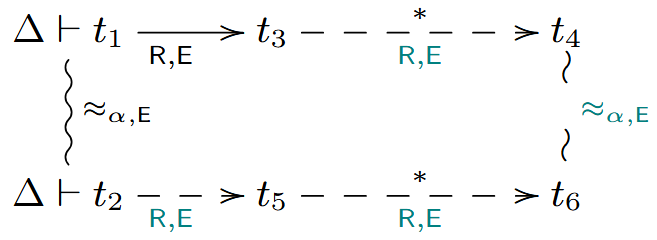
\includegraphics[scale=.5]{E-coherence.png}}
\end{center}
%\end{mdframed}
%\caption{
%\end{figure}

\vspace{2mm}
The diagram above illustrates nominal  \theory{E}-coherence: the dashed lines represent existentially quantified reductions.

\begin{definition}
An equational theory $\theory{E}$ is called {\em a first-order equational theory} iff $\theory{E}$ is defined via a set of first-order axioms, i.e., identities of the form $\emptyset\vdash l=r$, where $l,r$ are first-order terms. First-order terms do not contain atoms, abstractions and suspended permutations on variables. 
\end{definition}

% \daniele{Add the nominal version of this proposition.} \dani{It appears in~\ref{prop:nom-e-coherence} after the definition of nominal \theory{E}-coherence. Should we not comment this proposition in first order? Or just add the proof in~\ref{prop:nom-e-coherence} ?}

%return \alert{We need this nominal version of the Proposition in first order given by Jouannaud~\cite{Jouannaud83:ConfluentandCoherent} to prove the lifting theorem for commutativity.}

\begin{theorem}\label{prop:nom-e-coherence}
Let \theory{E}
be a first-order theory, 
% and 
\theory{R} be a nominal rewrite system that is
% \theory{E}-confluent and
\theory{E}-terminating
and \theory{R,E} be \theory{E}-confluent. 
Then the \theory{R,E}- and \theory{R/E}-normal forms of any term $t$ are \theory{E}-equal iff $\to_{\theory{R,E}}$ is \theory{E}-coherent.
\end{theorem}
% \begin{proof}
%     The proof is in the Appendix (see~\ref{conj:nom-e-coherence}).
% \end{proof}

% \begin{proposition}[\cite{Jouannaud83:ConfluentandCoherent}]\label{prop:e-coherence} \daniele{Move this to the appendix.}
% Assume \theory{R} is \theory{E}-confluent and \theory{E}-terminating. Then \theory{R,E}- and \theory{R/E}-normal forms of any term $t$ are \theory{E}-equal iff \theory{R,E} is \theory{E}-coherent.
% \end{proposition}

% \begin{proof}
%     \daniele{Add the nominal version of this proof.}
% \end{proof}




In first-order rewriting, it is known that  $\theory{R,E}$-reducibility is decidable if  $\theory{E}$-matching is decidable.  Following Jouannaud et al.~\cite{JouannaudKK83:Incremental},   the existence of a finite and complete $\theory{E}$-unification 
algorithm is a sufficient condition for that decidability. 
However, solving nominal $\theory{E}$-unification problems has the additional complication of dealing with $\alpha$-equality, which significantly impacts obtaining finite and complete sets of nominal $\theory{E}$-unifiers.



%We generalise the relation $\approx_\theory{C}$ to $\caleq$ and present the extended definition of nominal rewriting modulo commutativity.

% \begin{example}
% Notice that the rules in Example~\ref{ex:narr_prenex} have two copies for dealing with the commutativity of disjunction and conjunction. If we work now with the set of identities $\theory{C} = \{\;\vdash P \lor Q \approx Q \lor P, \;\vdash P \land Q \approx Q \land P\}$, we can write the NRS as
% \[
% \begin{array}{rl}
%     a \# P & \vdash \; P \land \forall[a]Q \rightarrow \forall [a](P \land Q)\\
%     % a \# P & \vdash \; (\forall[a]Q) \land P \rightarrow \forall[a](Q \land P)\\
%     a \# P & \vdash \; P \lor \forall[a] Q \rightarrow \forall[a] (P \lor Q)\\
%     % a \# P & \vdash \; (\forall[a]Q) \lor P \rightarrow \forall[a](Q \lor P)\\
%     a \# P & \vdash \; P \land \exists[a]Q \rightarrow \exists[a](P \land Q)\\
%     % a \# P & \vdash \; (\exists[a]Q) \land P \rightarrow \exists[a](Q \land P)\\
%     a \# P & \vdash \; P \lor \exists[a]Q \rightarrow \exists[a](P \lor Q)\\
%     % a \# P & \vdash \; (\exists[a]Q) \lor P \rightarrow \exists[a](Q \lor P)\\
%     & \vdash \; \lnot (\exists[a]Q) \rightarrow \forall[a] \lnot Q\\
%     & \vdash \; \lnot (\forall[a]Q) \rightarrow \exists[a] \lnot Q\\
% \end{array}
% \]

%     We will show that we have the one-step rewrite modulo $\theory{C}$: $a\#P' \vdash S'\lor (P'\lor \exists [a]Q') \to_{\theory{R,C}} S'\lor (\exists [a](Q'\lor P'))$ with the rule $a\#P \vdash P\lor \exists[a]Q \to \exists[a](P\lor Q)$.
%     Indeed,
%     \begin{itemize}
%         \item $\Delta = \{a\#P'\}$ and $\nabla = \{a\#P\}$;
%         \item $s = S'\lor (P'\lor \exists [a]Q') \equiv \context{C}[P'\lor \exists [a]Q'] \equiv \context{C}[s']$;
%     \end{itemize}
%     If we fix $\pi=\texttt{Id}$ and $\theta = [P \mapsto P', Q \mapsto Q']$ we have:
%     \begin{itemize}
%         \item $\Delta = a\#P' \vdash a\#P' = (a\#P)[P \mapsto P', Q \mapsto Q'] = \nabla\theta$;
%         \item  $s' = P'\lor \exists [a]Q' \caleq (P \lor \exists [a]Q)[P \mapsto P', Q \mapsto Q'] = l\theta = \pi\cdot (l\theta)$;
%         \item $\context{C}[\pi\cdot(r\theta)] = \context{C}[r\theta] = \context{C}[(\exists [a](P\lor Q))[P \mapsto P', Q \mapsto Q']] = \context{C}[\exists [a](P'\lor Q')] = S' \lor (\exists [a](P'\lor Q')) \caleq t$
%     \end{itemize}
%     Thus, $a\#P' \vdash S'\lor (P'\lor \exists [a]Q') \to_{\theory{R,C}} S'\lor (\exists [a](Q'\lor P'))$.
    
    
%     Observe that since $\lor$ is a commutative symbol, we could reduce the initial term to other three possible terms, because we have two occurrences of the disjunction and thus we can ``permute'' the subterms inside the rewriting modulo $\theory{C}$.
% \end{example}

\begin{remark}\label{rmk:cunif-notfin}
Nominal $\theory{C}$-unification is not finitary when one uses freshness constraints and substitutions for representing solutions~\cite{OnSolvingNomFPequations/frocos/Washington17}, but the type of problems that generate an infinite set of $\theory{C}$-unifiers are fixed-point equations $\pi\cdot X _?{\overset{\theory{C}}{\approx}}_?  X$. For example, the nominal \theory{C}-unification problem $(a \ b)\cdot X _?{\overset{\theory{C}}{\approx}}_?  X$  has solutions $[X\mapsto a\oplus b], [X\mapsto (a\oplus b)\oplus (a \oplus b)],\ldots$ (Example~ \ref{ex:c-unification}). However, these problems do not appear in nominal $\theory{C}$-matching, which is finitary~\cite{AFormalisationofNomCmatching/entcs/Ayala-RinconSFN19}. Thus, the relation $\to_{\theory{R,C}}$ is decidable. %We will come back to this issue later on.
\end{remark}

%\daniele{There is a gap that we have to fill because narrowing uses C-unification.}




\subsection{Nominal \theory{E}-narrowing}

Now we define the nominal narrowing relation modulo $\theory{E}$, extending previous works~\cite{NominalNarrowing16}.
\begin{definition}[Nominal \theory{E}-narrowing]\label{def:narr-C} 
% \daniele{(Generalise to E)}
The \emph{one-step \theory{E}-narrowing relation} $(\Delta\vdash s) \rightsquigarrow_{\theory{R,E}} (\Delta' \vdash t)$ is the least relation such that for any $(\nabla\vdash l\rightarrow r)\in \theory{R}$,  position $\context{C}$, term $s'$, permutation $\pi$, and substitution $\theta$, 
    % \vspace{-2mm}
    \begin{prooftree}
    \AxiomC{$s\equiv \context{C}[s']$}
    \AxiomC{$\Delta'\vdash \big(\nabla\theta,~\Delta\theta,~ s'\theta \ealeq \pi\cdot (l\theta), \,(\context{C}[\pi\cdot r])\theta \aleq t\big)$}
    \RightLabel{.}
    \BinaryInfC{$(\Delta\vdash s) \rightsquigarrow_{\theory{R,E}}^\theta (\Delta' \vdash t) $}
    \end{prooftree}
where $(\Delta',\theta) \in {\cal U}_{\theory{E}}( \nabla\vdash l,  \Delta\vdash  s')$.  We will write only $(\Delta\vdash s) \rightsquigarrow_{\theory{R,E}} (\Delta' \vdash t)$, omitting the $\theta$, when it is clear in the context.

The \emph{nominal \theory{E}-narrowing relation} $(\Delta \vdash s) \rightsquigarrow_{\theory{R,E}}^* (\Delta' \vdash t)$ is 
%the reflexive transitive closure of the one-step $\rightsquigarrow_{\theory{R,E}}$ relation, that is,
the least relation that includes $\rightsquigarrow_{\theory{R,E}}$ and is closed by reflexivity and transitivity of $\rightsquigarrow_{\theory{R,E}}$, i.e., it  satisfies:
\begin{enumerate}
    \item for all $\Delta, s, s'$ we have $(\Delta \vdash s) \rightsquigarrow_{\theory{R,E}}^* (\Delta \vdash s')$ if $\Delta \vdash s \aleq s'$;
    \item  for all  $\Delta, \Delta', \Delta'',s, t$ and $u$: if  $(\Delta \vdash s) \rightsquigarrow_{\theory{R,E}}^* (\Delta' \vdash t)$ and $(\Delta' \vdash t) \rightsquigarrow_{\theory{R,E}}^* (\Delta'' \vdash u)$ then $(\Delta \vdash s) \rightsquigarrow_{\theory{R,E}}^* (\Delta'' \vdash u)$.
\end{enumerate}
\end{definition}
%
The permutation $\pi$ and substitution $\theta$ in the definition above are found by solving the nominal  $\theory{E}$-unification problem $(\nabla\vdash l) \; _?{\overset{\theory{E}}{\approx}}_? \; (\Delta\vdash  s')$.

\begin{remark} Note that decidability of $\rightsquigarrow_\theory{R,E}$ relies on the existence of an algorithm for nominal \theory{E}-unification. 
%that generates a \alert{finite} minimal set of solutions. \alert{Does it need to be finite?? Not for one-step narrowing?} 
In this work, we will focus  on the theory \theory{C}, for which a nominal unification algorithm exists. %\alert{but it is not finitary!}

%From now on, our  are concentrated on  $\to_{\theory{R/C}}, \to_{\theory{R,C}}$ and $\enarrow{R,C}$.
\end{remark}



% \begin{example}Consider the rewrite rule
% $R=\{h(f((b\ c)\cdot Z,Z))\to f(h(Z),h(Z)) \}$ and suppose we want to give one narrowing step to  $h(f((a\ c)\cdot X, X))\rightsquigarrow $: (f is commutative)

% I have to solve the unification problem $h(f((a\ c)\cdot X, X))\approx^?h(f((b\ c)\cdot Z,Z))$
% \end{example}


% \daniele{Example that might give infinite branches $(f^C((a\ b) \cdot X, g(Y)),f^C(h(a), X))$ where $f^C$ satisfies commutativity $\{f^C(Y, X)=f^C(X,Y)\}$ and consider the rewrite rule $\{g(Y)\to h(Y)\}$.\\
% My unification problem after one step narrowing is : $f^C((a\ b) \cdot X, h(Y)) \caleq^? f^C(h(a), X)$}

% \daniele{Put in the appendix: the Washington's C-unification rules, definition of solution}

% \begin{example}
%     Consider the NRS with a set of rewrite rules $R=\{ \ \vdash g(Z) \to h(Z)\}$ and the set of commutativity theory $\theory{C} =\{ \ \vdash f^C(X,Y) \approx f^C(Y,X)\}$.
    
%     Let $\ \vdash f^C((a\ b)\cdot X, g(Y))$ and $\ \vdash f^C(h(a),X)$ be nominal terms that we want to unify using nominal narrowing modulo \theory{C}.
%     Observe that we can apply first one-step of narrowing, then we get a branch that yields infinite branches due to the fixed-point equation (see Figure~\ref{fig:tree}).


% $\ \vdash f^C((a\ b)\cdot X, g(X))$ and $\ \vdash f^C(h(g(Y)),X)$ 
% \end{example}

%     \begin{figure}[h!]
% \center{
% \boxed{
% \xymatrix{
%   \big{(} \emptyset, \ f^C((a\ b)\cdot X, g(Y)) \approx_? f^C(h(a),X) \big{)} \ar@{~>}^{}[d]  &  
%   % \ar@{~>}[dl] \ar@{~>}[dr]
%   & &\\
%     \big{(} \emptyset, \ f^C((a\ b)\cdot X, h(Y)) \approx_? f^C(h(a),X) \big{)}  \ar@{=>}[d] \ar@{=>}[dr] &  
%     % \ar@{=>}^{b}[d]
%     &  &\\  
%   \big{(} \emptyset, \ (a\ b)\cdot X \approx_? h(a)\ ,\ h(Y) \approx_? X \big{)} \ar@{=>}^{\theta_1=[X\mapsto h(Y)]}[d] &   \big{(} \emptyset, \ (a\ b)\cdot X \approx_? X\ ,\  h(Y) \approx_? h(a) \big{)} \ar@{=>}^{\theta_3=[Y\mapsto a]}[d]
%   % \ar@{~>}^{c}[d]
%   % \ar@{~>}[dr]\ar@{~>}[dl]
%   &  &\\
%   \big{(} \emptyset, \ (a\ b)\cdot h(Y) \approx_? h(a)\ \big{)} \ar@{=>}^{\theta_2=[Y\mapsto b]}[d] & \big{(} \emptyset, \ (a\ b)\cdot X \approx_? X\ ,\  h(a) \approx_? h(a) \big{)}  \ar@{=>}[d] \ar@{=>}[dr] &  &\\
%   \big{(} \emptyset, h(a) \approx_? h(a)\ \big{)} & \vdots &  & \vdots\\
% }
% }
% }
% \caption{ }\label{fig:narrow}
% \end{figure}

% \begin{figure}[!t]
%     \centering
%     \includegraphics[scale=.5]{branch.png}
%     \caption{Infinite tree}
%     \label{fig:tree}
% \end{figure}

%\dani{VER EXEMPLO}

Since nominal $\theory{C}$-narrowing uses nominal $\theory{C}$-unification, which is not finitary when we use pairs $(\Delta', \theta)$ of freshness contexts and substitutions to represent solutions, following Remark~\ref{rmk:cunif-notfin}, we conclude that our nominal $\theory{C}$-narrowing trees are infinitely branching. The following example illustrates these infinite branches.
\begin{example}[Cont. Example~\ref{ex:c-unification}]\label{ex:narrow}
    Consider the signature $\Sigma = \{h:1, f^\theory{C}:2, \oplus: 2\}$, where $f^\theory{C}$ and $\oplus$ are commutative symbols.
    Let $R=\{ \ \vdash h(Y) \to Y ,\ \vdash f^\theory{C}([a][b]\cdot Z, Z) \to f^\theory{C}(h(Z),h(Z)) \}$ be a set of rewrite\footnote{$\vdash l\to r$ denotes $\emptyset\vdash l\to r$.} rules. 
    Let $\ \vdash h(f^\theory{C}([b][a]X,X))$ be a nominal term that we want to apply nominal \theory{C}-narrowing to.
    Observe that we can apply one step of narrowing, and then we obtain a branch that yields infinite branches due to the fixed-point equation (see Figure~\ref{fig:enter-label5}).

    \begin{figure}[!t]
    \centering
    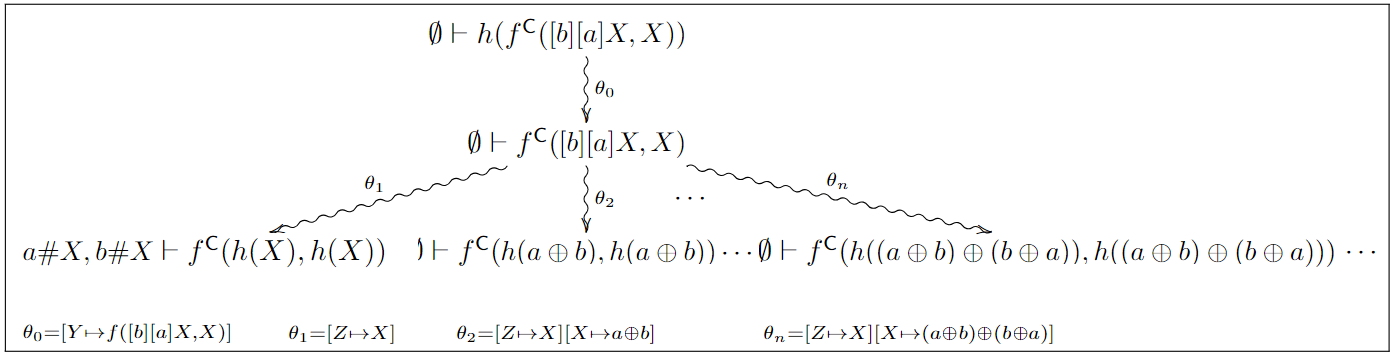
\includegraphics[scale=.59]{narrowtree6.png}
    \caption{Infinitely branching tree}
    \label{fig:enter-label5}
    \end{figure}
%     \end{example}

% \begin{example}[Cont. Example~\ref{ex:narrow}]\label{ex:contnarrow} \dani{Fix the example}
%     Here we bring all computations made in Example~\ref{ex:narrow}.

    The first narrowing step is $\emptyset \vdash h(f^\theory{C}([b][a]X,X)) \enarrow{R,C} \emptyset \vdash f^\theory{C}([b][a]X,X)$, using the rule $\ \vdash h(Y) \to Y$.
    The substitution $\theta_0= [Y\mapsto f^\theory{C}([b][a]X,X)]$ was computed in Example~\ref{ex:c-unification} when solving the \theory{C}-unification problem  $(\emptyset\vdash h(Y)) \; _?{\overset{\theory{C}}{\approx}}_? \; (\emptyset\vdash  h(f^\theory{C}([b][a]X,X))).$
    
    
    %Using the Nominal \theory{C}-unification algorithm we get the following:
% {\small
% $$
% \begin{array}{l}
%     (\emptyset, \mathtt{Id}, \{h(Y) \; _?{\overset{\theory{C}}{\approx}}_? \; h(f([b][a]X,X))\}) \quad \Longrightarrow_{(\caleq \text{\ app})} \\ 
%     \qquad \qquad  \qquad \Longrightarrow_{(\caleq \text{\ app})}  (\emptyset, \mathtt{Id}, \{Y \; _?{\overset{\theory{C}}{\approx}}_? \; f([b][a]X,X)\}) \\
%     \qquad \qquad \qquad \Longrightarrow_{(\caleq \text{\ inst})}  (\emptyset, \theta_0 = [Y\mapsto f([b][a]X,X)], \{f([b][a]X,X) \; _?{\overset{\theory{C}}{\approx}}_? \; f([b][a]X,X)\})  \\
%     \qquad \qquad \qquad \Longrightarrow_{(\caleq \text{\ refl})}  (\emptyset, \theta_0 = [Y\mapsto f([b][a]X,X)], \emptyset)\\
% \end{array}
% $$
% }
% Thus, we get the \theory{C}-solution $(\emptyset, \theta_0)$.

The other infinite narrowing steps are generated due to the fixed-point equation found in the process of solving the \theory{C}-unification problem 
$(\emptyset\vdash f^\theory{C}([a][b]Z,Z)) \; _?{\overset{\theory{C}}{\approx}}_? \; (\emptyset\vdash  f^\theory{C}([b][a]X,X))$, computed in Example~\ref{ex:c-unification}.
Composing the fixed-point solutions with $(\emptyset, \theta_1)$ that we had, we get the substitutions $\theta_1 = [Z\mapsto X]$, $\theta_2 = [Z\mapsto X][X\mapsto a \oplus b]$ and $\theta_3 = [Z\mapsto X][X\mapsto (a \oplus b)\oplus(a \oplus b)]$ of our narrowing steps in Figure~\ref{fig:enter-label5}.
 
\end{example}


%%%%%%%%%%%%%%%%%

% , and illustrate it with two examples.





% \daniele{We have to talk about the infinite branches of our narrowing tree.. } \dani{dito acima da definição 3.2.2}


% If $\Delta \vdash s \to_\theory{R,C}^* t$ and $\Delta \vdash s \to_\theory{R,C}^* t'$, then we say a nominal rewrite system $\theory{R}$ is \emph{$\theory{C}$-confluent} when there exists a term $u$ such that $\Delta \vdash t \to_\theory{R,C}^* u$ and $\Delta \vdash t' \to_\theory{R,C}^* u$.
% Also, $\theory{R}$ is said to be \emph{$\theory{C}$-terminating} if there is no infinite rewrite modulo $\theory{C}$ sequence.
% A NRS $\theory{R}$ is called \emph{$\theory{C}$-convergent} if it is $\theory{C}$-confluent and $\theory{C}$-terminating.
 
 The following proposition shows that each nominal narrowing step corresponds to a nominal rewriting step, using the same substitution $\theta$.
 %is an extension of a remark made in\cite{JouannaudKK83:Incremental} to the nominal syntax and for equational theories \theory{E}.
 % the commutative case.


\begin{proposition}\label{prop:narrow-to-rewriting}
Let \theory{E} be an equational theory for which a complete \theory{E}-unification algorithm exists. $(\Delta_0\vdash s_0) \rightsquigarrow_{\theory{R,E}}^{\theta} (\Delta_1 \vdash s_1) $ implies $\Delta_1\vdash (s_0 \theta ) \rightarrow_{\theory{R,E}}  s_1 $.
\end{proposition}

\begin{proof}
    Indeed, suppose we have $(\Delta_0\vdash s_0) \rightsquigarrow_{\theory{R,E}}^{\theta} (\Delta_1 \vdash s_1) $. The narrowing step guarantees that for a substitution $\theta$, some permutation $\pi$, and a rule $\nabla\vdash l\to r\in \theory{R}$, the following holds:  
    \begin{itemize}
        \item $s_0 \equiv \context{C}[s'_0]$ and $\Delta_1\vdash \big(\nabla\theta,~\Delta_0\theta,~ s'_0\theta \ealeq \pi\cdot (l\theta), \,(\context{C}[\pi\cdot r])\theta \aleq s_1\big)$. 
        % \daniele{This means that $\theta$ satisfies $\Delta_0$ with $\Delta_1$.}
    \end{itemize}

   From the items above, it is easy to verify  the following:
   \begin{itemize} 
   \item $s_0\theta \equiv \context{C}\theta[s'_0\theta]$; and    $\Delta_1 \vdash (\nabla\theta', s_0'\theta \ealeq \pi\cdot (l\theta'), \context{C}\theta[\pi\cdot(r\theta')] \aleq s_1)$, 
   \end{itemize} 
   and  by the definition of rewrite modulo $\theory{E}$,  it implies that  $\Delta_1 \vdash s_0\theta \rightarrow_{\theory{R,E}} s_1$.
    We need to fix the substitution $\theta$ used in the narrowing step as $\theta'$, and the result follows.
\end{proof}
% \begin{tcolorbox}

%%%%%

\section{Nominal Lifting Theorem modulo \theory{E}}\label{section:NomLiftingModuloC}

In this section, we assume $\theory{R}\cup \theory{E}$ an ENRS such that  $\theory{R}=\{\nabla_i\vdash l_i\to r_i\}$ is $\theory{E}$-convergent NRS, \theory{E} is compatible with $\vdash$ and substitutions and that there exists a complete \theory{E}-unification algorithm. We want to extend Proposition~\ref{prop:narrow-to-rewriting}  and establish correspondence between finite sequences of nominal $\theory{E}$-narrowing steps and sequences of nominal $\theory{E}$-rewriting steps. This result corresponds to the classical Lifting Theorem (\cite{Hullot80,JouannaudKK83:Incremental,NominalNarrowing16}) which will be extended to the nominal relations $\rightsquigarrow_{\theory{R,E}}$ and $\to_{\theory{R,E}}$. The Lifting Theorem relates narrowing steps to rewriting steps. It is fundamental to guarantee that one can use the narrowing relation to solve \theory{T}-unification problems when \theory{T} is a convergent equational theory. The extension to the \theory{R\cup E}-Lifting Theorem would allow us to solve nominal unification problems modulo $\theory{R}\cup \theory{E}$.

We start by defining a normalised substitution with respect to the relation $\to_{\theory{R,E}}$:
%

% \alert{Check this $R,E$-normal form and in the proof of Lemma 4.4}
\begin{definition}[Normalised substitution w.r.t $\to_{\theory{R},\theory{E}}$]
A substitution $\theta$ is \emph{normalised in $\Delta$ with relation to $\to_{\theory{R,E}}$} if $\Delta \vdash X\theta$ is a $\theory{R,E}$-normal form  for every $X$. A substitution $\theta$ {\em satisfies the freshness context} $\Delta$ iff there exists a freshness context $\nabla$ such that $\nabla \vdash a\#X\theta$ for each $a\#X \in \Delta$. In this case, we say that $\theta$ satisfies $\Delta$ with $\nabla$. The minimal such $\nabla$ is $\nfpair{\Delta\theta}$.
\end{definition}


% \daniele{TODO: Write an example of a narrowing step with one of the rewrite rules in Example 3.1 and check what happens with the context of the corresponding rewriting step. Use a reduction $\Delta\vdash s \rightsquigarrow t$ with some $\Delta$ that is different from the contexts in the rules. I want to understand this $\Delta_1/\Delta_0$ doubt. } \dani{done}

The following example illustrates the technique used in the proof of Lemma~\ref{lem:correctness}.
\begin{example}\label{ex:correct-example}
    Consider the rules $R_3: a\# P \vdash P\land\exists[a]Q\to \exists[a](P\land Q)$ and $R_6: \emptyset \vdash \neg(\forall[a]Q)\to \exists[a]\neg Q$.

    Let $(\Delta_0\vdash s_0) \rightsquigarrow^{\theta_0}_{R_6} (\Delta_1\vdash s_1) \rightsquigarrow^{\theta_1}_{R_3} (\Delta_2\vdash s_2)$ be a narrowing derivation, illustrated in Figure~\ref{fig:illustrate-example} such that:
    \begin{itemize}
        \item $\Delta_0 \equiv \emptyset$ and $s_0 \equiv P_1\land\neg(\forall[b]Q_1)$
        \item $\Delta_1 \equiv \{a\#Q_1\}$ and $s_1 \equiv P_1\land \exists[a](\neg (a\ b)\cdot Q_1)$ 
        % \daniele{your abstraction is in $[b]$ because you isolated $Q_1$ instead of $Q$ in your unification step.}
        \item $\Delta_2 \equiv \{a\# Q_1, a\#P_1\}$ and $s_2 \equiv \exists[a](P_1\land\neg(a\ b)\cdot Q_1)$ 
        % \daniele{I don't understand why you have two existential. The initial term only had one $\exists$. And the rule does not add existential. Also, you are missing a constraint in $\Delta_2$.}
    \end{itemize}
    Let $\rho$ be a substitution that satisfies $\Delta_2$ with $\Delta$. Then, there exists a rewriting derivation
    $$\Delta\vdash s_0\rho_0 \to_\theory{R,C} s_1\rho_1 \to_\theory{R,C} s_2\rho$$
    where $\Delta\vdash \Delta_0\rho_0$, $\Delta\vdash \Delta_1\rho_1$ and $\rho_0=\theta_0\theta_1\rho$, $\rho_1 = \theta_1\rho$.

    \begin{figure}[!t]
    \begin{mdframed}
    \begin{center}
        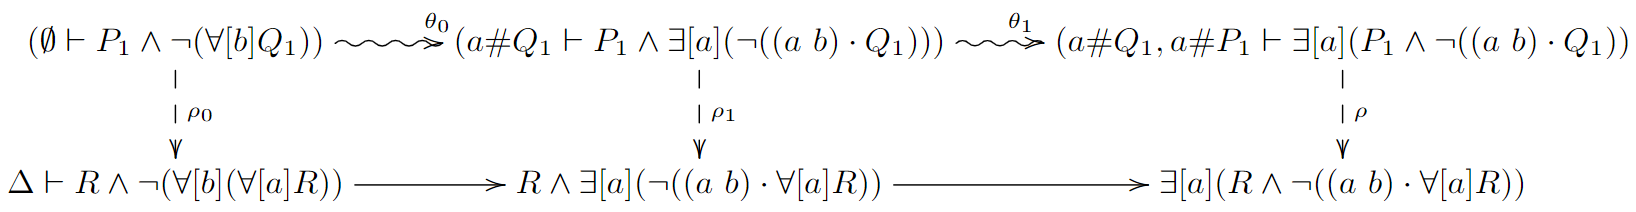
\includegraphics[scale=.52]{ex-narrow-to-rew2.png}
    \end{center}
    \end{mdframed}
    % \alert{Either you have to use $\rho$ instead of $\rho_2$ or write $\rho_2=\rho$ somewhere.}
    \caption{Illustration of Example~\ref{ex:correct-example}}\label{fig:illustrate-example}
    \end{figure}
    Supposing that $\rho = [Q_1\mapsto \forall[a]R,P_1\mapsto R]$, and $\Delta =\{a\# R\}$, we have
    \begin{itemize}
        \item $\Delta\vdash \Delta_2\rho = \{a\#Q_1,a\#P_1\}\rho = \{a\#\forall[a]R,a\#R\} = \{a\#R\}$
        \item $\theta_0 = [Q \mapsto (a\ b)\cdot Q_1]$
         and  $\theta_1 = [P'\mapsto P_1, Q'\mapsto \neg((a\ b)\cdot Q_1)]$ 

        \item $\rho_1 = \theta_1\rho = [P' \mapsto R, Q'\mapsto \neg((a\ b)\cdot \forall[a]R), Q_1\mapsto \forall[a]R, P_1\mapsto R]$
        \item $\rho_0 = \theta_0\rho_1 = [Q\mapsto(a\ b)\cdot \forall[a]R, P' \mapsto R, Q'\mapsto \neg((a\ b)\cdot \forall[a]R), Q_1\mapsto \forall[a]R, P_1\mapsto R]$
        \item $\Delta\vdash \Delta_1\rho_1 = (a\#Q_1)\rho_1 = a\# \forall[a]R = \emptyset$ and  $\Delta\vdash \Delta_0\rho_0 = \emptyset$
    \end{itemize}
\end{example}

% \alert{POLISH: The next result shows that the correspondence between narrowing and rewriting is preserved by application of substitution.}

The next result shows that the rewriting step generated by the narrowing step
is preserved by application of substitution if the theory \theory{E} is compatible (Definition~\ref{def:e-compatible}), that is, $\vdash$ is closed by substitutions.
\begin{lemma}{($\rightsquigarrow_{\theory{R,E}}$ to $\to_{\theory{R,E}}$)}
\label{lem:correctness}
Let \theory{E} be compatible with $\vdash$ by substitutions and  $(\Delta_0 \vdash s_0) \rightsquigarrow_{\theory{R,E}}^\theta (\Delta_1 \vdash s_1) $. Then, for any substitution $\rho$ that satisfies $\Delta_1$ with $\Delta$,
%, i.e., there exists $\Delta$ such that $\Delta \vdash \Delta_0\rho$,
the following holds
$$\Delta \vdash (s_0 \theta )\rho \rightarrow_{\theory{R,E}}  s_1 \rho$$
%where $\theta$ is the substitution applied in the narrowing step.
In particular, $\Delta$ will be $\nfpair{\Delta_1\rho}$.
\end{lemma}
\begin{proof}
From Proposition~\ref{prop:narrow-to-rewriting}:
$(\Delta_0\vdash s_0) \rightsquigarrow_{\theory{R,E}}^{\theta} (\Delta_1 \vdash s_1) $ implies $\Delta_1\vdash (s_0 \theta ) \rightarrow_{\theory{R,E}}  s_1 $.
By \theory{E}-compatiblity of derivability with substitutions $\Delta_1 \vdash s_0\theta \rightarrow_{\theory{R,E}} s_1$ gives: 

\begin{itemize}
    \item $(s_0\theta)\rho \equiv (\context{C}\theta[s'_0\theta])\rho = \context{C}\theta\rho[(s'_0\theta)\rho]$
    \item $\Delta_1 \vdash \nabla\theta$ implies  $\nfpair{\Delta_1\rho} \vdash \nabla\theta\rho$
    \item $\Delta_1 \vdash s_0'\theta \ealeq \pi\cdot (l\theta)$ implies $\nfpair{\Delta_1\rho} \vdash s_0'\theta\rho \ealeq (\pi\cdot(l\theta))\rho = \pi\cdot(l\theta\rho)$
    \item $\Delta_1 \vdash \context{C}\theta[\pi\cdot(r\theta)] \aleq s_1$ implies $\nfpair{\Delta_1\rho} \vdash \context{C}\theta\rho[\pi\cdot(r\theta\rho)] = (\context{C}\theta[\pi\cdot(r\theta)])\rho \aleq s_1\rho$
\end{itemize}
which implies that $\nfpair{\Delta_1\rho} \vdash (s_0\theta)\rho \rightarrow_{\theory{R,E}} s_1\rho$.
Note that we need $\rho$ satisfying $\Delta_1$ with $\Delta$ to guarantee that when we instantiate $\Delta_1$ we do not have any inconsistency with the freshness constraints in $\Delta_1$.
\end{proof}

The following result (correctness) states that a finite sequence of rewriting steps exists for each finite sequence of narrowing steps.

%We begin by presenting that a correctness result is preserved for finite sequences of narrowing steps as follows.

\begin{lemma}{($\rightsquigarrow_{\theory{R,E}}^*$ to $\to_{\theory{R,E}}^*$)}\label{theo:narrowtorewrite}
Let \theory{E} be compatible with $\vdash$ by substitutions and  $(\Delta_0\vdash s_0) \rightsquigarrow^*_{\theory{R,E}} (\Delta_n \vdash s_n) $ be a nominal \theory{E}-narrowing derivation. 
Let $\rho$ be a substitution satisfying $\Delta_n$ with  $\Delta$.
$$(\Delta_0\vdash s_0) \rightsquigarrow^{\theta_0}_{\theory{R,E}} (\Delta_1 \vdash s_1) \rightsquigarrow^{\theta_1}_{\theory{R,E}}  \ldots \rightsquigarrow^{\theta_{n-1}}_{\theory{R,E}} (\Delta_n \vdash s_n) $$
%such that $\Delta \vdash \Delta_0\rho$. 
Then, there exists a nominal \theory{E}-rewriting derivation 
% \vspace{-2mm}
$$\Delta\vdash s_0\rho_0  \rightarrow_{\theory{R,E}} \ldots \rightarrow_{\theory{R,E}} s_i\rho_i \rightarrow_{\theory{R,E}}\ldots   \rightarrow_{\theory{R,E}} s_{n-1}\rho_{n-1}\rightarrow_{\theory{R,E}} s_n\rho$$ 
such that $\Delta\vdash \Delta_i\rho_{i}$ and $\rho_{i}=\theta_{i}\ldots \theta_{n-1}\rho$, for all $0\leq i < n$. In other words,
% \vspace{-1mm}
$\Delta\vdash (s_0 \theta )\rho \rightarrow^*_{\theory{R,E}}  s_n \rho $
where $\theta=\theta_0\theta_1\ldots \theta_{n-1}$.
\end{lemma}
% \begin{proof}
%     The proof is in Appendix~\ref{app:proofs} and illustrated by Figure~\ref{fig:narrrew}.
% \end{proof}
\begin{proof}
By induction on the length $n\geq 1$ of the narrowing derivation $(\Delta_0\vdash s_0) \rightsquigarrow^{n}_{\theory{R,E}} (\Delta_n \vdash s_n)$, 
using the one-step result proved in Lemma~\ref{lem:correctness}. (We start the induction for $n=1$ because the case for $n=0$ holds trivially and gives no additional insight.) 
\begin{itemize}
    \item \textbf{Base Case:} For $n=1$, 
    % we have by assumption that $\rho_0 = \theta_0\rho$ and $\Delta \vdash \Delta_0\rho_0$. From Lemma~\ref{lem:correctness}, there is a step 
    % $\Delta \vdash s_0\rho_0 = (s_0\theta_0)\rho \rightarrow_{\theory{R,C}} s_1\rho$, and the result follows.
    we have $(\Delta_0\vdash s_0) \rightsquigarrow_{\theory{R,E}} (\Delta_1 \vdash s_1)$ and by Lemma~\ref{lem:correctness}, for any $\rho$ satisfying $\Delta_1$ with $\Delta$ we have $\Delta \vdash  (s_0\theta_0)\rho \rightarrow_{\theory{R,E}} s_1\rho$. Since $\Delta\vdash \Delta_1\rho$, and by the narrowing step $\Delta_1\vdash \Delta_0\theta_0$, we get $\Delta\vdash \Delta_0\theta_0\rho$. Taking $\rho_0 = \theta_0\rho$, we have the result
    $\Delta\vdash s_0\rho_0 \to_\theory{R,E} s_1\rho$
    such that $\Delta\vdash \Delta_0\rho_0$.
    \item \textbf{Induction Step:} Assume that the result holds for $n>1$. Then 
    $(\Delta_0 \vdash s_0) \rightsquigarrow^{n}_{\theory{R,E}} (\Delta_n \vdash s_n)$
    implies that there exists a rewriting derivation
    $\Delta \vdash s_0\rho_0 \rightarrow^{n}_{\theory{R,E}} s_n\rho$, for some $\rho$ satisfying $\Delta_n$ with $\Delta$
    % \daniele{By unfolding the definition of $\rho_i$, the rewriting derivation is as  $\Delta \vdash s_0\rho_0 \equiv (s_0\theta_0)\rho\rightarrow^{i+1}_{\theory{R,C}} s_i \theta_i\ldots \theta_{n-1}\rho\equiv s_i\rho_i$,}
    and Figure~\ref{fig:narrrew} illustrates this setting.
    
    We want to show that the result follows for $n+1$. Consider the narrowing step 
    $$(\Delta_n \vdash s_n) \rightsquigarrow^{\theta_n}_\theory{R,E} (\Delta_{n+1} \vdash s_{n+1}).$$
    
    
   By Lemma~\ref{lem:correctness}, for any substitution, let's name it $\sigma$, that satisfies $\Delta_{n+1}$ with $\Delta$ {\bf (H1)}
    % there exists $\Delta$ that satisfies $\Delta_i\rho_{i+1}$, and we have 
    we have
    \begin{equation}\label{eq:narrow}
        \Delta \vdash (s_n\theta_n)\sigma \to_{\theory{R,E}} s_{n+1}\sigma
    \end{equation}
  
    %$\Delta \vdash s_0\rho_0 \rightarrow^{n+1}_{\theory{R,E}} s_{n+1}\sigma$, for some $\sigma$ that satisfies $\Delta_{n+1}$ with $\Delta$. That is, $$\Delta \vdash s_0\rho_0 \to^n_\theory{R,E} s_n\rho \to_{\theory{R,E}} s_{n+1}\sigma.$$
    
    
    Take $\rho = \theta_n\sigma$. Note that  $\rho$ satisfies $\Delta_n$ with $\Delta$:
    \begin{enumerate}[\bf (H1)]
        \item $\Delta\vdash \Delta_{n+1}\sigma$.
        \item By Definition~\ref{def:narr-C}: $\Delta_{n+1}\vdash \Delta_n\theta_n$.
        \item From {\bf (H2)} and \theory{E}-compatibility Definition~\ref{def:e-compatible}(1) generalised to \theory{E}:  $\langle\Delta_{n+1}\sigma\rangle_{nf} \vdash \Delta_n\rho$.
    \end{enumerate}
     Thus, from {\bf (H1)} and {\bf (H3)} it follows that  $\Delta\vdash \Delta_n\rho$.
    By the induction hypothesis,  we have 
    $$\Delta \vdash s_0\theta_0\ldots\theta_{n-1}\rho \rightarrow^{n}_{\theory{R,E}} s_n\rho$$
    with $\Delta\vdash \Delta_i\rho_i$ 
    and $\rho_i = \theta_i\ldots\theta_{n-1}\rho$, for every $i=1,\ldots, n$. Hence,
    $$\Delta \vdash s_0\theta_0\ldots\theta_{n-1}\theta_n\sigma \to^{n}_{\theory{R,E}} s_n\theta_n\sigma \overset{\eqref{eq:narrow}}{\to}_{\theory{R,E}} s_{n+1}\sigma,$$
    and the result follows.
%
    % Note that $\Delta\vdash \Delta_{n+1}\sigma$ and by the narrowing step $\Delta_{n+1}\vdash \Delta_n\theta_n$ thus $\Delta\vdash \Delta_n\theta_n\sigma = \Delta_n\rho$.
\end{itemize}
%
%Notice that $\rho_i$ is $\theory{R,E}$-normalised if $\rho_0$ is $\theory{R,E}$-normalised.
\end{proof}


% With Theorem~\ref{theo:narrowtorewrite} we have extended the converse part of the Nominal Lifting Theorem
% %(Theorem~\ref{theorem:lifting}), from the previous chapter,
% to the nominal rewriting/narrowing modulo $\theory{C}$.

% \begin{figure}
% \small
% $$
% \boxed{
% \textnormal{
%  \xymatrix{
% (\Delta_0 \vdash s_0) \ar@{~>}[r]^{\theta_0} & (\Delta_1 \vdash s_1) \ar@{~>}[r]^{*} & (\Delta_i \vdash s_i) \ar@{~>}[r]^{\theta_i} & (\Delta_{i+1} \vdash s_{i+1}) \ar@{~>}[r]^{*} & \ldots \ar@{~>}[r]^{\theta_n} &(\Delta_n \vdash s_n)\\
% \Delta  \vdash s_0\rho_0 \ar@{<--}[u]_{\rho_{0}}\ar[r] & s_1\rho_1\ar@{<--}[u]_{\rho_1}\ar[r]^{*} & s_i\rho_i\ar[r]\ar@{<--}[u]_{\rho_i} &  s_{i+1}\rho_{i+1}\ar@{<--}[u]_{\rho_{i+1}} \ar[r]^{*} & \ldots \ar[r] & s_n\rho_n \ar@{<--}[u]_{\rho_{n}}
% } 
% }
% }
% $$
% \caption{Corresponding Narrowing to Rewriting Derivations\label{fig:narrrew}}
%  \end{figure}

\begin{figure}[!t]
    \centering
    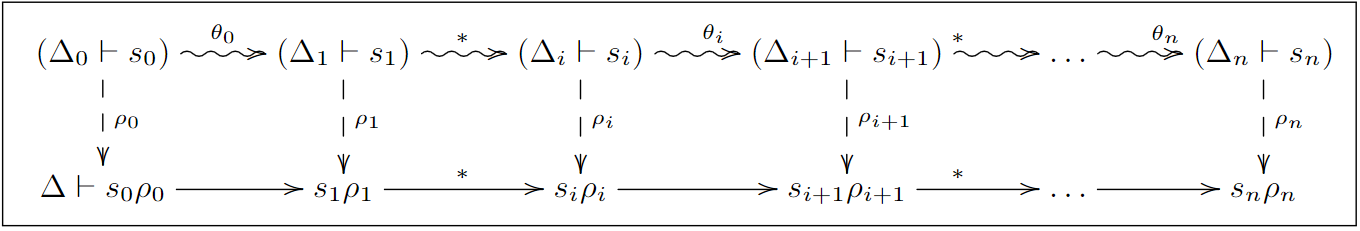
\includegraphics[scale=.55]{narrow-to-rewrite.png}
    \caption{Corresponding Narrowing to Rewriting Derivations}
    \label{fig:narrrew}
\end{figure}

% \daniele{Add some text explaining the next result.}
The proof of the converse (completeness) is more challenging. Nevertheless, for one-step rewriting to one-step narrowing, the result holds with no further problems:


% \alert{Check this $R,E$-normal form and in the proof of this Lemma. Is it $R,E$ or $R/E$-nf? }\dani{we want to use a R,E-normalised subst because we are using R,E-steps. However, in the 4.5 we have coherence, so R,E- and R/E-nf are E-equal}
\begin{lemma}{($\to_{\theory{R,E}}$ to $\rightsquigarrow_{\theory{R,E}}$)}\label{alem:rewrite-narr}
 Let $\Delta_0\vdash s_0$ be a nominal term in context and $V_0$ a finite set of variables containing $V=V(\Delta_0,s_0)$.
Let   $\rho_0$ be a $\theory{R,E}$-normalised substitution, with $\dom{\rho_0}\subseteq V$, that satisfies $\Delta_0$ with  $\Delta$ and
$$\Delta \vdash s_0\rho_0=t_0 \to_{\theory{R,E}} t_1.$$
Then, there exists a nominal  \theory{R,E}-narrowing step
$$(\Delta_0 \vdash s_0) \rightsquigarrow^\theta_{\theory{R,E}} (\Delta_1 \vdash s_1),$$
for a substitution $\theta$, a finite set of variables $V_1 \supseteq V(s_0)$, and a $\theory{R,E}$-normalised substitution $\rho_1$ with $\Delta$ such that

\[(i)~\Delta \vdash s_1\rho_1 \ealeq t_1 \qquad  (ii)~\texttt{dom}(\rho_1) \subseteq V_1 \qquad (iii)~\Delta\vdash \rho_0|_V\ealeq \theta \rho_1|_V \]
\end{lemma}
\begin{proof}
Suppose that the one-step rewriting is done in a position $\context{C}_0$ of $t_0$, with substitution $\sigma$ and  rule $R_0 = \nabla_0 \vdash l_0 \to r_0 \in \theory{R}$:
%$\Delta \vdash t_0 \to_{[\context{C}_0, R_0],\theory{E}} t_1$. Then, 
\begin{mathpar}
    \inferrule*[left=(*)]{t_0\equiv \context{C}_0[t_0'] \\ \Delta \vdash \nabla_0\sigma,\; t_0' \ealeq \pi\cdot(l_0\sigma)  ,\; \context{C}_0[\pi\cdot(r_0\sigma)] \aleq t_1}{\Delta \vdash t_0 \to_{[\context{C}_0, R_0],\theory{E}} t_1}
\end{mathpar}
%That means that for some position $\context{C}_0[\_]$ we have $t_0\equiv \context{C}_0[t_0']$ and $\Delta \vdash \nabla_0\theta,\; \pi\cdot(l_0\theta) \ealeq t_0',\; \context{C}_0[\pi\cdot(r_0\theta)] \ealeq t_1$~(*).
%

The following hold:
%\dani{Check this proof and cite the compatibility of substitutions}
\begin{enumerate}[{\bf (H1)}]
    \item The variables of $R_0$ are renamed with respect to $t_0 = s_0\rho_0$ and $\Delta$ (to avoid conflicts). Thus,  $V(R_0)\cap V(\Delta, t_0) = \emptyset$ and $\texttt{dom}(\sigma) \cap V_0 = \emptyset$.  
    \item By hypothesis, $\Delta\vdash \Delta_0\rho_0$ 
    \item Since $\rho_0$ is  normalised in $\Delta$ and $\Delta\vdash s_0\rho_0\to_\theory{R,E} t_1$,  there must exist a non-variable position $\context{C}_0'$ and a subterm $s_0'$ of $s_0$ such that $s_0\equiv \context{C}_0'[s_0']$ and $\Delta \vdash s_0'\rho_0 \ealeq t_0' \ealeq \pi\cdot(l_0\sigma)$.
    %\daniele{use a $\sigma$}
\end{enumerate}
%since $V(R_0)\cap V(\Delta, t_0) = \emptyset$, because $R_0$ is a variable renamed rule with respect to $t_0 = s_0\rho_0$.

%It follows from the fact that $\rho_0$ is normalised in $\Delta$, that $\Delta \vdash s_0\rho_0 \ealeq t_0$ and $\Delta \vdash \Delta_0\rho_0$ that there exists a non-variable position $\context{C}_0'$ such that  

Define {\bf (H4)} $\theta=\rho_0\sigma$. 
%$\eta = \rho_0\cup\theta$~(**). 
Then, we have the following:
\begin{enumerate}[{\bf (H1)}]
\setcounter{enumi}{4}
    \item $\Delta \vdash \Delta_0\theta$: from {\bf (H2)} it follows that $\Delta \vdash \Delta_0\rho_0$ and $\sigma$ does not affect $\Delta_0$ since $\texttt{dom}(\sigma) = V(R_0)$.
    %\item $\Delta \vdash s_0'\eta \ealeq \pi\cdot (l_0\eta)$.
    \item Note that $s_0'\theta=s_0'\rho_0\sigma=s_0'\rho_0$ from {\bf (H1)}. Therefore, $\Delta \vdash s_0'\theta \ealeq \pi\cdot (l_0\theta)$ and $\Delta \vdash\nabla_0\theta$,
    %$\Delta \vdash s_0'\eta \ealeq \pi\cdot (l_0\eta)$ 
    and  $(\Delta,\theta)$
    %$(\Delta, \eta)$
    is a solution for the nominal \theory{E}-unification problem $(\Delta_0 \vdash s_0') \; _?\overset{\theory{E}}{{\approx}}_? \; (\nabla_0 \vdash \pi\cdot l_0)$. That is, $(\Delta, \theta)\in \mathcal{U}_\theory{E}(\Delta_0 \vdash s_0', \nabla_0 \vdash \pi\cdot l_0)$.
\end{enumerate}

% Take one solution  Then, the following hold:
% \begin{itemize} 
% \item $\Delta_1 \vdash \Delta_0\theta, \nabla_0\theta$
% \item $\Delta_1\vdash s_0'\theta \ealeq \pi\cdot(l_0\theta)$. 
% \end{itemize} 
Define $s_1$ as $s_1=\context{C}_0'[\pi\cdot r_0]\theta$ and $\Delta_1=\Delta$. Conditions {\bf (H4)} to {\bf (H6)} imply the existence of the  following nominal  \theory{E}-narrowing step:
 $$(\Delta_0 \vdash s_0) \rightsquigarrow^\theta_{\theory{R,E}} (\Delta_1 \vdash s_1).$$

Also $\Delta\vdash s_1=\context{C}_0'[\pi\cdot r_0]\theta=(\context{C}_0'[\pi\cdot r_0])\rho_0\sigma \aleq (\context{C}_0'\rho_0)[\pi\cdot r_0]\rho_0 \overset{(*)}{\approx}_{\alpha}  t_1$. Take $\rho_1={\tt Id}$ as the identity substitution, and items (i) and (ii) follow with $\dom{\rho_1}=\emptyset$ and $V_1=V(s_0)$.
Finally, it is trivial to check (iii):   $\Delta\vdash X\rho_0\ealeq  X\theta\rho_1\equiv X\rho_0\sigma{\tt Id}$, for all $X\in V$, and the result follows.



% Since $(\Delta_1, \theta)\in \mathcal{U}_\theory{E}(\Delta_0 \vdash s_0', \nabla_0 \vdash \pi\cdot l_0)$ is one least unifier of $(\Delta_0 \vdash s_0') \; _?{\approx}_? \; (\nabla_0 \vdash \pi\cdot l_0)$, in other words $(\Delta_1, \theta) \leq (\Delta, \eta)$, thus there exists a substitution $\rho'$ such that for all $X$, $\Delta \vdash X\theta\rho' \ealeq X\eta$ and $\Delta \vdash \Delta_1\rho'$.

% It remains to show the side conditions:
% \begin{itemize}
%     \item $\Delta \vdash s_1\rho_1 \ealeq t_1$: On the one hand we have $\Delta \vdash s_1\rho_1 \ealeq (\context{C}_0'[\pi\cdot r_0]\theta)\rho_1 \ealeq (\context{C}_0'[\pi\cdot r_0]\theta)\rho' \ealeq \context{C}_0'\theta\rho'[\pi\cdot r_0\theta\rho'] \ealeq \context{C}_0'\eta[\pi\cdot r_0\eta]$. Since~(**), we have $\context{C}_0'\eta[\pi\cdot r_0\eta] \ealeq \context{C}_0'\rho_0[\pi\cdot r_0\rho_0] \ealeq \context{C}_0[\pi\cdot r_0\rho_0]$. On the other hand, $\Delta \vdash t_1 \stackrel{(*)}{\ealeq} \context{C}_0[\pi\cdot r_0\theta] \ealeq \context{C}_0[\pi\cdot r_0\eta] \ealeq \context{C}_0[\pi\cdot r_0\rho_0]$.
%     \item $\texttt{dom}(\rho_1) \subseteq V_1$: Let $V_1 = (V_0\cup \texttt{Im}(\rho_0)) - \texttt{dom}(\rho_0)$ and let $\rho_1$ be such that $\Delta \vdash \rho_1 \ealeq \rho'|_{V_1}$,  with this $\alpha,\theory{E}$-equivalence, the result follows. 
%     %\dani{pq podemos tomar esses $V_1$ e $\rho_1$?}
%     \item $\Delta \vdash \rho_0|_V \ealeq \theta\rho_1|_V$: We already have that $\Delta \vdash \rho_0 \ealeq (\theta\rho_1)|_{V_0}$. We just need to apply the restriction to $V$ on both sides and the result follows.
% \end{itemize}
\end{proof}


%return \dani{This sentence needs to be removed} The challenge is that, in the first-order case, the approach to prove that each finite sequence of $\to_{\theory{R,E}}$ steps corresponds to a finite sequence of $\rightsquigarrow_{\theory{R,E}}$ steps relied on an additional property: \theory{E}-coherence. This property can be extended to the nominal framework as follows:


% \begin{tcolorbox}
%\begin{remark}\label{rmk:e-completeness}
% Nevertheless, the generalisation of one-step nominal rewrite
% % the previous lemma 
% to finite sequences of nominal rewrite steps is more problematic. 
% It relies on a property called \theory{E}-coherence, which we define in the nominal framework as follows:


%, see Figure~\ref{fig:prop3JOU} at Appendix.
% below.
%\end{remark}
% More details about the relations between $\to_{\theory{R}/\theory{E}}$ and $\to_{\theory{R},\theory{E}}$ and the property of \(\theory{E}\)-coherence can be found in Appendix~\ref{appendixFirstOrder}.
% \end{tcolorbox}

\smallskip
\smallskip


% Jouannaud et al.~\cite{JouannaudKK83:Incremental} proved, in the first-order case,  that  $\to_{\theory{R}/\theory{E}}$ and $\to_{\theory{R},\theory{E}}$ coincide, if $\to_{\theory{R},\theory{E}}$ is \theory{E}-coherent (see Figure~\ref{fig:prop3JOU}). We conjecture that the same result holds for the nominal framework, as long as \theory{E}
% is a first-order theory (it does not contain bindings and/or freshness constraints).
%It was proven, for a general theory \(\theory{E}\), in the first-order case, by , following an inductive proof, and with the  conditions  $\theory{E}$-coherence for $\to_{\theory{R},\theory{E}}$ and $\theory{E}$-confluence, to guarantee that the relations

% \begin{figure}[!t]
%     \centering
%     \begin{mdframed}
%     \centering
%     \includegraphics[scale=.5]{JKKprop3.png}
%     \end{mdframed}
% %    \alert{Decide if we are going to keep this diagram or not.  MAR: It would be nice to include it!}
%     \caption{Proposition by Jouannaud~\cite{JouannaudKK83:Incremental} used in Lemma~\ref{theo:rewritenarr}}
%     \label{fig:prop3JOU}
% \end{figure}

% \begin{conjecture}\label{prop:nom-e-coherence}
% Let \theory{E}
% be a first-order theory and  \theory{R} be a nominal rewrite system that is \theory{E}-confluent and \theory{E}-terminating. Then the \theory{R,E}- and \theory{R/E}-normal forms of any term $t$ are \theory{E}-equal iff $\to_{\theory{R,E}}$ is \theory{E}-coherent.
% \end{conjecture}
% \begin{proof}
%     The proof is future work.
% \end{proof}
% Conjecture~\ref{prop:nom-e-coherence} is used in the proof of Theorem~\ref{theo:rewritenarr}, which we call a {\em naive completeness}:
% % version of Proposition 3 in Remark~\ref{rmk:e-completeness}
% % and a draft of the proof:
% the exact conditions on the freshness contexts have to be further investigated and Conjecture~\ref{prop:nom-e-coherence} has to be proven.

% \alert{ Check the statement and fix accordingly, and check the proof.}
\begin{lemma}{($\to^*_{\theory{R,E}}$ to $\rightsquigarrow^*_{\theory{R,E}}$)}\label{theo:rewritenarr}
Let $\theory{R}{\cup}\theory{E}$ be an ENRS such that $\theory{R}$ is 
% $\theory{E}$-convergent 
\theory{E}-terminating, \theory{R,E} is \theory{E}-confluent
and $\to_{\theory{R,E}}$ is $\theory{E}$-coherent. Let $V_0$ be a finite set of variables containing $V=V(\Delta_0,s_0)$. Then, for any $\theory{R,E}$-derivation 
%---
$$\Delta \vdash t_0 = s_0\rho_0\rightarrow_{\theory{R,E}} t_1\rightarrow_{\theory{R,E}}\ldots \rightarrow_{\theory{R,E}} t_n=t_0{\downarrow}$$
%-----
to any of its $\theory{R,E}$-normal forms, say $t_0{\downarrow}$, where $\texttt{dom}(\rho_0) \subseteq V(s_0) \subseteq V_0$ and $\rho_0$ is a $\theory{R,E}$-normalised substitution that satisfies $\Delta_0$ with $\Delta$, there exist a $\theory{R,E}$-narrowing derivation 
%------
$$(\Delta_0\vdash s_0) \rightsquigarrow^{\theta_0}_{\theory{R,E}} (\Delta_1 \vdash s_1) \rightsquigarrow^{\theta_1}_{\theory{R,E}}  \ldots \rightsquigarrow^{\theta_{n-1}}_{\theory{R,E}} (\Delta_n \vdash s_n) $$
%---
%$$(\Delta_0 \vdash s_0) \rightsquigarrow_{\theory{R,E}}^* (\Delta_n \vdash s_n),$$for each $i$, $0\leq i < n$,   substitutions $\rho$ and  $\rho_i$ normalised in $\Delta$ w.r.t $\to_\theory{R,E}$  such that 
\begin{center}
(1) $\Delta\vdash \Delta_i\rho_i$; \qquad 
(2)  $\Delta \vdash s_i\rho_i \ealeq t_i$;\qquad 
(3)  $\Delta \vdash \rho_0|_V \ealeq \theta\rho_n|_V$.
\end{center}
where  $\rho_{i}=\theta_i\ldots \theta_{n-1}\rho$ and  $\theta=\theta_0\theta_1\ldots \theta_{n-1}$.
\end{lemma}
% \begin{proof}
%     The draft of the proof is in Appendix~\ref{app:proofs}.
% \end{proof}

\begin{proof}
 By induction on the number of steps $n$ applied in the derivation $\Delta \vdash t_0 = s_0\rho_0\rightarrow_{\theory{R,E}}^* t_0{\downarrow}$.

\begin{itemize}
    \item \textbf{Base Case:} For $n=1$ the result follows directly from Lemma~\ref{alem:rewrite-narr}.

    \item \textbf{Induction Step:} Let $n>1$ and assume that the result holds for sequences of  $n-1$ rewriting steps.
    Then, 
    %
    $$\Delta \vdash t_0 = s_0\rho_0\rightarrow_{\theory{R,E}} t_1\overbrace{\rightarrow_{\theory{R,E}}\ldots \rightarrow_{\theory{R,E}}}^{n-1} t_n=t_0{\downarrow}$$
    %
    Now using Lemma~\ref{alem:rewrite-narr} on the rewrite step $\Delta \vdash t_0 \to_{\theory{R,E}} t_1$.  Then, we get that 
    %
    $(\Delta_{0} \vdash s_{0}) \rightsquigarrow_{\theory{R,E}}^{\theta_{0}} (\Delta_1 \vdash s_1),$
    %
   where $\rho_0$ is a $\theory{R,E}$-normalised substitution that satisfies $\Delta_0$ with $\Delta$, and
   \begin{enumerate}[{\bf (H1)}] 
   \item  $\Delta \vdash s_1\rho_1 = t_1' \ealeq t_1$; and 
   \item $\Delta \vdash \rho_0|_V \ealeq \theta\rho_1|_V$. 
   \end{enumerate} 
   Now consider the sequence to any of the normal forms of $t_1$:
    %
      $$\Delta \vdash  t_1\overbrace{\rightarrow_{\theory{R,E}}\ldots \rightarrow_{\theory{R,E}}}^{n-1} t_n=t_1{\downarrow_\theory{R,E}}
      $$     
    %
    By the induction hypothesis, there exists  a narrowing sequence 

     %----
    $$ (\Delta_1 \vdash s_1) \rightsquigarrow^{\theta_1}_{\theory{R,E}}  \ldots \rightsquigarrow^{\theta_{n-1}}_{\theory{R,E}} (\Delta_n \vdash s_n) $$
    %%--
    with $\theta=\theta_1\ldots \theta_{n-1}$, a normalised substitution $\rho_n$ such that 
   \begin{enumerate}[{\bf (H1)}] 
   \setcounter{enumi}{2}
   \item $\Delta\vdash \Delta_i\rho_i$;
   \item  $\Delta \vdash s_i\rho_i =t_i'\ealeq t_i$, for every $i$; 
   \item $\Delta \vdash \rho_0|_V \ealeq \theta\rho_n|_V$. 
   \end{enumerate} 
   Note that from {\bf (H4)}, $\Delta\vdash s_n\rho_n=t_n'\ealeq t_n$. Since \theory{R} is \theory{E}-convergent and $\to_{\theory{R,E}}$ is \theory{E}-coherent, it follows from Theorem~\ref{prop:nom-e-coherence}, that all the normal forms  of $t_0$ are $\ealeq$-equivalent. That is, 
   $\Delta\vdash t_n'\ealeq t_1\downarrow_\theory{R,E}\ealeq t_0\downarrow_\theory{R,E}=t_n.$
    Therefore, there exists  a nominal \theory{E}-narrowing sequence
  $$(\Delta_0\vdash s_0) \rightsquigarrow^{\theta_0}_{\theory{R,E}} (\Delta_1 \vdash s_1) \rightsquigarrow^{\theta_1}_{\theory{R,E}}  \ldots \rightsquigarrow^{\theta_{n-1}}_{\theory{R,E}} (\Delta_n \vdash s_n).$$
\end{itemize}
   % The diagram that illustrates this proof is analogous to the diagram of the corresponding proof in first-order rewriting.
   % and \alert{presented in~Figure~\ref{fig:complete_diagram}.}

%    \bigskip
%     \alert{old version}
    
%     Then, we have $$\Delta \vdash t_0 = s_0\rho_0\to_{\theory{R,E}}^{\{n-1\}} t_{n-1}\rightarrow_{\theory{R,E}} t_n\equiv t_0{\downarrow},$$ 
%     %%---
%     for some $t_{n-1}$.
%     By the induction hypothesis, \alert{you cannot apply induction hypothesis here, because in the sequence to $t_{n-1}$ is not a normal form. The result only holds for reductions until the normal form} there exists a nominal $\theory{R,E}$-narrowing derivation 
%     %----
%     $$(\Delta_0 \vdash s_0) \rightsquigarrow^{\{n-1\}}_{\theory{R,E}} (\Delta_{n-1} \vdash s_{n-1}),$$ 
%     %---
%     with the composition of substitutions $\theta_0\theta_1\ldots \theta_{n-2}$ and a $\theory{R,E}$-normalised substitution $\rho_{n-1}$ such that  the following hold:
%     \begin{enumerate}
%     \item $\Delta \vdash s_{n-1}\rho_{n-1} \ealeq t_{n-1}$
%     \item $\Delta \vdash \rho_0|_V \ealeq \theta_0\theta_1\ldots \theta_{n-2}\rho_{n-1}|_V.$
%     \end{enumerate}
%     Now using Lemma~\ref{alem:rewrite-narr} on the rewrite step $\Delta \vdash t_{n-1} \to_{\theory{R,E}} t_n'$ where $t_n'$ is one of the normal forms of $t_0$ via $\to_\theory{R,E}$, that is, $t_n'\ealeq t_n\equiv t_0\downarrow$.  Then, we get that 
%     %
%     $$(\Delta_{n-1} \vdash s_{n-1}) \rightsquigarrow_{\theory{R,E}}^{\theta_{n-1}} (\Delta_n \vdash s_n),$$ 
%     %
%    where $\rho_n$ is a $\theory{R,E}$-normalised substitution, and
%    \begin{enumerate} 
%    \item  $\Delta \vdash s_n\rho_n \ealeq t_n'$; and 
%    \item $\Delta \vdash \rho_{n-1}|_V \ealeq \theta_{n-1}\rho_n|_V$. 
%    \end{enumerate} 
%     Therefore, we obtained the $\theory{R,E}$-narrowing derivation of $n$ steps 
%     %% ----
%     $$(\Delta_0 \vdash s_0) \rightsquigarrow^{\theta_0\theta_1\ldots \theta_{n-2}}_{\theory{R,E}} (\Delta_{n-1} \vdash s_{n-1}) \rightsquigarrow_{\theory{R,E}}^{\theta_{n-1}} (\Delta_n \vdash s_n),$$ 
%     %---
%     with 
%     \begin{enumerate} 
%     \item $\Delta \vdash s_n\rho_n \ealeq t_0{\downarrow}$; and
%     \item $\Delta \vdash \rho_0|_V \ealeq \theta_0\theta_1 \ldots \theta_{n-2}\rho_{n-1}|_V \ealeq \theta_0\theta_1 \ldots \theta_{n-2}\theta_{n-1}\rho_n|_V.$
%     \end{enumerate}
%     thus, the result follows.
% \end{itemize}

% \begin{center}
% \begin{figure}[h!]
% \centering
% % $$
% % \boxed{
% % \textnormal{
% %  \xymatrix{
% % \Delta \vdash t_0 \ar[rr]^{\{k-1\}}_{\theory{R,C}} & & t_{k-1} \ar[rr]_{\theory{R,C}} & & t_0{\downarrow}\\
% %  & & & & \\
% % (\Delta_0 \vdash s_0) \ar@{-->}[uu]_{\rho_0}\ar@{~>}[rr]^{k-1}_{\theory{R,C}} & & (\Delta_{k-1} \vdash s_{k-1})\ar@{-->}[uu]_{\rho_{k-1}}\ar@{~>}[rr]^{\theta_{k-1}}_{\theory{R,C}} & &(\Delta_k \vdash s_k)\ar@{-->}[uu]_{\rho_{k}}
% % } 
% % }
% % }
% % $$
% \includegraphics[scale=.4]{draft.png}
% \caption{Draft of the inductive step of the proof\label{fig:draft_completness}}

%  \end{figure} 
% \end{center}
\end{proof}

As a consequence of Lemmas~\ref{theo:narrowtorewrite} and~\ref{theo:rewritenarr} we obtain:
%\alert{Shouldn't we need to add assumptions in this theorem??? Lemma 4.5 requires several assumptions on R and E}

\begin{theorem}[$\theory{E}$-Lifting Theorem]\label{teo:Clifitng} 
Let $\theory{R}{\cup}\theory{E}$ be an ENRS such that \theory{E} is compatible with $\vdash$ by substitutions,  $\theory{R}$ is  \theory{E}-terminating, \theory{R,E} is \theory{E}-confluent and $\to_{\theory{R,E}}$ is $\theory{E}$-coherent.
To each finite sequence of nominal \theory{E}-rewriting steps corresponds a  finite sequence of nominal $\theory{E}$-narrowing steps, and vice versa.
\end{theorem}

Since there exists an algorithm for nominal \theory{C}-unification and \theory{C} is compatible with substitutions (Proposition~\ref{lem:nf-subst}), we have the following result.
\begin{corollary}
    The \theory{C}-Nominal Lifting theorem holds.
\end{corollary}

%------------------------------------------------------------------------------
\section{Conclusion and Future Work}
\label{sect:future-work}

In this work, we proposed definitions for nominal $\theory{R,E}$-rewriting and $\theory{R,E}$-narrowing and proved some properties relating them, obtaining the proof of the \theory{E}-Lifting Theorem, in the case \theory{R}  is an \theory{E}-convergent NRS, $\to_\theory{R,E}$ is \theory{E}-coherent and a complete algorithm for nominal \theory{E}-unification exists. %
%taking into account commutativity. 
%The next step is to complete its proof. 
As $\theory{C}$ is the only equational theory for which a complete algorithm for nominal unification exists, we illustrate our results using this theory. Also, since the nominal \theory{C}-unification problem (when using freshness constraints)  only is finitary, our nominal $\theory{C}$-narrowing tree is infinitely branching. In future work, we plan to investigate alternative approaches to nominal \theory{C}-unification for which the representation of solutions is finite, such as the approach using fixed-point constraints.

% We introduced the concepts and results that we would like to extend to the commutative equational theory, such as nominal rewriting, nominal narrowing and the nominal Lifting Theorem (Theorem 12~\cite{NominalNarrowing16}).
% Furthermore,
% %Finally, taking advantage of everything that has been done so far,
% we started extending the results by Jouannaud et.al.~\cite{JouannaudKK83:Incremental}, such as first-order rewriting and narrowing modulo $\theory{C}$ to the nominal framework, and also standard results that are necessary for proving the Lifting Theorem modulo commutativity. 

%and illustrated with examples. 



% We observe that the approach taken in \cite{corr:NomainalC-Unif/Washington17} where solutions for $\theory{C}$-unification problems are represented by triples containing fixed-point equations could give a finite number of narrowing branches. Another approach could be the use of fixed-point constraints \cite{lmcs:OnNominalSyntax/Ayala-RinconFN19} that also gives a complete set of $\theory{C}$-unifiers for a nominal $\theory{C}$-unification problem. These two approaches need to be taken into account in nominal versions of our definitions of nominal C-narrowing and rewriting, and in related results.  Both approaches will  be investigated later.

% We still need to check the lifting theorem modulo $\theory{C}$ for closed rewriting to deal with nominal rewrite systems modulo \theory{C} that are complete presentations of equational theories. Then, we need to investigate if our statements and  proof sketches for completeness results are accurate.

% Another future work would be to extend the proposition that relates $\to_\theory{R,C}$ with $\to_\theory{R/C}$ to the nominal framework. In first-order this result is as Proposition 1 in Remark~\ref{rmk:e-coherence-prop}. It would also be interesting  to prove a version of the Critical Pair Lemma for nominal rewriting modulo $\theory{C}$.




% \nocite{*}


%------------------------------------------------------------------------------
% Index
%\printindex

% \appendix

% \section{Appendix}

% \begin{alemma}\label{alem:perm-sub}
% Substitution and permutation commute, that is, $\pi\cdot(t\theta) = (\pi\cdot t)\theta$.
% \end{alemma}

% \begin{proof}
% The proof is by induction on the structure of $t$.

% \textbf{Base Case.}
% \begin{itemize}
%     \item If $t\equiv a$: the result is trivial since the substitution does not affect atoms;
%     \item If $t\equiv \pi'\cdot X$:
%     $$
%     \begin{array}{rcl}
%     \pi\cdot ((\pi'\cdot X)\theta) & = & \pi\cdot (\pi'\cdot (X\theta)) \\
%     & = & (\pi \circ \pi') \cdot (X\theta) \\
%     & = & ((\pi \circ \pi') \cdot X)\theta \\
%     & = & (\pi\cdot(\pi'\cdot X))\theta ;
%     \end{array}
%     $$
% \end{itemize}

% \textbf{Inductive Step.}
% \begin{itemize}
%     \item If $t\equiv [a]t'$:
%     $$
%     \begin{array}{rcl}
%     \pi\cdot(([a]t')\theta) & = & \pi\cdot([a](t'\theta)) \\
%     & = & [\pi\cdot a](\pi\cdot (t'\theta)) \\
%     & \overset{IH}{=} & [\pi\cdot a]((\pi\cdot t')\theta) \\
%     & = & ([\pi\cdot a](\pi\cdot t'))\theta \\
%     & = & (\pi\cdot ([a]t'))\theta ; \end{array}
%     $$
%     \item If $t\equiv f(t_1,\ldots, t_n)$:
%     $$
%     \begin{array}{rcl}
%     \pi\cdot (f(t_1,\ldots, t_n)\theta)& = & \pi\cdot (f(t_1\theta,\ldots, t_n\theta)) \\
%     & = & f(\pi\cdot (t_1\theta),\ldots, \pi\cdot (t_n\theta)) \\
%     & \overset{IH}{=} & f((\pi\cdot t_1)\theta,\ldots, (\pi\cdot t_n)\theta) \\
%     & = & f(\pi\cdot t_1,\ldots, \pi\cdot t_n)\theta \\
%     & = & (\pi\cdot f(t_1,\ldots, t_n))\theta.
%     \end{array}
%     $$
% \end{itemize}

% \end{proof}

% \begin{alemma}
% \label{alem:dash-presnf}
% Consider $Pr$ and $Pr'$ problems.
% \begin{itemize}
%     \item[(1)] \(\pair{Pr\cup Pr'}_{nf}=\pair{Pr}_{nf}\cup \pair{Pr'}_{nf}\). If \(Pr \subseteq Pr'\) then \(\pair{Pr}_{nf}\subseteq \pair{Pr'}_{nf}.\)
%     \item[(2)] Assume $Pr \overset{*}{\Longrightarrow} Pr'$. Then $\Gamma \vdash Pr$ if and only if $\Gamma \vdash Pr'$.
%     \item[(3)] $\Gamma \vdash Pr$ if and only if $\Gamma \vdash \nfpair{Pr}$.
% \end{itemize}
% \end{alemma}
% \begin{proof}
% The proof can be found in \cite{NominalRewriting/FernandezG07}, Corollary 12 and Lemma 15.
% \end{proof}

% \begin{alemma}{(Compatibility of $\vdash$ by substitutions)}
% \label{alem:nf-subst}
% Suppose $\Delta$ and $\Delta\theta$ are consistent. 
% \begin{enumerate}
%     \item If $\Delta \vdash a\# t$ then $\pair{\Delta\theta}_{nf} \vdash a\# (t\theta)$. 
%     \item If $\Delta \vdash s \caleq t$ then $\pair{\Delta\theta}_{nf} \vdash (s\theta) \caleq (t\theta) $.
%     \item If $\Delta \vdash Pr$ then $\pair{\Delta\theta}_{nf} \vdash Pr\theta$.
% \end{enumerate}
% \end{alemma}

% \begin{proof}
% We work by induction on the derivation of $\Delta \vdash a \# t$ or $\Delta \vdash s \caleq t$.
% \begin{enumerate}
% \item  We consider all rules in Figure~\ref{fig:fresh-and-equalrelation}, by analysing the last rule applied in $\Delta\vdash a\#t$.
% \begin{itemize}
%     \item Suppose the derivation concludes with (\# atom). 
%     Then we have the trivial derivation 
%     \begin{prooftree}
%         \AxiomC{}
%         \RightLabel{(\# atom)}
%         \UnaryInfC{$\Delta\vdash a\# b$}
%     \end{prooftree}
%     Notice that applying the rule (\# atom) again   and that $a\# b\theta \equiv a \# b$ we have
%     \begin{prooftree}
%         \AxiomC{}
%         \RightLabel{(\# atom)}
%         \UnaryInfC{$\pair{\Delta\theta}_{nf}\vdash a\# b$}
%     \end{prooftree}
%     and the result follows.
    
%     \item Suppose the derivation concludes with (\# var), thus $\Delta \vdash a\# \pi \cdot X$, and consequently, $\pi^{-1} \cdot a\# X \in \Delta$. Therefore, $\pi^{-1} \cdot a\# X\theta \in \Delta\theta$.
%     By Lemma~\ref{alem:dash-presnf} we have  $\nfpair{\Delta\theta\cup \{\pi^{-1}\cdot a\# X\theta\}} = \nfpair{\Delta\theta} \cup \nfpair{\{\pi^{-1}\cdot a\# X\theta\}}$. Since  $\{\pi^{-1}\cdot a\# X\theta\} \subseteq \Delta\theta$, one has $\nfpair{\{\pi^{-1}\cdot a\# X\theta\}} \subseteq \nfpair{\Delta\theta}$. Thus, $ \nfpair{\Delta\theta}\vdash \nfpair{\{\pi^{-1}\cdot a\# X\theta\}}$. From Lemma~\ref{alem:dash-presnf} $ \nfpair{\Delta\theta}\vdash \pi^{-1}\cdot a\# X\theta$.
    
%     \item Suppose the derivation concludes with (\# a[a]). Then we have the trivial derivation
%     \begin{prooftree}
%         \AxiomC{}
%         \RightLabel{(\# a[a])}
%         \UnaryInfC{$\Delta\vdash a\# [a]t$}
%     \end{prooftree}
%     Notice that applying the rule (\# a[a]) again and that $[a](t\theta) \equiv ([a]t)\theta$ we have
%     \begin{prooftree}
%         \AxiomC{}
%         \RightLabel{(\# a[a])}
%         \UnaryInfC{$\pair{\Delta\theta}_{nf}\vdash a\# [a](t\theta)$}
%     \end{prooftree}
    
%     \item Suppose the derivation concludes with (\# a[b]). Then $t=[b]t'$ and there exists a derivation $\Pi$ such that 
%     \begin{prooftree}
%         \AxiomC{$\Pi$}
%         \noLine
%         \UnaryInfC{$\Delta \vdash a\# t'$}
%         \RightLabel{(\# a[b])}
%         \UnaryInfC{$\Delta \vdash a\# [b]t'$}
%     \end{prooftree}
%     By the induction hypothesis, there exists a derivation $\Pi'$ of $\pair{\Delta\theta}_{nf} \vdash a\# t'\theta$. Now we can apply (\# a[b]) again and obtain
%     \begin{prooftree}
%         \AxiomC{$\Pi'$}
%         \noLine
%         \UnaryInfC{$\pair{\Delta\theta}_{nf} \vdash a\#  t'\theta$}
%         \RightLabel{(\# a[b])}
%         \UnaryInfC{$\pair{\Delta\theta}_{nf} \vdash a\#  [b](t'\theta)$}
%     \end{prooftree}
%     Observing that $[b](t'\theta) \equiv ([b]t')\theta = t\theta$, the result follows.
    
%     \item Suppose the derivation concludes with (\# app), that is, $t=f(t_1,\ldots, t_n)$ and  $\Delta \vdash a \# f(t_1, \ldots, t_n)$. Thus, there exist derivations $\Pi_1,\ldots, \Pi_n$ such that 
%     \begin{prooftree}
%         \AxiomC{$\Pi_1$}
%         \noLine
%         \UnaryInfC{$\Delta \vdash a\# t_1$}
%         \AxiomC{$\cdots $}
%         \AxiomC{$\Pi_n$}
%         \noLine
%         \UnaryInfC{$\Delta \vdash a\# t_n$}
%         \RightLabel{(\# app)}
%         \TrinaryInfC{$\Delta \vdash a\# f(t_1, \ldots, t_n)$}
%     \end{prooftree}
%     By the induction hypothesis, there exist derivations $\Pi_1',\ldots, \Pi_n'$ for
%     $\pair{\Delta\theta}_{nf} \vdash a\# (t_1\theta)$, $\cdots$, $\pair{\Delta\theta}_{nf} \vdash a\# (t_n\theta)$, respectively. Now, we can apply the rule (\# app) again and obtain
%     \begin{prooftree}
%         \AxiomC{$\Pi_1'$}
%         \noLine
%         \UnaryInfC{$\pair{\Delta\theta}_{nf} \vdash a \# (t_1\theta)$}
%         \AxiomC{$\cdots $}
%         \AxiomC{$\Pi_n'$}
%         \noLine
%         \UnaryInfC{$\pair{\Delta\theta}_{nf} \vdash a \# (t_n\theta)$}
%         \RightLabel{(\# app)}
%         \TrinaryInfC{$\pair{\Delta\theta}_{nf}  \vdash a \# f(t_1\theta, \ldots, t_n\theta)$}
%     \end{prooftree}
%     Since $ f(t_1\theta, \ldots, t_n\theta) \equiv f(t_1, \ldots,  t_n)\theta$, we obtain $\pair{\Delta\theta}_{nf}\vdash a\# f(t_1,\ldots, t_n)\theta $, and the result follows.
    
%     % \daniele{We want to prove that $\pair{\Delta\theta}_{nf}\vdash a\# X\theta$.}
   
%     \end{itemize}
    
% \item We consider all rules in Figure~\ref{fig:fresh-and-equalrelation} for $\alpha$-equivalence modulo \theory{C} with addition of rule ($\caleq C$), by analysing the last rule applied in $\Delta\vdash s \caleq t$. 
%     \begin{itemize}
%     \item Suppose the derivation concludes with ($\caleq$ atom). Then we have the trivial derivation
%     \begin{prooftree}
%         \AxiomC{}
%         \RightLabel{($\caleq$ atom)}
%         \UnaryInfC{$\Delta \vdash a \caleq  a$}
%     \end{prooftree}
%     Notice that applying the rule ($\caleq$ atom) again and that $a\theta \caleq a\theta \equiv a \caleq a$ we have
%     \begin{prooftree}
%         \AxiomC{}
%         \RightLabel{($\caleq$ atom)}
%         \UnaryInfC{$\nfpair{\Delta\theta} \vdash a \caleq a$}
%     \end{prooftree}
%     and the result follows.
    
%     \item Suppose the derivation concludes with ($\caleq$ var), thus $\Delta \vdash \pi \cdot X \caleq \pi'\cdot X$, and consequently, $ds(\pi,\pi')\# X \in \Delta$. Therefore, for all $a \in ds(\pi,\pi')$, we have that $a\# X\theta \in \Delta\theta$.
%     By Lemma~\ref{alem:dash-presnf} we have  $\nfpair{\Delta\theta\cup \{a\# X\theta\}} = \nfpair{\Delta\theta} \cup \nfpair{\{a\# X\theta\}}$. Since  $\{a\# X\theta\} \subseteq \Delta\theta$, one has $\nfpair{\{a\# X\theta\}} \subseteq \nfpair{\Delta\theta}$. Thereby, $ \nfpair{\Delta\theta}\vdash \nfpair{\{ a\# X\theta\}}$, for all $a \in ds(\pi,\pi')$. From Lemma~\ref{alem:dash-presnf} $ \nfpair{\Delta\theta} \vdash a\# X\theta$, and consequently $a\# X\theta \in \nfpair{\Delta\theta}$, for all $a \in ds(\pi,\pi')$. Applying the rule ($\caleq$ var) again the result follows.
    
%     \item Suppose the derivation concludes with ($\caleq$ [aa]). Then $s=[a]s'$, $t=[a]t'$ and there exists a derivation $\Pi$ such that
%     \begin{prooftree}
%         \AxiomC{$\Pi$}
%         \noLine
%         \UnaryInfC{$\Delta \vdash s' \caleq t'$}
%         \RightLabel{($\caleq$ [aa])}
%         \UnaryInfC{$\Delta \vdash [a]s' \caleq [a]t'$}
%     \end{prooftree}
%     By the induction hypothesis, a derivation $\Pi'$ of $\nfpair{\Delta\theta} \vdash s'\theta \caleq t'\theta$ exists. Now we can apply ($\caleq$ [aa]) again and obtain
%     \begin{prooftree}
%         \AxiomC{$\Pi'$}
%         \noLine
%         \UnaryInfC{$\nfpair{\Delta\theta} \vdash s'\theta \caleq t'\theta$}
%         \RightLabel{($\caleq$ [aa])}
%         \UnaryInfC{$\nfpair{\Delta\theta} \vdash [a](s'\theta) \caleq [a](t'\theta)$}
%     \end{prooftree}
%     Observing that $[a](s'\theta) \equiv ([a]s')\theta = s\theta$ and $[a](t'\theta) \equiv ([a]t')\theta = t\theta$, the result follows.
    
%     \item Suppose the derivation concludes with ($\caleq$ [ab]). So $s= [a]s'$, $t= [b]t'$ and there exist derivations $\Pi_1$ and $\Pi_2$ such that
%     \begin{prooftree}
%         \AxiomC{$\Pi_1$}
%         \noLine
%         \UnaryInfC{$\Delta \vdash s' \caleq (a \ b)\cdot t'$}
%         \AxiomC{$\Pi_2$}
%         \noLine
%         \UnaryInfC{$\Delta \vdash a\# t'$}
%         \RightLabel{($\caleq$ [ab])}
%         \BinaryInfC{$\Delta \vdash [a]s' \caleq [b]t'$}
%     \end{prooftree}
%     By the induction hypothesis, there exists a derivation $\Pi_1'$ of $\nfpair{\Delta\theta} \vdash s'\theta \caleq (a \ b)\cdot t'\theta$ and by the first part of this Lemma there exists a derivation $\Pi_2'$ of $\nfpair{\Delta\theta} \vdash a\# t'\theta$.
%     Now we can apply ($\caleq$ [ab]) again and obtain
%     \begin{prooftree}
%         \AxiomC{$\Pi_1'$}
%         \noLine
%         \UnaryInfC{$\nfpair{\Delta\theta} \vdash s'\theta \caleq (a \ b)\cdot t'\theta$}
%         \AxiomC{$\Pi_2'$}
%         \noLine
%         \UnaryInfC{$\nfpair{\Delta\theta} \vdash a\# t'\theta$}
%         \RightLabel{($\caleq$ [ab])}
%         \BinaryInfC{$\nfpair{\Delta\theta} \vdash [a](s'\theta) \caleq [b](t'\theta)$}
%     \end{prooftree}
%     Observing that $[a](s'\theta) \equiv ([a]s')\theta = s$ and $[b](t'\theta) \equiv ([b]t')\theta = t$, and using Lemma~\ref{alem:perm-sub}, i.e., $((a \ b)\cdot t')\theta \equiv (a \ b)\cdot (t'\theta)$, the result follows.

    
%     \item Suppose the derivation concludes with ($\caleq$ app). Then $s= f(s_1,\ldots, s_n)$, $t= f(t_1,\ldots, t_n)$ and there exist derivations $\Pi_1$, $\ldots$ , $\Pi_n$ of $\Delta \vdash s_1 \caleq t_1$, $\cdots$ , $\Delta \vdash s_n \caleq t_n$, respectively, such that
%     \begin{prooftree}
%         \AxiomC{$\Pi_1$}
%         \noLine
%         \UnaryInfC{$\Delta \vdash s_1 \caleq t_1$}
%         \AxiomC{}
%         \noLine
%         \UnaryInfC{$\cdots$}
%         \AxiomC{$\Pi_n$}
%         \noLine
%         \UnaryInfC{$\Delta \vdash s_n \caleq t_n$}
%         \RightLabel{, $f \not\in \theory{C}$ ($\caleq$ app)}
%         \TrinaryInfC{$\Delta \vdash f(s_1,\ldots, s_n) \caleq f(t_1,\ldots, t_n)$}
%     \end{prooftree}
    
%     By the induction hypothesis, there exist $\Pi_1'$, $\ldots$ , $\Pi_n'$ for $\nfpair{\Delta\theta} \vdash s_1\theta \caleq t_1\theta$, $\cdots$ , $\nfpair{\Delta\theta} \vdash s_n\theta \caleq t_n\theta$, respectively. Now we can apply the rule ($\caleq$ app) again and obtain
%     \begin{prooftree}
%         \AxiomC{$\Pi_1'$}
%         \noLine
%         \UnaryInfC{$\nfpair{\Delta\theta} \vdash s_1\theta \caleq t_1\theta$}
%         \AxiomC{}
%         \noLine
%         \UnaryInfC{$\cdots$}
%         \AxiomC{$\Pi_n'$}
%         \noLine
%         \UnaryInfC{$\nfpair{\Delta\theta} \vdash s_n\theta \caleq t_n\theta$}
%         \RightLabel{, $f \not\in \theory{C}$ ($\caleq$ app)}
%         \TrinaryInfC{$\nfpair{\Delta\theta} \vdash f(s_1\theta,\ldots, s_n\theta) \caleq f(t_1\theta,\ldots, t_n\theta)$}
%     \end{prooftree}
    
%     Observing that $f(s_1\theta,\ldots, s_n\theta) \equiv f(s_1,\ldots, s_n)\theta = s\theta$ and also $f(t_1\theta,\ldots, t_n\theta)$ $\equiv f(t_1,\ldots, t_n)\theta$ = $t\theta$, the result follows.
    
%     \item Suppose the derivation concludes with ($\caleq$ C). Then $s= f(s_0, s_1)$, $t= f(t_0, t_1)$ and there exist derivations $\Pi_1$ and $\Pi_2$ of $\Delta \vdash s_0 \caleq t_i$ and $\Delta \vdash s_1 \caleq t_{(i+1)mod 2}$, respectively, $i= 0,1$, such that
%     \begin{prooftree}
%         \AxiomC{$\Pi_1$}
%         \noLine
%         \UnaryInfC{$\Delta \vdash s_0 \caleq t_i$}
%         \AxiomC{$\Pi_2$}
%         \noLine
%         \UnaryInfC{$\Delta \vdash s_1 \caleq t_{(i+1)mod 2}$}
%         \RightLabel{, $i= 0,1$ ($\caleq$ C)}
%         \BinaryInfC{$\Delta \vdash f(s_0, s_1) \caleq f(t_0, t_1)$}
%     \end{prooftree}
%     By the induction hypothesis, there exist derivations $\Pi_1'$ and $\Pi_2'$ for $\nfpair{\Delta\theta} \vdash s_0\theta \caleq t_i\theta$ and $\nfpair{\Delta\theta} \vdash s_1\theta \caleq t_{(i+1)mod 2}\theta$, respectively. Now we can apply the rule ($\caleq$ C) again and obtain
%     \begin{prooftree}
%         \AxiomC{$\Pi_1'$}
%         \noLine
%         \UnaryInfC{$\nfpair{\Delta\theta} \vdash s_0\theta \caleq t_i\theta$}
%         \AxiomC{$\Pi_2'$}
%         \noLine
%         \UnaryInfC{$\nfpair{\Delta\theta} \vdash s_1\theta \caleq t_{(i+1)mod 2}\theta$}
%         \RightLabel{, $i= 0,1$ ($\caleq$ C)}
%         \BinaryInfC{$\nfpair{\Delta\theta} \vdash f(s_0\theta, s_1\theta) \caleq f(t_0\theta, t_1\theta)$}
%     \end{prooftree}
%     Observing that $f(s_0\theta, s_1\theta) \equiv f(s_0, s_1)\theta = s$ and $f(t_0\theta, t_1\theta) \equiv f(t_0, t_1)\theta = t$, the result follows.
    
    
% \end{itemize}


% \item Since $Pr$ is a set of freshness or $\alpha,\theory{C}$-equivalence constraints, by items (1) and (2), the result follows.

% \end{enumerate}
% \end{proof}

% \begin{definition} 
%     $\to_\theory{R,E}$ (or simply \theory{R,E}) is said to be \emph{\theory{E}-coherent} iff: $\forall t_1,t_2,t_3$ such that $t_1 \approx_\theory{E} t_2$ and $t_1 \to_\theory{R,E} t_3$, $\forall t_4,t_5,t_6$ such that $t_3\to^*_\theory{R/E} t_4$, $t_2\to_\theory{R,E} t_5 \to^*_\theory{R/E} t_6$ and $t_4 \approx_\theory{E} t_6$.
% \end{definition}

% % \vspace{-1mm}
% % $$
% %  \xymatrix{
% % t_1\ar[r]_{\theory{R,E}} & t_3\ar[r]^{*}_{\theory{R/E}} & t_4 \ar@{-->}[r]^{*}_{\textcolor{teal}{\theory{R/E}}} & t_5\\
% % t_2\ar@{~}[u]_{\approx_{\theory{E}}}\ar@{-->}[r]_{\textcolor{teal}{\theory{R,E}}}  & t_6\ar@{-->}[rr]^{*}_{\textcolor{teal}{\theory{R/E}}} && t_7\ar@{~~}[u]_{\textcolor{teal}{\approx_{\theory{E}}}} 
% % } 
% % $$
% \begin{center}
%     \includegraphics[scale=.4]{Figs/E-coherenceFO.png}
% \end{center}

% We want to stress the abuse of notation above, since $t_3 \to_{\theory{R/E}}^* t_4$, for instance, should be written $[t_3]_{\approx_\theory{E}} \to_{\theory{R/E}}^* [t_4]_{\approx_\theory{E}}$, and is acting as an abbreviation for $t_3\approx_\theory{E}t_3'\to_{\theory{R}} t_4'\approx_{\theory{E}}t_4$.

% %return \daniele{We need to clarify the difference between the definitions of $\to_\theory{R/E}$ and $\to_\theory{R,E}$ and $\to_\theory{E.R}$ in both papers...}


% By definition \theory{R} is \emph{\theory{E}-confluent} iff for all terms $t,t_1,t_2$ such that $t\to^*_{\theory{R/E}} t_1$ and $t\to^*_{\theory{R/E}} t_2$, there exist $t_1',t_2'$ such that $t_1\to^*_{\theory{R/E}} t_1'$, $t_2\to^*_{\theory{R/E}} t_2'$ and $t_1'=_{\theory{E}}t_2'$.


% \begin{lemma} 
%  $\to_\theory{R,E}\subseteq \to_\theory{R/E}$.
% \end{lemma}
% \begin{proof}
%     % Take $(s,t)\in \to_\theory{R,E}$ and prove that $(s,t)\in \to_\theory{R/E}$.
%     Take $(s,t) \in \to_\theory{R,E}$. Then we have $s\equiv \context{C}[s']$, $s' =_\theory{E} l\theta$ and $\context{C}[r\theta] = t$, for some rule $l \to_\theory{R} r$ and a substitution $\theta$.  Notice that from $s' =_\theory{E} l\theta$ we may write $\context{C}[s'] =_\theory{E} \context{C}[l\theta]$ and with that 
%     $$s\equiv \context{C}[s'] =_\theory{E} \context{C}[l\theta] \to_\theory{R} \context{C}[r\theta] = t$$
%     That is,
%     $$s =_\theory{E}\circ \to_\theory{R}\circ =_\theory{E} t \qquad \Longrightarrow \qquad s \to_\theory{R/E} t.$$
% \end{proof}

% \begin{lemma} 
%  $\Delta \vdash \_ \to_\theory{R,E} \_ \subseteq \Delta\vdash \_ \to_\theory{R/E} \_$.
% \end{lemma}
% \begin{proof}
%     % Take $(s,t)\in \to_\theory{R,E}$ and prove that $(s,t)\in \to_\theory{R/E}$.
%     Take $(s,t) \in \Delta \vdash \_ \to_\theory{R,E} \_$. Then we have $s\equiv \context{C}[s']$, $\Delta\vdash \nabla\theta$,  $\Delta \vdash s' \ealeq \pi\cdot(l\theta)$ and $\Delta\vdash \context{C}[\pi\cdot(r\theta)] \aleq t$, for some rule $\nabla \vdash l\to_\theory{R} r$, a permutation $\pi$ and a substitution $\theta$.  Notice that from $s' \ealeq \pi\cdot(l\theta)$ we may write $\context{C}[s'] \ealeq \context{C}[\pi\cdot(l\theta)]$ and with that 
%     $$\Delta \vdash s\equiv \context{C}[s'] \ealeq \context{C}[\pi\cdot(l\theta)] \to_\theory{R} \context{C}[\pi\cdot(r\theta)] \aleq t$$
%     That is,
%     $$\Delta \vdash s \ealeq\circ \to_\theory{R}\circ \ealeq t \qquad \Longrightarrow \qquad \Delta\vdash s \to_\theory{R/E} t.$$
% \end{proof}

% \begin{example}
% Consider the theory $\theory{E}=\{f(x,y)=f(y,x)\}$ and the rewrite system $\theory{R}=\{f(x,0)\to x\}$.
% Note that $f(a,0)\to a$ and $f(a,0)=_\theory{E}f(0,a)$ but the latter does not reduce with $\theory{R}$, but it reduces with $\theory{R,E}$. 
% %return This example illustrates case??.
% \end{example}

% \begin{aproposition}[Jouannaud et al.~\cite{JouannaudKK83:Incremental}]
% Assume \theory{R} is \theory{E}-confluent and \theory{E}-noetherian. Then \theory{R,E}- and \theory{R/E}-normal forms of any term $t$ are \theory{E}-equal iff $\to_\theory{R,E}$ is \theory{E}-coherent.
% \end{aproposition}
% \begin{proof}
%     Let $s_1 = t{\downarrow_\theory{R,E}}$ be the \theory{R,E}-normal form of $t$. And let $s_2 = t{\downarrow_\theory{R/E}}$ be the \theory{R/E}-normal form of $t$.

% \noindent    ($\Rightarrow$) Suppose that  $s_1 =_\theory{E} s_2$ ($\star$). 

% We want to prove that $\to_\theory{R,E}$ is \theory{E}-coherent. Let $t=t_1$, $t_2$, $t_3$ be terms such that
% % $$
% %  \xymatrix{
% % t_1\ar[r]_{\theory{R,E}} & t_3 & & \\
% % t_2\ar@{=}[u]_{\theory{E}} & &&  
% % }
% % $$
% \begin{center}
%     \includegraphics[scale=.37]{Figs/diag1.png}
% \end{center}
%     \begin{itemize}
%         \item[I.] Consider the case where $t_3=s_1=t{\downarrow_\theory{R,E}}$:

%         Observe that we cannot have $t_2= s_1$, because $s_1$ is a \theory{R,E}-normal form and it is not possible to have $t_1 =_\theory{E} s_1$ and $t_1 \to_\theory{R,E} s_1$.

%         Also note that we cannot have $t_2=s_2$, because since $\to_\theory{R,E}\subseteq \to_\theory{R/E}$ we could not give a \theory{R,E}-step from $t_1$, which is one of the representatives of $[s_2]_\theory{E}$, and that contradicts $t_1\to_\theory{R,E} t_3$.

% %             \item[a)] If $t_2= s_1$ then $t_3 = t_2$ which gives us $t_3 =_\theory{E} t_2$. 

% %             \daniele{This case is a contradiction. Note that $t_2$ cannot be $s_1$ because $s_1$ is a normal form and it cannot reduce to $t_3$.}

            

% %             In this case, $t_3=t_6$ in the \theory{E}-coherence diagram in Figure~\ref{fig:complete_diagram}, and there is zero steps of $\to_\theory{R/E}$ to $t_4$ and $t_7$. Thus, $t_3=t_4$ and $t_3=t_6=t_7$. 


% % there exists a position $p$ of $t_1$, a rule $l\to r\in\theory{R}$ and a substitution $\sigma$ such that 

% % $t_1|_p=_\theory{E}\sigma(l)$ and $t_3=t_1[\sigma(r)]_p$

% %             \daniele{Repeat to the next cases.}
%            %  \item[b)] If $t_2=s_2=t{\downarrow_\theory{R/E}}$ then $t_2 \overset{(\star)}{=}_\theory{E} t_3$, by  the hypothesis.

%            %  \daniele{In this case, note that $t_2$ is a normal form by relation $\to_\theory{R/E}$.}


%            %  Note that $t_2=s_2=t{\downarrow_\theory{R/E}}$ implies that for all $t_2'$ such that $t_2=_\theory{E}t_2'$ there is no reduction from $t_2'$ via $R$.

%            % Note that 2: $t_1$ is one of the representatives of $[t_2]_E$, and there is a step $t_2=_Et_1 \to_\theory{R,E} t_3$. But $\theory{R,E}\subseteq \theory{R/E}$. This case seems to be a contradiction.
           
%             We can conclude that $t_2\neq s_i$, for $i=1,2$, hence we can make a one-step \theory{R,E}-reduction from $t_2$, that is, there exists a $t_5$ such that
%             \begin{center}
%                 \includegraphics[scale=.37]{Figs/diag2.png}
%             \end{center}
%             Now we consider the following cases:
%             \begin{itemize}
%                 \item[a)] If $t_5 = s_1$  then $t_5 = t_3$ which gives us $t_5 =_\theory{E} t_3$.

%                 Now the diagram in Figure~\ref{fig:complete_diagram} degenerates to  $t_1=t_2$, $t_5=t_6$ and $t_3=t_4$ with zero steps of \theory{R/E} and the diagram becomes a line.
%                 \begin{center}
%                     \includegraphics[scale=.37]{Figs/line.png}
%                 \end{center}
                
%                 \item[b)] If  $t_5=s_2=t{\downarrow_\theory{R/E}}$ then $t_5 \overset{(\star)}{=}_\theory{E} t_3$, by the hypothesis.
%                 The diagram in Figure~\ref{fig:complete_diagram} here degenerates to the square on the left, where $t_3=t_4$ and $t_5=t_6$.
%                 \begin{center}
%                     \includegraphics[scale=.37]{Figs/square.png}
%                 \end{center}
%                 \item[c)] If $t_5\neq s_i$, for $i=1,2$, then there exists a \theory{R/E}-normal form of $t_5$, named $t_6$, such that $t_6=s_2$, and this gives us that $t_6 \overset{(\star)}{=}_\theory{E} t_3$.
%                 \begin{center}
%                     \includegraphics[scale=.37]{Figs/diagIc1.png}
%                 \end{center}

%                 Here, note that $t_1\to_\theory{R/E}t_6$ and, by the hypothesis, $s_2=t{\downarrow_\theory{R/E}}$. The diagram in Figure~\ref{fig:complete_diagram} degenerates to $t_3 = t_4$.
%                 \begin{center}
%                     \includegraphics[scale=.37]{Figs/diagIc.png}
%                 \end{center}
%             \end{itemize}


%         \item[II.] Consider the case where $t_3$ is not a \theory{R,E}-normal form of $t$. Then there exists a $t_4=t{\downarrow_\theory{R,E}}$ such that $t_3\to^*_\theory{R,E}t_4$ which implies  $t_3\to^*_\theory{R/E}t_4$ since $\theory{R,E} \subseteq \theory{R/E}$:
%         \begin{center}
%             \includegraphics[scale=.37]{Figs/diag3.png}
%         \end{center}

%        For the same reasons as case I, we can have neither $t_2 = s_1$ nor $t_2=s_2$. Therefore we must have $t_2\neq s_i$, for $i=1,2$, hence we can make a one-step \theory{R,E}-reduction from $t_2$, that is, there exists a $t_5$ such that
%             \begin{center}
%                 \includegraphics[scale=.37]{Figs/diag4.png}
%             \end{center}
%             Now we consider the following cases:
%             \begin{itemize}
%                 \item[a)] If $t_5 = s_1$  then $t_5 = t_4$ which gives us $t_5 =_\theory{E} t_4$. The diagram in Figure~\ref{fig:complete_diagram} degenerates to $t_5=t_6$ and $t_4 =_\theory{E} t_6$.
%                 \begin{center}
%                     \includegraphics[scale=.37]{Figs/diagIIa.png}
%                 \end{center}
%                 \item[b)] If  $t_5=s_2=t{\downarrow_\theory{R/E}}$ then $t_5 \overset{(\star)}{=}_\theory{E} t_4$. The diagram in Figure~\ref{fig:complete_diagram} also degenerates to $t_5=t_6$ and $t_4 =_\theory{E} t_6$.
%                 \begin{center}
%                     \includegraphics[scale=.37]{Figs/diagIIa.png}
%                 \end{center}
%                 \item[c)] If $t_5\neq s_i$, for $i=1,2$, then there exists a \theory{R/E}-normal form of $t_5$, named $t_6$, such that $t_6=s_2$, and this gives us that $t_6 \overset{(\star)}{=}_\theory{E} t_4$. This gives us exactly the diagram in Figure~\ref{fig:complete_diagram}.
                
%                 \begin{figure}[!t]
%                     \centering 
%                     \includegraphics[scale=.37]{Figs/complete-diag.png}
%                    \caption{Diagram for \theory{E}-coherence.}\label{fig:complete_diagram}
%                 \end{figure}
%             \end{itemize}
%         \end{itemize}


%     \noindent ($\Leftarrow$) Assume $\to_\theory{R,E}$ is \theory{E}-coherent.
%     \begin{center}
%         \includegraphics[scale=.37]{Figs/E-coherenceFO.png}
%     \end{center}
%     We want to prove that $s_1 =_\theory{E} s_2$.

    
%     Consider $t_1=t$, and suppose $t =_\theory{E} t_2$ and $t\to_\theory{R,E} t_3$.
%     \begin{center}
%         \includegraphics[scale=.37]{Figs/diag5.png}
%     \end{center}
%     Consider the \theory{R,E}-normal form of $t_3$, $s_1 = t_3{\downarrow_\theory{R,E}}=t{\downarrow_\theory{R,E}}$ (it is also a \theory{R,E}-normal form of $t$).
%     \begin{center}
%         \includegraphics[scale=.37]{Figs/diag6.png}
%     \end{center}
%     By the \theory{E}-coherence property, there exists a $t_5$ such that 
%     \begin{center}
%         \includegraphics[scale=.37]{Figs/diag7.png}
%     \end{center}
%     And from $t=_\theory{E}t_2\to_\theory{R,E} t_5$ we have $t\to_\theory{R/E}t_5$. Consider then the \theory{R/E}-normal form of $t_5$, $s_2 = t_5{\downarrow_\theory{R/E}}=t{\downarrow_\theory{R/E}}$ (it is also a \theory{R/E}-normal form of $t$).
%     \begin{center}
%         \includegraphics[scale=.37]{Figs/diag8.png}
%     \end{center}
%     Since $\theory{R,E}\subseteq\theory{R/E}$, we may write \theory{R/E} instead of \theory{R,E} in the step $t_3 \to^*_\theory{R,E} s_1$:
%     \begin{center}
%         \includegraphics[scale=.37]{Figs/diag9.png}
%     \end{center}
%     Now we can apply the \theory{E}-coherence property and get the result we wanted, $s_1 =_\theory{E} s_2$:
%     \begin{center}
%         \includegraphics[scale=.37]{Figs/E-equal.png}
%     \end{center}
% \end{proof}


% %------------------------------------------------------------------------------
% \begin{conjecture}\label{conj:nom-e-coherence}
% Let \theory{E}
% be a first-order theory and  \theory{R} be a nominal rewrite system that is \theory{E}-confluent and \theory{E}-terminating. Then the \theory{R,E}- and \theory{R/E}-normal forms of any term $t$ are \theory{E}-equal iff $\to_{\theory{R,E}}$ is \theory{E}-coherent.
% \end{conjecture}
% \begin{proof}
%     Let $s_1 \equiv t{\downarrow_\theory{R,E}}$ be the \theory{R,E}-normal form of $\Delta\vdash t$. And let $s_2 \equiv t{\downarrow_\theory{R/E}}$ be the \theory{R/E}-normal form of $\Delta \vdash t$.

% \noindent    ($\Rightarrow$) Suppose that   $\Delta \vdash_\theory{E} s_1 \approx s_2$ ($\star$). 

% We want to prove that $\to_\theory{R,E}$ is \theory{E}-coherent. Let $t\equiv t_1$, $t_2$, $t_3$ be terms and $\Delta$ be a context such that $\Delta \vdash t_1 \ealeq t_2$ (equivalently $\Delta\vdash_\theory{E} t_1 \approx t_2$) and $\Delta \vdash t_1 \to_\theory{R,E} t_3$:
% \begin{center}
%     \includegraphics[scale=.37]{Figs/nomdiag1.png}
% \end{center}
%   \begin{itemize}
%         \item[I.] Consider the case where $t_3\equiv s_1 \equiv t{\downarrow_\theory{R,E}}$:

%         Observe that we cannot have $t_2\equiv s_1$ because $s_1$ is a \theory{R,E}-normal form, and it is not possible to have $\Delta \vdash t_1 \ealeq s_1$ and $\Delta \vdash t_1 \to_\theory{R,E} s_1$.

%         Also note that we cannot have $t_2\equiv s_2$, because since $\to_\theory{R,E}\subseteq \to_\theory{R/E}$ we could not give a \theory{R,E}-step from $\Delta \vdash t_1$, which is one of the representatives of $\Delta \vdash [s_2]_\theory{E}$, and that contradicts $\Delta \vdash t_1\to_\theory{R,E} t_3$.

%         We can conclude that $t_2\not\equiv s_i$, for $i=1,2$, hence we can make a one-step \theory{R,E}-reduction from $\Delta \vdash t_2$, that is, there exists a $t_5$ such that $\Delta\vdash t_2 \to_\theory{R,E} t_5$:
%             \begin{center}
%                 \includegraphics[scale=.37]{Figs/nomdiag2.png}
%             \end{center}
%             Now we consider the following cases:
%             \begin{itemize}
%                 \item[a)] If $t_5 \equiv s_1$  then $t_5 \equiv t_3$ which gives us $\Delta\vdash t_5 \ealeq t_3$.

%                 Now the diagram in Figure~\ref{fig:compl-nom-coherence} degenerates to  $t_1\equiv t_2$, $t_5\equiv t_6$ and $t_3\equiv t_4$ with zero steps of \theory{R/E} and the diagram becomes a line.
%                 \begin{center}
%                     \includegraphics[scale=.37]{Figs/nom-line.png}
%                 \end{center}
                
%                 \item[b)] If  $t_5\equiv s_2\equiv t{\downarrow_\theory{R/E}}$ then $\Delta\vdash_\theory{E} t_5 \overset{(\star)}{\approx} t_3$, by the hypothesis.
%                 The diagram in Figure~\ref{fig:compl-nom-coherence} degenerates to the square on the left, where $t_3\equiv t_4$ and $t_5\equiv t_6$.
%                 \begin{center}
%                     \includegraphics[scale=.37]{Figs/nom-square.png}
%                 \end{center}
%                 \item[c)] If $t_5\not\equiv s_i$, for $i=1,2$, then there exists a \theory{R/E}-normal form of $\Delta \vdash t_5$, named $t_6$, such that $t_6\equiv s_2$, and this gives us that $\Delta\vdash_\theory{E}t_6 \overset{(\star)}{\approx} t_3$.
%                 \begin{center}
%                     \includegraphics[scale=.37]{Figs/nomdiag3.png}
%                 \end{center}

%                 Here, note that $\Delta\vdash t_1\to_\theory{R/E}t_6$ and, by the hypothesis, $s_2\equiv t{\downarrow_\theory{R/E}}$. The diagram in Figure~\ref{fig:compl-nom-coherence} degenerates to $t_3 \equiv t_4$.
%                 \begin{center}
%                     \includegraphics[scale=.37]{Figs/nomdiag4.png}
%                 \end{center}
%             \end{itemize}
% \item[II.] Consider the case where $t_3$ is not a \theory{R,E}-normal form of $\Delta \vdash t$. Then there exists a $t_4\equiv t{\downarrow_\theory{R,E}}$ such that $\Delta\vdash t_3\to^*_\theory{R,E}t_4$ which implies  $\Delta\vdash t_3\to^*_\theory{R/E}t_4$ since $\theory{R,E} \subseteq \theory{R/E}$:
%         \begin{center}
%             \includegraphics[scale=.37]{Figs/nomdiag5.png}
%         \end{center}

%        For the same reasons as case I, we can have neither $t_2 \equiv s_1$ nor $t_2\equiv s_2$. Therefore we must have $t_2\not\equiv s_i$, for $i=1,2$, hence we can make a one-step \theory{R,E}-reduction from $\Delta \vdash t_2$, that is, there exists a $t_5$ such that $\Delta\vdash t_2\to_\theory{R,E} t_5$:
%             \begin{center}
%                 \includegraphics[scale=.37]{Figs/nomdiag6.png}
%             \end{center}
%             Now we consider the following cases:
%             \begin{itemize}
%                 \item[a)] If $t_5 \equiv s_1$  then $t_5 \equiv t_4$ which gives us $t_5 \ealeq t_4$. The diagram in Figure~\ref{fig:compl-nom-coherence} degenerates to $t_5\equiv t_6$ and $t_4 \ealeq t_6$.
%                 \begin{center}
%                     \includegraphics[scale=.37]{Figs/nomdiag7.png}
%                 \end{center}
%                 \item[b)] If  $t_5\equiv s_2\equiv t{\downarrow_\theory{R/E}}$ then $\Delta\vdash_\theory{E}t_5 \overset{(\star)}{\approx} t_4$. The diagram in Figure~\ref{fig:compl-nom-coherence} also degenerates to $t_5\equiv t_6$ and $t_4 \ealeq t_6$.
%                 \begin{center}
%                     \includegraphics[scale=.37]{Figs/nomdiag7.png}
%                 \end{center}
%                 \item[c)] If $t_5\not\equiv s_i$, for $i=1,2$, then there exists a \theory{R/E}-normal form of $\Delta \vdash t_5$, named $t_6$, such that $t_6\equiv s_2$, and this gives us that $\Delta\vdash_\theory{E} t_6 \overset{(\star)}{\approx} t_4$. This gives us exactly the diagram in Figure~\ref{fig:compl-nom-coherence}.
                
%                 \begin{figure}
%                 \centering
%                 \includegraphics[scale=.37]{Figs/complete-nom-coherence.png}
%                 \caption{Diagram for nominal \theory{E}-coherence}
%                 \label{fig:compl-nom-coherence}
%                 \end{figure}
%             \end{itemize}
%     \end{itemize}
  
%     \noindent ($\Leftarrow$) Assume $\to_\theory{R,E}$ is \theory{E}-coherent.
%     \begin{center}
%         \includegraphics[scale=.37]{Figs/nom-coherence.png}
%     \end{center}
%     We want to prove that $\Delta\vdash_\theory{E} s_1 \ealeq s_2$.

    
%     Consider $t_1\equiv t$, and suppose $\Delta\vdash t \ealeq t_2$ and $\Delta\vdash t\to_\theory{R,E} t_3$.
%     \begin{center}
%         \includegraphics[scale=.37]{Figs/nomdiag8.png}
%     \end{center}
%     Consider the \theory{R,E}-normal form of $\Delta\vdash t_3$, $s_1 \equiv t_3{\downarrow_\theory{R,E}}\equiv t{\downarrow_\theory{R,E}}$ (it is also a \theory{R,E}-normal form of $\Delta \vdash t$).
%     \begin{center}
%         \includegraphics[scale=.37]{Figs/nomdiag9.png}
%     \end{center}
%     By the \theory{E}-coherence property, there exists a $t_5$ such that $\Delta\vdash t_2 \to_\theory{R,E} t_5$:
%     \begin{center}
%         \includegraphics[scale=.37]{Figs/nomdiag10.png}
%     \end{center}
%     And from $\Delta\vdash t\ealeq t_2\to_\theory{R,E} t_5$ we have $\Delta\vdash t\to_\theory{R/E}t_5$. Consider then the \theory{R/E}-normal form of $\Delta\vdash t_5$, $s_2 \equiv t_5{\downarrow_\theory{R/E}}\equiv t{\downarrow_\theory{R/E}}$ (it is also a \theory{R/E}-normal form of $\Delta\vdash t$).
%     \begin{center}
%         \includegraphics[scale=.37]{Figs/nomdiag11.png}
%     \end{center}
%     Since $\theory{R,E}\subseteq\theory{R/E}$, we may write \theory{R/E} instead of \theory{R,E} in the step $\Delta\vdash t_3 \to^*_\theory{R,E} s_1$:
%     \begin{center}
%         \includegraphics[scale=.37]{Figs/nomdiag12.png}
%     \end{center}
%     Now we can apply the \theory{E}-coherence property and get the result we wanted, $\Delta\vdash_\theory{E} s_1 \approx s_2$:
%     \begin{center}
%         \includegraphics[scale=.37]{Figs/nom-Eequal.png}
%     \end{center}
% \end{proof}

% \begin{example}[Cont. example~\ref{ex:correct-example}]
%     We present the computation of $\theta_0$ and $\theta_1$:

% {\small
% $$
% \begin{array}{l}
%     (\emptyset, \mathtt{Id}, \{\neg(\forall[b]Q_1) \; _?{\overset{\theory{C}}{\approx}}_? \; \neg(\forall[a]Q)\}) \quad \Longrightarrow_{(\caleq \text{\ app})} \\ 
%     \qquad \qquad  \qquad \Longrightarrow_{(\caleq \text{\ app})}  (\emptyset, \mathtt{Id}, \{\forall[b]Q_1 \; _?{\overset{\theory{C}}{\approx}}_? \; \forall[a]Q\}) \\
%     \qquad \qquad  \qquad \Longrightarrow_{(\caleq \text{\ app})}  (\emptyset, \mathtt{Id}, \{[b]Q_1 \; _?{\overset{\theory{C}}{\approx}}_? \; [a]Q\}) \\
%     \qquad \qquad \qquad \Longrightarrow_{(\caleq \text{\ [ab]})}  (\emptyset, \mathtt{Id}, \{(a\ b)\cdot Q_1 \; _?{\overset{\theory{C}}{\approx}}_? \; Q, a\#Q_1\})  \\
%     \qquad \qquad \qquad \Longrightarrow_{(\# \text{\ var})}  (\{a\#Q_1\}, \mathtt{Id}, \{(a\ b)\cdot Q_1 \; _?{\overset{\theory{C}}{\approx}}_? \; Q\}) \\
%     \qquad \qquad \qquad \Longrightarrow_{(\caleq \text{\ inst})}  (\{a\#Q_1\}, \theta_0 = [Q\mapsto (a\ b)\cdot Q_1], \{(a\ b)\cdot Q_1 \; _?{\overset{\theory{C}}{\approx}}_? \; (a\ b)\cdot Q_1 \}) \\
%     \qquad \qquad \qquad \Longrightarrow_{(\caleq \text{\ refl})}  (\{a\#Q_1\}, \theta_0, \emptyset) \\
% \end{array}
% $$
% }


% {\small
% $$
% \begin{array}{l}
%     (\{a\#Q_1,a\#P'\}, \mathtt{Id}, \{P_1\land \exists[a](\neg(a\ b)\cdot Q_1) \; _?{\overset{\theory{C}}{\approx}}_? \; P'\land \exists[a]Q'\}) \quad \Longrightarrow_{(\caleq \text{\ C})} \\ 
%     \qquad \qquad  \qquad \Longrightarrow_{(\caleq \text{\ C})}  (\{a\#Q_1,a\#P'\}, \mathtt{Id}, \{P_1\; _?{\overset{\theory{C}}{\approx}}_? \; P', \exists[a](\neg(a\ b)\cdot Q_1) \; _?{\overset{\theory{C}}{\approx}}_? \; \exists[a]Q'\}) \\
%     \qquad \qquad  \qquad \Longrightarrow_{(\caleq \text{\ app})}  (\{a\#Q_1,a\#P'\}, \mathtt{Id}, \{P_1\; _?{\overset{\theory{C}}{\approx}}_? \; P', [a](\neg(a\ b)\cdot Q_1) \; _?{\overset{\theory{C}}{\approx}}_? \; [a]Q'\}) \\
%     \qquad \qquad \qquad \Longrightarrow_{(\caleq \text{\ [aa]})}  (\{a\#Q_1,a\#P'\}, \mathtt{Id}, \{P_1\; _?{\overset{\theory{C}}{\approx}}_? \; P', (\neg(a\ b)\cdot Q_1) \; _?{\overset{\theory{C}}{\approx}}_? \; Q'\})  \\
%     \qquad \qquad \qquad \Longrightarrow^2_{(\caleq \text{\ inst})}  (\{a\#Q_1,a\#P_1\}, \theta_1 = [P'\mapsto P_1, Q'\mapsto \neg(a\ b)\cdot Q_1], \{P_1\; _?{\overset{\theory{C}}{\approx}}_? \; P_1,\\
%     \hfill (\neg(a\ b)\cdot Q_1) \; _?{\overset{\theory{C}}{\approx}}_? \; (\neg(a\ b)\cdot Q_1)\}) \\
%     \qquad \qquad \qquad \Longrightarrow^2_{(\caleq \text{\ refl})}  (\{a\#Q_1,a\#P_1\}, \theta_1,  \emptyset) \\
% \end{array}
% $$
% }

    
% \end{example}




\begin{thebibliography}{10}
\providecommand{\bibitemdeclare}[2]{}
\providecommand{\surnamestart}{}
\providecommand{\surnameend}{}
\providecommand{\urlprefix}{Available at }
\providecommand{\url}[1]{\texttt{#1}}
\providecommand{\href}[2]{\texttt{#2}}
\providecommand{\urlalt}[2]{\href{#1}{#2}}
\providecommand{\doi}[1]{doi:\urlalt{https://doi.org/#1}{#1}}
\providecommand{\eprint}[1]{arXiv:\urlalt{https://arxiv.org/abs/#1}{#1}}
\providecommand{\bibinfo}[2]{#2}

\bibitemdeclare{inproceedings}{lopstr:NominalC-Unif/Washington17}
\bibitem{lopstr:NominalC-Unif/Washington17}
\bibinfo{author}{Mauricio \surnamestart Ayala{-}Rinc{\'{o}}n\surnameend},
  \bibinfo{author}{Washington \surnamestart de~Carvalho~Segundo\surnameend},
  \bibinfo{author}{Maribel \surnamestart Fern{\'{a}}ndez\surnameend} \&
  \bibinfo{author}{Daniele \surnamestart Nantes{-}Sobrinho\surnameend}
  (\bibinfo{year}{2017}): \emph{\bibinfo{title}{Nominal C-Unification}}.
\newblock In \bibinfo{editor}{Fabio \surnamestart Fioravanti\surnameend} \&
  \bibinfo{editor}{John~P. \surnamestart Gallagher\surnameend}, editors:
  {\slshape \bibinfo{booktitle}{Logic-Based Program Synthesis and
  Transformation - 27th International Symposium, {LOPSTR} 2017, Namur, Belgium,
  October 10-12, 2017, Revised Selected Papers}}, {\slshape
  \bibinfo{series}{Lecture Notes in Computer Science}} \bibinfo{volume}{10855},
  \bibinfo{publisher}{Springer}, pp. \bibinfo{pages}{235--251},
  \doi{10.1007/978-3-319-94460-9\_14}.

\bibitemdeclare{inproceedings}{OnSolvingNomFPequations/frocos/Washington17}
\bibitem{OnSolvingNomFPequations/frocos/Washington17}
\bibinfo{author}{Mauricio \surnamestart Ayala{-}Rinc{\'{o}}n\surnameend},
  \bibinfo{author}{Washington \surnamestart de~Carvalho~Segundo\surnameend},
  \bibinfo{author}{Maribel \surnamestart Fern{\'{a}}ndez\surnameend} \&
  \bibinfo{author}{Daniele \surnamestart Nantes{-}Sobrinho\surnameend}
  (\bibinfo{year}{2017}): \emph{\bibinfo{title}{On Solving Nominal Fixpoint
  Equations}}.
\newblock In \bibinfo{editor}{Clare \surnamestart Dixon\surnameend} \&
  \bibinfo{editor}{Marcelo \surnamestart Finger\surnameend}, editors: {\slshape
  \bibinfo{booktitle}{Frontiers of Combining Systems - 11th International
  Symposium, FroCoS 2017, Bras{\'{\i}}lia, Brazil, September 27-29, 2017,
  Proceedings}}, {\slshape \bibinfo{series}{Lecture Notes in Computer Science}}
  \bibinfo{volume}{10483}, \bibinfo{publisher}{Springer}, pp.
  \bibinfo{pages}{209--226},
  \doi{10.1007/978-3-319-66167-4\_12}.

\bibitemdeclare{inproceedings}{AFormalisationofNomCmatching/entcs/Ayala-RinconSFN19}
\bibitem{AFormalisationofNomCmatching/entcs/Ayala-RinconSFN19}
\bibinfo{author}{Mauricio \surnamestart Ayala{-}Rinc{\'{o}}n\surnameend},
  \bibinfo{author}{Washington \surnamestart de~Carvalho~Segundo\surnameend},
  \bibinfo{author}{Maribel \surnamestart Fern{\'{a}}ndez\surnameend} \&
  \bibinfo{author}{Daniele \surnamestart Nantes{-}Sobrinho\surnameend}
  (\bibinfo{year}{2018}): \emph{\bibinfo{title}{A Formalisation of Nominal
  {C}-Matching through Unification with Protected Variables}}.
\newblock In \bibinfo{editor}{Beniamino \surnamestart Accattoli\surnameend} \&
  \bibinfo{editor}{Carlos \surnamestart Olarte\surnameend}, editors: {\slshape
  \bibinfo{booktitle}{Proceedings of the 13th Workshop on Logical and Semantic
  Frameworks with Applications, {LSFA} 2018, Fortaleza, Brazil, September
  26-28, 2018}}, {\slshape \bibinfo{series}{Electronic Notes in Theoretical
  Computer Science}} \bibinfo{volume}{344}, \bibinfo{publisher}{Elsevier}, pp.
  \bibinfo{pages}{47--65}, \doi{10.1016/j.entcs.2019.07.004}.

\bibitemdeclare{article}{A-C-AC/tcs/Ayala-RinconSFN19}
\bibitem{A-C-AC/tcs/Ayala-RinconSFN19}
\bibinfo{author}{Mauricio \surnamestart Ayala{-}Rinc{\'{o}}n\surnameend},
  \bibinfo{author}{Washington \surnamestart de~Carvalho~Segundo\surnameend},
  \bibinfo{author}{Maribel \surnamestart Fern{\'{a}}ndez\surnameend},
  \bibinfo{author}{Daniele \surnamestart Nantes{-}Sobrinho\surnameend} \&
  \bibinfo{author}{Ana Cristina~Rocha \surnamestart Oliveira\surnameend}
  (\bibinfo{year}{2019}): \emph{\bibinfo{title}{A formalisation of nominal
  \emph{{\(\alpha\)}}-equivalence with {A}, {C}, and {AC} function symbols}}.
\newblock {\slshape \bibinfo{journal}{Theor. Comput. Sci.}}
  \bibinfo{volume}{781}, pp. \bibinfo{pages}{3--23},
  \doi{10.1016/j.tcs.2019.02.020}.

\bibitemdeclare{article}{FormalisingNomC-unif/mscs/Gabriel21}
\bibitem{FormalisingNomC-unif/mscs/Gabriel21}
\bibinfo{author}{Mauricio \surnamestart Ayala{-}Rinc{\'{o}}n\surnameend},
  \bibinfo{author}{Washington \surnamestart de~Carvalho~Segundo\surnameend},
  \bibinfo{author}{Maribel \surnamestart Fern{\'{a}}ndez\surnameend},
  \bibinfo{author}{Gabriel~Ferreira \surnamestart Silva\surnameend} \&
  \bibinfo{author}{Daniele \surnamestart Nantes{-}Sobrinho\surnameend}
  (\bibinfo{year}{2021}): \emph{\bibinfo{title}{Formalising nominal
  C-unification generalised with protected variables}}.
\newblock {\slshape \bibinfo{journal}{Math. Struct. Comput. Sci.}}
  \bibinfo{volume}{31}(\bibinfo{number}{3}), pp. \bibinfo{pages}{286--311},
  \doi{10.1017/S0960129521000050}.

\bibitemdeclare{inproceedings}{NominalNarrowing16}
\bibitem{NominalNarrowing16}
\bibinfo{author}{Mauricio \surnamestart Ayala{-}Rinc{\'{o}}n\surnameend},
  \bibinfo{author}{Maribel \surnamestart Fern{\'{a}}ndez\surnameend} \&
  \bibinfo{author}{Daniele \surnamestart Nantes{-}Sobrinho\surnameend}
  (\bibinfo{year}{2016}): \emph{\bibinfo{title}{Nominal Narrowing}}.
\newblock In \bibinfo{editor}{Delia \surnamestart Kesner\surnameend} \&
  \bibinfo{editor}{Brigitte \surnamestart Pientka\surnameend}, editors:
  {\slshape \bibinfo{booktitle}{1st International Conference on Formal
  Structures for Computation and Deduction, {FSCD} 2016, June 22-26, 2016,
  Porto, Portugal}}, {\slshape \bibinfo{series}{LIPIcs}}~\bibinfo{volume}{52},
  \bibinfo{publisher}{Schloss Dagstuhl - Leibniz-Zentrum f{\"{u}}r Informatik},
  pp. \bibinfo{pages}{11:1--11:17},
  \doi{10.4230/LIPIcs.FSCD.2016.11}.

\bibitemdeclare{inproceedings}{FPconstraints/Ayala-RinconFN18}
\bibitem{FPconstraints/Ayala-RinconFN18}
\bibinfo{author}{Mauricio \surnamestart Ayala{-}Rinc{\'{o}}n\surnameend},
  \bibinfo{author}{Maribel \surnamestart Fern{\'{a}}ndez\surnameend} \&
  \bibinfo{author}{Daniele \surnamestart Nantes{-}Sobrinho\surnameend}
  (\bibinfo{year}{2018}): \emph{\bibinfo{title}{Fixed-Point Constraints for
  Nominal Equational Unification}}.
\newblock In \bibinfo{editor}{H{\'{e}}l{\`{e}}ne \surnamestart
  Kirchner\surnameend}, editor: {\slshape \bibinfo{booktitle}{3rd International
  Conference on Formal Structures for Computation and Deduction, {FSCD} 2018,
  July 9-12, 2018, Oxford, {UK}}}, {\slshape \bibinfo{series}{LIPIcs}}
  \bibinfo{volume}{108}, \bibinfo{publisher}{Schloss Dagstuhl - Leibniz-Zentrum
  f{\"{u}}r Informatik}, pp. \bibinfo{pages}{7:1--7:16},
  \doi{10.4230/LIPIcs.FSCD.2018.7}.

\bibitemdeclare{inproceedings}{entcs:PVS/AnaCristina16}
\bibitem{entcs:PVS/AnaCristina16}
\bibinfo{author}{Mauricio \surnamestart Ayala{-}Rinc{\'{o}}n\surnameend},
  \bibinfo{author}{Maribel \surnamestart Fern{\'{a}}ndez\surnameend} \&
  \bibinfo{author}{Ana Cristina~Rocha \surnamestart Oliveira\surnameend}
  (\bibinfo{year}{2015}): \emph{\bibinfo{title}{Completeness in {PVS} of a
  Nominal Unification Algorithm}}.
\newblock In \bibinfo{editor}{Mario R.~F. \surnamestart Benevides\surnameend}
  \& \bibinfo{editor}{Ren{\'{e}} \surnamestart Thiemann\surnameend}, editors:
  {\slshape \bibinfo{booktitle}{Proceedings of the Tenth Workshop on Logical
  and Semantic Frameworks, with Applications, {LSFA} 2015, Natal, Brazil,
  August 31 - September 1, 2015}}, {\slshape \bibinfo{series}{Electronic Notes
  in Theoretical Computer Science}} \bibinfo{volume}{323},
  \bibinfo{publisher}{Elsevier}, pp. \bibinfo{pages}{57--74},
  \doi{10.1016/j.entcs.2016.06.005}.

\bibitemdeclare{inproceedings}{CICM:AyalaRinconFSKN23}
\bibitem{CICM:AyalaRinconFSKN23}
\bibinfo{author}{Mauricio \surnamestart Ayala{-}Rinc{\'{o}}n\surnameend},
  \bibinfo{author}{Maribel \surnamestart Fern{\'{a}}ndez\surnameend},
  \bibinfo{author}{Gabriel~Ferreira \surnamestart Silva\surnameend},
  \bibinfo{author}{Temur \surnamestart Kutsia\surnameend} \&
  \bibinfo{author}{Daniele \surnamestart Nantes{-}Sobrinho\surnameend}
  (\bibinfo{year}{2023}): \emph{\bibinfo{title}{Nominal AC-Matching}}.
\newblock In \bibinfo{editor}{Catherine \surnamestart Dubois\surnameend} \&
  \bibinfo{editor}{Manfred \surnamestart Kerber\surnameend}, editors: {\slshape
  \bibinfo{booktitle}{Intelligent Computer Mathematics - 16th International
  Conference, {CICM} 2023, Cambridge, UK, September 5-8, 2023, Proceedings}},
  {\slshape \bibinfo{series}{Lecture Notes in Computer Science}}
  \bibinfo{volume}{14101}, \bibinfo{publisher}{Springer}, pp.
  \bibinfo{pages}{53--68}, \doi{10.1007/978-3-031-42753-4\_4}.

\bibitemdeclare{book}{Baader98}
\bibitem{Baader98}
\bibinfo{author}{Franz \surnamestart Baader\surnameend} \&
  \bibinfo{author}{Tobias \surnamestart Nipkow\surnameend}
  (\bibinfo{year}{1998}): \emph{\bibinfo{title}{Term rewriting and all that}}.
\newblock \bibinfo{publisher}{Cambridge University Press},
  \doi{10.1017/CBO9781139172752}.

\bibitemdeclare{article}{Matching/jcss/CalvesF10}
\bibitem{Matching/jcss/CalvesF10}
\bibinfo{author}{Christophe \surnamestart Calv{\`{e}}s\surnameend} \&
  \bibinfo{author}{Maribel \surnamestart Fern{\'{a}}ndez\surnameend}
  (\bibinfo{year}{2010}): \emph{\bibinfo{title}{Matching and alpha-equivalence
  check for nominal terms}}.
\newblock {\slshape \bibinfo{journal}{J. Comput. Syst. Sci.}}
  \bibinfo{volume}{76}(\bibinfo{number}{5}), pp. \bibinfo{pages}{283--301},
  \doi{10.1016/j.jcss.2009.10.003}.

\bibitemdeclare{inproceedings}{NomSyntax/fct/DominguezF19}
\bibitem{NomSyntax/fct/DominguezF19}
\bibinfo{author}{Jes{\'{u}}s \surnamestart Dom{\'{\i}}nguez\surnameend} \&
  \bibinfo{author}{Maribel \surnamestart Fern{\'{a}}ndez\surnameend}
  (\bibinfo{year}{2019}): \emph{\bibinfo{title}{Nominal Syntax with Atom
  Substitutions: Matching, Unification, Rewriting}}.
\newblock In \bibinfo{editor}{Leszek~Antoni \surnamestart
  Gasieniec\surnameend}, \bibinfo{editor}{Jesper \surnamestart
  Jansson\surnameend} \& \bibinfo{editor}{Christos \surnamestart
  Levcopoulos\surnameend}, editors: {\slshape \bibinfo{booktitle}{Fundamentals
  of Computation Theory - 22nd International Symposium, {FCT} 2019, Copenhagen,
  Denmark, August 12-14, 2019, Proceedings}}, {\slshape
  \bibinfo{series}{Lecture Notes in Computer Science}} \bibinfo{volume}{11651},
  \bibinfo{publisher}{Springer}, pp. \bibinfo{pages}{64--79},
  \doi{10.1007/978-3-030-25027-0\_5}.

\bibitemdeclare{inproceedings}{VariantNarrowing:EscobarMS09}
\bibitem{VariantNarrowing:EscobarMS09}
\bibinfo{author}{Santiago \surnamestart Escobar\surnameend},
  \bibinfo{author}{Jos{\'{e}} \surnamestart Meseguer\surnameend} \&
  \bibinfo{author}{Ralf \surnamestart Sasse\surnameend} (\bibinfo{year}{2008}):
  \emph{\bibinfo{title}{Variant Narrowing and Equational Unification}}.
\newblock In \bibinfo{editor}{Grigore \surnamestart Rosu\surnameend}, editor:
  {\slshape \bibinfo{booktitle}{Proceedings of the Seventh International
  Workshop on Rewriting Logic and its Applications, {WRLA} 2008, Budapest,
  Hungary, March 29-30, 2008}}, {\slshape \bibinfo{series}{Electronic Notes in
  Theoretical Computer Science}} \bibinfo{volume}{238},
  \bibinfo{publisher}{Elsevier}, pp. \bibinfo{pages}{103--119},
  \doi{10.1016/j.entcs.2009.05.015}.

\bibitemdeclare{article}{NominalRewriting/FernandezG07}
\bibitem{NominalRewriting/FernandezG07}
\bibinfo{author}{Maribel \surnamestart Fern{\'{a}}ndez\surnameend} \&
  \bibinfo{author}{Murdoch \surnamestart Gabbay\surnameend}
  (\bibinfo{year}{2007}): \emph{\bibinfo{title}{Nominal rewriting}}.
\newblock {\slshape \bibinfo{journal}{Inf. Comput.}}
  \bibinfo{volume}{205}(\bibinfo{number}{6}), pp. \bibinfo{pages}{917--965},
  \doi{10.1016/j.ic.2006.12.002}.

\bibitemdeclare{article}{VarBinding/GabbayP02}
\bibitem{VarBinding/GabbayP02}
\bibinfo{author}{Murdoch \surnamestart Gabbay\surnameend} \&
  \bibinfo{author}{Andrew~M. \surnamestart Pitts\surnameend}
  (\bibinfo{year}{2002}): \emph{\bibinfo{title}{A New Approach to Abstract
  Syntax with Variable Binding}}.
\newblock {\slshape \bibinfo{journal}{Formal Aspects Comput.}}
  \bibinfo{volume}{13}(\bibinfo{number}{3-5}), pp. \bibinfo{pages}{341--363},
  \doi{10.1007/s001650200016}.

\bibitemdeclare{inproceedings}{Hullot80}
\bibitem{Hullot80}
\bibinfo{author}{Jean{-}Marie \surnamestart Hullot\surnameend}
  (\bibinfo{year}{1980}): \emph{\bibinfo{title}{Canonical Forms and
  Unification}}.
\newblock In \bibinfo{editor}{Wolfgang \surnamestart Bibel\surnameend} \&
  \bibinfo{editor}{Robert~A. \surnamestart Kowalski\surnameend}, editors:
  {\slshape \bibinfo{booktitle}{5th Conference on Automated Deduction, Les
  Arcs, France, July 8-11, 1980, Proceedings}}, {\slshape
  \bibinfo{series}{Lecture Notes in Computer Science}}~\bibinfo{volume}{87},
  \bibinfo{publisher}{Springer}, pp. \bibinfo{pages}{318--334},
  \doi{10.1007/3-540-10009-1\_25}.

\bibitemdeclare{inproceedings}{Jouannaud83:ConfluentandCoherent}
\bibitem{Jouannaud83:ConfluentandCoherent}
\bibinfo{author}{Jean{-}Pierre \surnamestart Jouannaud\surnameend}
  (\bibinfo{year}{1983}): \emph{\bibinfo{title}{Confluent and Coherent
  Equational Term Rewriting Systems: Application to Proofs in Abstract Data
  Types}}.
\newblock In \bibinfo{editor}{Giorgio \surnamestart Ausiello\surnameend} \&
  \bibinfo{editor}{Marco \surnamestart Protasi\surnameend}, editors: {\slshape
  \bibinfo{booktitle}{CAAP'83, Trees in Algebra and Programming, 8th
  Colloquium, L'Aquila, Italy, March 9-11, 1983, Proceedings}}, {\slshape
  \bibinfo{series}{Lecture Notes in Computer Science}} \bibinfo{volume}{159},
  \bibinfo{publisher}{Springer}, pp. \bibinfo{pages}{269--283},
  \doi{10.1007/3-540-12727-5\_16}.

\bibitemdeclare{inproceedings}{JouannaudKK83:Incremental}
\bibitem{JouannaudKK83:Incremental}
\bibinfo{author}{Jean{-}Pierre \surnamestart Jouannaud\surnameend},
  \bibinfo{author}{Claude \surnamestart Kirchner\surnameend} \&
  \bibinfo{author}{H{\'{e}}l{\`{e}}ne \surnamestart Kirchner\surnameend}
  (\bibinfo{year}{1983}): \emph{\bibinfo{title}{Incremental Construction of
  Unification Algorithms in Equational Theories}}.
\newblock In \bibinfo{editor}{Josep \surnamestart D{\'{\i}}az\surnameend},
  editor: {\slshape \bibinfo{booktitle}{Automata, Languages and Programming,
  10th Colloquium, Barcelona, Spain, July 18-22, 1983, Proceedings}}, {\slshape
  \bibinfo{series}{Lecture Notes in Computer Science}} \bibinfo{volume}{154},
  \bibinfo{publisher}{Springer}, pp. \bibinfo{pages}{361--373},
  \doi{10.1007/BFb0036921}.

\bibitemdeclare{inproceedings}{Kikuchi22}
\bibitem{Kikuchi22}
\bibinfo{author}{Kentaro \surnamestart Kikuchi\surnameend}
  (\bibinfo{year}{2022}): \emph{\bibinfo{title}{Ground Confluence and Strong
  Commutation Modulo Alpha-Equivalence in Nominal Rewriting}}.
\newblock In \bibinfo{editor}{Helmut \surnamestart Seidl\surnameend},
  \bibinfo{editor}{Zhiming \surnamestart Liu\surnameend} \&
  \bibinfo{editor}{Corina~S. \surnamestart Pasareanu\surnameend}, editors:
  {\slshape \bibinfo{booktitle}{Theoretical Aspects of Computing - {ICTAC} 2022
  - 19th International Colloquium, Tbilisi, Georgia, September 27-29, 2022,
  Proceedings}}, {\slshape \bibinfo{series}{Lecture Notes in Computer Science}}
  \bibinfo{volume}{13572}, \bibinfo{publisher}{Springer}, pp.
  \bibinfo{pages}{255--271},
  \doi{10.1007/978-3-031-17715-6\_17}.

\bibitemdeclare{inproceedings}{Kikuchi020}
\bibitem{Kikuchi020}
\bibinfo{author}{Kentaro \surnamestart Kikuchi\surnameend} \&
  \bibinfo{author}{Takahito \surnamestart Aoto\surnameend}
  (\bibinfo{year}{2020}): \emph{\bibinfo{title}{Confluence and Commutation for
  Nominal Rewriting Systems with Atom-Variables}}.
\newblock In \bibinfo{editor}{Maribel \surnamestart
  Fern{\'{a}}ndez\surnameend}, editor: {\slshape
  \bibinfo{booktitle}{Logic-Based Program Synthesis and Transformation - 30th
  International Symposium, {LOPSTR} 2020, Bologna, Italy, September 7-9, 2020,
  Proceedings}}, {\slshape \bibinfo{series}{Lecture Notes in Computer Science}}
  \bibinfo{volume}{12561}, \bibinfo{publisher}{Springer}, pp.
  \bibinfo{pages}{56--73},
  \doi{10.1007/978-3-030-68446-4\_3}.

\bibitemdeclare{article}{NomUnif/Schmidt-Schauss22}
\bibitem{NomUnif/Schmidt-Schauss22}
\bibinfo{author}{Manfred \surnamestart Schmidt{-}Schau{\ss}\surnameend},
  \bibinfo{author}{Temur \surnamestart Kutsia\surnameend},
  \bibinfo{author}{Jordi \surnamestart Levy\surnameend}, \bibinfo{author}{Mateu
  \surnamestart Villaret\surnameend} \& \bibinfo{author}{Yunus D.~K.
  \surnamestart Kutz\surnameend} (\bibinfo{year}{2022}):
  \emph{\bibinfo{title}{Nominal Unification and Matching of Higher Order
  Expressions with Recursive Let}}.
\newblock {\slshape \bibinfo{journal}{Fundam. Informaticae}}
  \bibinfo{volume}{185}(\bibinfo{number}{3}), pp. \bibinfo{pages}{247--283},
  \doi{10.3233/FI-222110}.

\bibitemdeclare{article}{NomUnification/UrbanPG04}
\bibitem{NomUnification/UrbanPG04}
\bibinfo{author}{Christian \surnamestart Urban\surnameend},
  \bibinfo{author}{Andrew~M. \surnamestart Pitts\surnameend} \&
  \bibinfo{author}{Murdoch \surnamestart Gabbay\surnameend}
  (\bibinfo{year}{2004}): \emph{\bibinfo{title}{Nominal unification}}.
\newblock {\slshape \bibinfo{journal}{Theor. Comput. Sci.}}
  \bibinfo{volume}{323}(\bibinfo{number}{1-3}), pp. \bibinfo{pages}{473--497},
  \doi{10.1016/j.tcs.2004.06.016}.

\bibitemdeclare{inproceedings}{Viola01}
\bibitem{Viola01}
\bibinfo{author}{Emanuele \surnamestart Viola\surnameend}
  (\bibinfo{year}{2001}): \emph{\bibinfo{title}{E-unifiability via Narrowing}}.
\newblock In \bibinfo{editor}{Antonio \surnamestart Restivo\surnameend},
  \bibinfo{editor}{Simona Ronchi~Della \surnamestart Rocca\surnameend} \&
  \bibinfo{editor}{Luca \surnamestart Roversi\surnameend}, editors: {\slshape
  \bibinfo{booktitle}{Theoretical Computer Science, 7th Italian Conference,
  {ICTCS} 2001, Torino, Italy, October 4-6, 2001, Proceedings}}, {\slshape
  \bibinfo{series}{Lecture Notes in Computer Science}} \bibinfo{volume}{2202},
  \bibinfo{publisher}{Springer}, pp. \bibinfo{pages}{426--438},
  \doi{10.1007/3-540-45446-2\_27}.

\end{thebibliography}
\end{document}
